% 高一90_杨思高级中学_10月月考.tex
%   —— 高一上数学“2026-2027 年杨思高级中学高一上 10 月月考”（讲评版）
% 试卷版：xelatex 高一90_杨思高级中学_10月月考.tex
% 答案版：xelatex "\def\isanswer{1}% 高一90_杨思高级中学_10月月考.tex
%   —— 高一上数学“2026-2027 年杨思高级中学高一上 10 月月考”（讲评版）
% 试卷版：xelatex 高一90_杨思高级中学_10月月考.tex
% 答案版：xelatex "\def\isanswer{1}% 高一90_杨思高级中学_10月月考.tex
%   —— 高一上数学“2026-2027 年杨思高级中学高一上 10 月月考”（讲评版）
% 试卷版：xelatex 高一90_杨思高级中学_10月月考.tex
% 答案版：xelatex "\def\isanswer{1}% 高一90_杨思高级中学_10月月考.tex
%   —— 高一上数学“2026-2027 年杨思高级中学高一上 10 月月考”（讲评版）
% 试卷版：xelatex 高一90_杨思高级中学_10月月考.tex
% 答案版：xelatex "\def\isanswer{1}\input{高一90_杨思高级中学_10月月考.tex}"
% 紧凑版：xelatex "\def\iscompact{1}\input{高一90_杨思高级中学_10月月考.tex}"
%
% 原始材料：微信公众号“魔都数学加油站”文章，连载“27学年高一90”；
% 原文标题“27学年高一90——2026-2027年上海市杨思高级中学高一上10月月考”；
% 原文链接：https://mp.weixin.qq.com/s/pvQC5fkWu5Jj3C7dF3-Exw。
% 正文为 8 张 PNG 页（`原图/高一90_杨思高级中学_10月月考/01..08.png`），
% 尺寸混排（第 1、6 页为 2560×3620，其余为 4762×6735），均按页序读取。
%
% 篇幅与题号：原卷自第 3 题起编号（第 1、2 题不在原文内）。填空题 3—12（10 题）、
% 选择题 13—16（4 题）、解答题 17—21（5 题），共 19 题。
%
% 讲评版：第 6 题只印【答案】（“$N\cap\overline M$”），本稿只给 \ans{}；
% 其余 18 题印【解析】，其中选择题答案在解析末句“故选 C／A／B／B”。
% 第 6 题题干带一幅韦恩图（全集 $U$、集合 $M$、$N$ 与阴影部分），三版都出。
%
% 副标题：原卷未印副标题。本稿按内容标作“集合与常用逻辑用语、不等式”。
%
% 原卷笔误/存疑（均照录未改，正文对应处另有 % 注）：
%   ① 第 6 题的韦恩图阴影为 $N$ 中不属于 $M$ 的部分，与所印答案 $N\cap\overline M$ 一致；
%      图与答案均照录。原卷把“（请用各集合的交，并，补表示）”的逗号排作全角逗号，照录；
%   ② 第 12 题题干“如果把 $b-a$ 称为非空集合 $\{x\mid a\leqslant x\leqslant b\}$ 的‘长度’”
%      与本稿统一后的 $\R$、$\Z$、$\N$ 记号无关，原文用斜体 $R$、$Z$、$N$，按惯例改写。
%
% 与原卷的排版差异：
%   ① 原卷每题下直接印【答案】/【解析】，本稿按全稿惯例将答案与解析置于答案版；
%   ② 原卷未印副标题，本稿补出；填空横线统一排 \blankline[4.4em]；
%   ③ 原卷数集记号排斜体 $R$、$Z$、$N$，本稿按全稿惯例改用 $\R$、$\Z$、$\N$；
%   ④ 第 17—21 题的子问用行内“（1）（2）（3）”段，解析中的子问标号用 \stepm；
%   ⑤ 解答题按惯例加 \ansspace；选择题括号排 \mbox{（\quad）}；
%   ⑥ 第 6 题的韦恩图原卷排在题干右侧、文字绕排，本稿改排为题干后的居中图
%      （自原图裁切、去粉色水印后转灰度）。
%
% 行数核对：逐题数 \step/\stepm 条数，合计 94 条（Q3：2；Q4：2；Q5：1；Q6：0；
% Q7：4；Q8：3；Q9：2；Q10：4；Q11：5；Q12：6；Q13：3；Q14：4；Q15：3；Q16：9；
% Q17：4；Q18：4；Q19：10；Q20：8；Q21：20）。第 6 题只印【答案】，不计入 \step 账。
% 原卷解析的换行按语意合并，未逐行强拆。
%
\documentclass[a4paper,11pt]{article}
\usepackage{common}

\begin{document}

\examtitlest[7]{2026--2027 年杨思高级中学高一上 10 月月考}{集合与常用逻辑用语、不等式}

\bigsec{一、填空题}

\begin{enumerate}
\setcounter{enumi}{2}

\item 已知集合 $A=\{x\mid6x+a>0\}$，若 $1\notin A$，则实数 $a$ 的取值范围是\blankline[4.4em].

\ifanswer
\solbegin
\step{集合 $A=\{x\mid6x+a>0\}$，若 $1\notin A$，则 $6+a\leqslant0$ 恒成立，故 $a\leqslant-6$，}
\step{故实数 $a$ 的取值范围是 $(-\infty,-6]$.}
\solend
\fi

\item 设全集 $U=\R$，集合 $A=\{x\mid-1\leqslant x\leqslant1\}$，$B=\{x\mid0<x<2\}$，则 $\overline{A\cup B}=\blankline[4.4em]$.

\ifanswer
\solbegin
\step{$B=\{x\mid0<x<2\}$，$A=\{x\mid-1\leqslant x\leqslant1\}$，所以 $A\cup B=\{x\mid-1\leqslant x<2\}$，}
\step{又因为全集 $U=\R$，所以 $\overline{A\cup B}=(-\infty,-1)\cup[2,+\infty)$.}
\solend
\fi

\item 集合 $A=\{(x,y)\mid y=-x\}$，$B=\{(x,y)\mid y=2x-4\}$，则 $A\cap B=\blankline[4.4em]$.

\ifanswer
\solbegin
\step{联立 $\begin{cases}y=-x\\ y=2x-4\end{cases}$，解得 $\begin{cases}x=\dfrac43\\[0.2em] y=-\dfrac43\end{cases}$，即 $A\cap B=\left\{\left(\dfrac43,-\dfrac43\right)\right\}$.}
\solend
\fi

\item 设 $U$ 是全集，$M$、$N$ 是 $U$ 的子集，则图中阴影部分所表示的集合是\blankline[4.4em].

（请用各集合的交，并，补表示）

\begin{center}
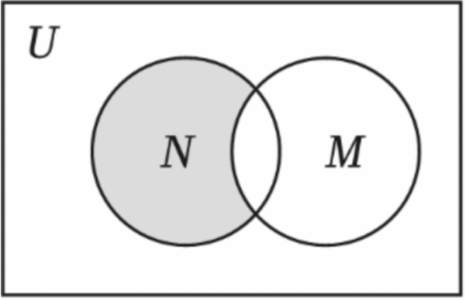
\includegraphics[width=0.30\textwidth]{figures/gao90_q6_venn.png}
\end{center}

\ifanswer
\ans{$N\cap\overline M$}
\fi

\item 已知 $a\in\R$，若关于 $x$ 的方程 $x^2-2x+a-2=0$ 有两个实根 $x_1$、$x_2$，且 $\dfrac1{x_1}+\dfrac1{x_2}=-\dfrac12$，则 $a$ 的值为\blankline[4.4em].

\ifanswer
\solbegin
\step{由于 $x_1$、$x_2$ 是 $x^2-2x+a-2=0$ 的两个实根，}
\step{由韦达定理得 $x_1x_2=a-2$，$x_1+x_2=2$，}
\step{因此 $\dfrac1{x_1}+\dfrac1{x_2}=\dfrac{x_1+x_2}{x_1x_2}=\dfrac2{a-2}=-\dfrac12$，所以 $a-2=-4$，解得 $a=-2$，}
\step{判别式 $\Delta=(-2)^2-4(a-2)=-4a+12$，当 $a=-2$ 时，$\Delta=8+12=20>0$，有两个实根，符合条件，故 $a=-2$.}
\solend
\fi

\item 如果 $-1<x<4$，$-6<y<2$，则 $2x-y$ 的取值范围是\blankline[4.4em].

\ifanswer
\solbegin
\step{因为 $-1<x<4$，$-6<y<2$，所以 $-2<2x<8$，$-2<-y<6$，}
\step{则 $-2+(-2)<2x-y<8+6$，即 $-4<2x-y<14$，}
\step{故 $2x-y$ 的取值范围为 $(-4,14)$.}
\solend
\fi

\item 集合 $A=\left\{x\left|\dfrac6{3-x}\in\Z,x\in\N\right.\right\}$，试用列举法表示集合 $A=\blankline[4.4em]$.

\ifanswer
\solbegin
\step{集合 $A=\left\{x\left|\dfrac6{3-x}\in\Z,x\in\N\right.\right\}$，所以 $3-x$ 可取的值有 $\pm1$、$\pm2$、$\pm3$、$\pm6$，}
\step{又因为 $x\in\N$，所以 $x\in\{0,1,2,4,5,6,9\}$，即 $A=\{0,1,2,4,5,6,9\}$.}
\solend
\fi

\item 不等式 $x^2-ax-b<0$ 的解集是 $(2,3)$，若关于 $x$ 的不等式组 $\begin{cases}(x-a)(3x+b)<0\\ x>t\end{cases}$ 没有实数解，则实数 $t$ 的取值范围是\blankline[4.4em].

\ifanswer
\solbegin
\step{因为等式 $x^2-ax-b<0$ 的解集是 $(2,3)$，所以 $x^2-ax-b=0$ 的根为 $2$、$3$，}
\step{所以 $2+3=a$，$2\times3=-b$，所以 $a=5$，$b=-6$，}
\step{由 $(x-a)(3x+b)=(x-5)(3x-6)<0$ 得 $2<x<5$，}
\step{若关于 $x$ 的不等式组 $\begin{cases}(x-a)(3x+b)<0\\ x>t\end{cases}$ 没有实数解，则 $t\geqslant5$.}
\solend
\fi

\item 若方程 $x^2+2x-m=0$ 有解，则 $m\geqslant a$ 为真命题，则 $a$ 的取值范围为\blankline[4.4em].

\ifanswer
\solbegin
\step{因为方程 $x^2+2x-m=0$ 有解，}
\step{所以 $\Delta=2^2-4\times1\times(-m)=4+4m\geqslant0$，解得 $m\geqslant-1$，}
\step{命题“若方程有解，则 $m\geqslant a$”为真命题，即 $\forall m\in[-1,+\infty)$，$m\geqslant a$ 恒成立，}
\step{因此 $a$ 的取值不能超过集合 $[-1,+\infty)$ 的最小值，即 $a\leqslant-1$，}
\step{综上，$a$ 的取值范围为 $(-\infty,-1]$.}
\solend
\fi

\item 设数集 $M=\left\{x\left|m\leqslant x\leqslant m+\dfrac45\right.\right\}$，$N=\left\{x\left|n-\dfrac14\leqslant x\leqslant n\right.\right\}$，且集合 $M$、$N$ 都是集合 $U=\{x\mid0\leqslant x\leqslant1\}$ 的子集，如果把 $b-a$ 称为非空集合 $\{x\mid a\leqslant x\leqslant b\}$ 的“长度”，那么集合 $M\cap N$ 的“长度”的取值范围为\blankline[4.4em].

\ifanswer
\solbegin
\step{注意到集合 $M$ 的长度为 $\dfrac45$，集合 $N$ 的长度为 $\dfrac14$，均为定值，}
\step{要使得 $M\cap N$ 的“长度”最小，则 $M$ 和 $N$ 尽可能分散到区间的两边，}
\step{长度最小为 $\dfrac45+\dfrac14-1=\dfrac1{20}$；}
\step{要使得 $M\cap N$ 的“长度”最大，则 $M$ 和 $N$ 尽可能集中，}
\step{长度最大就是集合 $N$ 的长度，为 $\dfrac14$，}
\step{故集合 $M\cap N$ 的“长度”的取值范围为 $\left[\dfrac1{20},\dfrac14\right]$.}
\solend
\fi

\end{enumerate}

\bigsec{二、选择题}

\begin{enumerate}
\setcounter{enumi}{12}

\item 设集合 $A=\{x\mid x=2k+1,k\in\Z\}$，$B=\{x\mid x=2k-1,k\in\Z\}$，则 $A$、$B$ 之间的关系是\mbox{（\quad）}

\keepwithprev
A. $B\subsetneq A$\qquad B. $A\subsetneq B$\qquad C. $A=B$\qquad D. 以上都不是

\ifanswer
\solbegin
\step{因为 $k\in\Z$，所以 $2k+1$ 与 $2k-1$ 均表示全体奇数，}
\step{即集合 $A=\{x\mid x=2k+1,k\in\Z\}$ 与 $B=\{x\mid x=2k-1,k\in\Z\}$}
\step{都表示全体奇数构成的集合，所以 $A=B$. 故选 $C$.}
\solend
\fi

\item 已知 $a$、$b\in\R$，且 $a>b$，则下列不等式中一定成立的是\mbox{（\quad）}

\keepwithprev
A. $a+1>b$\qquad B. $a>b+1$\qquad C. $a+1<b+1$\qquad D. $a-1<b-1$

\ifanswer
\solbegin
\step{因为 $a>b$，所以 $a+1>b+1$，$a-1>b-1$，故 $CD$ 错误；}
\step{因为 $a>b$，所以 $a+1>b+0$，即 $a+1>b$ 恒成立，故 $A$ 正确；}
\step{取 $a=1$，$b=0$，$B$ 显然错误.}
\step{故选 $A$.}
\solend
\fi

\item 设 $a$、$b\in\R$，“$a+b>2$ 且 $ab>1$”是“$a>1$，$b>1$”的\mbox{（\quad）}

\keepwithprev
A. 充分不必要条件\qquad B. 必要不充分条件

C. 充要条件\qquad D. 既不充分又不必要条件

\ifanswer
\solbegin
\step{因为 $a>1$ 且 $b>1$，所以 $a+b>2$ 且 $ab>1$，}
\step{若已知 $a+b>2$ 且 $ab>1$，可取 $a=\dfrac12$，$b=8$，也满足已知，}
\step{所以“$a+b>2$ 且 $ab>1$”是“$a>1$ 且 $b>1$”的必要不充分条件，故选 $B$.}
\solend
\fi

\item 设集合 $P_1=\{x\mid x^2+ax+1>0\}$，$P_2=\{x\mid x^2+ax+2>0\}$，$Q_1=\{x\mid x^2+x+b>0\}$，$Q_2=\{x\mid x^2+2x+b>0\}$，其中 $a$、$b\in\R$，下列说法中正确的是\mbox{（\quad）}

\keepwithprev
A. 对任意 $a$，$P_1$ 是 $P_2$ 的子集，对任意 $b$，$Q_1$ 不是 $Q_2$ 的子集

B. 对任意 $a$，$P_1$ 是 $P_2$ 的子集，存在 $b$，使得 $Q_1$ 是 $Q_2$ 的子集

C. 存在 $a$，使得 $P_1$ 不是 $P_2$ 的子集，对任意 $b$，$Q_1$ 不是 $Q_2$ 的子集

D. 存在 $a$，使得 $P_1$ 不是 $P_2$ 的子集，存在 $b$，使得 $Q_1$ 是 $Q_2$ 的子集

\ifanswer
\solbegin
\step{对于集合 $P_1=\{x\mid x^2+ax+1>0\}$，$P_2=\{x\mid x^2+ax+2>0\}$，}
\step{得当 $m\in P_1$ 时，即 $m^2+am+1>0$，得 $m^2+am+2>0$，}
\step{即有 $m\in P_2$，得对任意 $a$，$P_1$ 是 $P_2$ 的子集，}
\step{对于集合 $Q_1=\{x\mid x^2+x+b>0\}$，$Q_2=\{x\mid x^2+2x+b>0\}$，}
\step{当 $b=6$ 时，$Q_1=\{x\mid x^2+x+6>0\}=\R$，$Q_2=\{x\mid x^2+2x+6>0\}=\R$，}
\step{得 $Q_1$ 是 $Q_2$ 的子集，}
\step{当 $b=1$ 时，$Q_1=\{x\mid x^2+x+1>0\}=\R$，}
\step{$Q_2=\{x\mid x^2+2x+1>0\}=\{x\mid x\neq-1\}$，得 $Q_1$ 不是 $Q_2$ 的子集，}
\step{所以存在 $b$，使得 $Q_1$ 是 $Q_2$ 的子集，故选 $B$.}
\solend
\fi

\end{enumerate}

\bigsec{三、解答题}

\begin{enumerate}
\setcounter{enumi}{16}

\item 若 $a$、$b\in\R$，求关于 $x$ 的不等式 $ax\geqslant b$ 的解集.

\ansspace*[9]

\ifanswer
\solbegin
\step{当 $a>0$ 时，原不等式的解集为 $\left\{x\left|x\geqslant\dfrac ba\right.\right\}$；}
\step{当 $a<0$ 时，原不等式的解集为 $\left\{x\left|x\leqslant\dfrac ba\right.\right\}$；}
\step{当 $a=0$，$b\leqslant0$ 时，原不等式的解集为 $\R$；}
\step{当 $a=0$，$b>0$ 时，原不等式的解集为 $\varnothing$.}
\solend
\fi

\item 设集合 $A=\{x\mid x^2+3x+2=0\}$，$B=\{x\mid x^2+(m+1)x+m=0\}$.

（1）用列举法表示集合 $A$；

（2）若 $B\subseteq A$，求实数 $m$ 的值.

\ansspace*[9]

\ifanswer
\solbegin
\stepm{（1）}{集合 $A=\{x\mid x^2+3x+2=0\}$，解方程 $x^2+3x+2=0$，得 $x_1=-2$，$x_2=-1$，}
\step{所以 $A=\{-2,-1\}$.}
\stepm{（2）}{$A=\{-2,-1\}$，$B=\{x\mid x^2+(m+1)x+m=0\}=\{x\mid(x+1)(x+m)=0\}$，}
\step{$B\subseteq A$，所以 $m=1$ 或 $m=2$，所以实数 $m$ 的值为 $1$ 或 $2$.}
\solend
\fi

\item （1）设 $a$、$b$ 是两个正数. 已知 $a>b$，比较 $\dfrac{2a+b}{a+2b}$ 与 $\dfrac ab$ 的值的大小.

（2）用反证法证明：若 $a$、$b\in\R$，且 $x=a^2-2b+1$，$y=b^2-2a+1$，则 $x$、$y$ 中至少有一个不小于 $0$.

\ansspace*[12]

\ifanswer
\solbegin
\stepm{（1）}{$\dfrac{2a+b}{a+2b}-\dfrac ab=\dfrac{b(2a+b)}{b(a+2b)}-\dfrac{a(a+2b)}{b(a+2b)}=\dfrac{b(2a+b)-a(a+2b)}{b(a+2b)}$}
\step{$=\dfrac{2ab+b^2-a^2-2ab}{b(a+2b)}=\dfrac{b^2-a^2}{b(a+2b)}=\dfrac{(b+a)(b-a)}{b(a+2b)}$，}
\step{又 $a>0$，$b>0$，$a>b$，所以 $b+a>0$，$b-a<0$，$b(a+2b)>0$，}
\step{所以 $\dfrac{(b+a)(b-a)}{b(a+2b)}<0$，即 $\dfrac{2a+b}{a+2b}-\dfrac ab<0$，所以 $\dfrac{2a+b}{a+2b}<\dfrac ab$.}
\stepm{（2）}{假设 $x$、$y$ 都小于 $0$，则有 $x+y<0$，}
\step{因为 $x=a^2-2b+1$，$y=b^2-2a+1$，}
\step{所以 $x+y=(a^2-2b+1)+(b^2-2a+1)=(a^2-2a+1)+(b^2-2b+1)$}
\step{$=(a-1)^2+(b-1)^2$，}
\step{又 $a$、$b\in\R$，所以 $(a-1)^2\geqslant0$，$(b-1)^2\geqslant0$，即 $x+y\geqslant0$，}
\step{这与 $x+y<0$ 矛盾，故假设不成立，所以 $x$、$y$ 中至少有一个不小于 $0$.}
\solend
\fi

\item 已知 $m>0$，$p:(x+1)(x-5)\leqslant0$，$q:1-m\leqslant x\leqslant1+m$.

（1）若 $m=5$，$p$、$q$ 有且只有一个为真命题，求实数 $x$ 的取值范围；

（2）若 $p$ 是 $q$ 的充分不必要条件，求实数 $m$ 的取值范围.

\ansspace*[12]

\ifanswer
\solbegin
\stepm{（1）}{对于 $p:(x+1)(x-5)\leqslant0$，解得 $-1\leqslant x\leqslant5$，}
\step{若 $m=5$，则 $q:-4\leqslant x\leqslant6$，}
\step{若 $m=5$，$p$、$q$ 有且只有一个为真命题，则 $p$ 真 $q$ 假或 $p$ 假 $q$ 真，}
\step{若 $p$ 真 $q$ 假，即 $\begin{cases}-1\leqslant x\leqslant5\\ x<-4\ \text{或}\ x>6\end{cases}$，无解，}
\step{若 $p$ 假 $q$ 真，即 $\begin{cases}x<-1\ \text{或}\ x>5\\ -4\leqslant x\leqslant6\end{cases}$，解得 $-4\leqslant x<-1$ 或 $5<x\leqslant6$，}
\step{综上，$-4\leqslant x<-1$ 或 $5<x\leqslant6$，即 $x$ 的取值范围为 $[-4,-1)\cup(5,6]$；}
\stepm{（2）}{若 $p$ 是 $q$ 的充分条件，则有 $\begin{cases}1-m\leqslant-1\\ 5\leqslant1+m\end{cases}$，解得 $m\geqslant4$，}
\step{即 $m$ 的取值范围为 $[4,+\infty)$.}
\solend
\fi

\item 已知关于 $x$ 的不等式：$ax^2-(a+1)x+1<0(a\in\R)$.

（1）当 $a=-2$ 时，求不等式的解集；

（2）当 $a\geqslant0$ 时，求不等式的解集；

（3）命题 $P$：若二次不等式 $ax^2-(a+1)x+1<0$ 的解集为空集，命题 $Q:x^2-2x-a^2+a+1>0$ 对任意实数 $x$ 都成立，若 $P$、$Q$ 中至少有一个真命题，求实数 $a$ 的取值范围.

\ansspace*[14]

\ifanswer
\solbegin
\stepm{（1）}{当 $a=-2$ 时，原不等式为 $2x^2-x-1>0$，即 $(x-1)(2x+1)>0$，}
\step{解得 $x<-\dfrac12$ 或 $x>1$，所以原不等式的解集为 $\left(-\infty,-\dfrac12\right)\cup(1,+\infty)$.}
\stepm{（2）}{当 $a=0$ 时，原不等式为 $-x+1<0$，解得 $x>1$；}
\step{当 $a>0$ 时，原不等式变为 $(ax-1)(x-1)<0$，其对应方程的两根为 $\dfrac1a$，$1$，}
\step{若 $\dfrac1a<1$，即 $a>1$ 时，由 $(ax-1)(x-1)<0$ 解得 $\dfrac1a<x<1$，}
\step{若 $\dfrac1a=1$，即 $a=1$ 时，不等式 $(ax-1)(x-1)<0$ 解集为 $\varnothing$，}
\step{若 $\dfrac1a>1$，即 $0<a<1$ 时，由 $(ax-1)(x-1)<0$ 解得 $1<x<\dfrac1a$，}
\step{综上，当 $a=0$ 时，不等式的解集为 $(1,+\infty)$，}
\step{当 $0<a<1$ 时，不等式的解集为 $\left(1,\dfrac1a\right)$，}
\step{当 $a=1$ 时，不等式的解集为 $\varnothing$，}
\step{当 $a>1$ 时，不等式的解集为 $\left(\dfrac1a,1\right)$.}
\stepm{（3）}{若命题 $P$ 为真命题，}
\step{若 $a<0$，原不等式变为 $(ax-1)(x-1)<0$，其对应方程的两根为 $\dfrac1a$，$1$，}
\step{其解集为 $\left(-\infty,\dfrac1a\right)\cup(1,+\infty)$，不合题意，}
\step{当 $a\geqslant0$ 时，由（2）得当 $a=1$ 时，解集为 $\varnothing$，}
\step{所以命题 $P$ 为真命题，则 $a=1$；}
\step{命题 $Q$ 为真命题，则有相应方程的 $\Delta<0$，即 $a^2-a<0$，解得 $0<a<1$；}
\step{所以当命题 $P$、$Q$ 都为假命题时，$\begin{cases}a\leqslant0\ \text{或}\ a\geqslant1\\ a\neq1\end{cases}$，解得 $a\leqslant0$ 或 $a>1$，}
\step{所以命题 $P$、$Q$ 中至少有一个真命题，则 $0<a\leqslant1$.}
\step{所以实数 $a$ 的取值范围为 $(0,1]$.}
\solend
\fi

\end{enumerate}

\end{document}
"
% 紧凑版：xelatex "\def\iscompact{1}% 高一90_杨思高级中学_10月月考.tex
%   —— 高一上数学“2026-2027 年杨思高级中学高一上 10 月月考”（讲评版）
% 试卷版：xelatex 高一90_杨思高级中学_10月月考.tex
% 答案版：xelatex "\def\isanswer{1}\input{高一90_杨思高级中学_10月月考.tex}"
% 紧凑版：xelatex "\def\iscompact{1}\input{高一90_杨思高级中学_10月月考.tex}"
%
% 原始材料：微信公众号“魔都数学加油站”文章，连载“27学年高一90”；
% 原文标题“27学年高一90——2026-2027年上海市杨思高级中学高一上10月月考”；
% 原文链接：https://mp.weixin.qq.com/s/pvQC5fkWu5Jj3C7dF3-Exw。
% 正文为 8 张 PNG 页（`原图/高一90_杨思高级中学_10月月考/01..08.png`），
% 尺寸混排（第 1、6 页为 2560×3620，其余为 4762×6735），均按页序读取。
%
% 篇幅与题号：原卷自第 3 题起编号（第 1、2 题不在原文内）。填空题 3—12（10 题）、
% 选择题 13—16（4 题）、解答题 17—21（5 题），共 19 题。
%
% 讲评版：第 6 题只印【答案】（“$N\cap\overline M$”），本稿只给 \ans{}；
% 其余 18 题印【解析】，其中选择题答案在解析末句“故选 C／A／B／B”。
% 第 6 题题干带一幅韦恩图（全集 $U$、集合 $M$、$N$ 与阴影部分），三版都出。
%
% 副标题：原卷未印副标题。本稿按内容标作“集合与常用逻辑用语、不等式”。
%
% 原卷笔误/存疑（均照录未改，正文对应处另有 % 注）：
%   ① 第 6 题的韦恩图阴影为 $N$ 中不属于 $M$ 的部分，与所印答案 $N\cap\overline M$ 一致；
%      图与答案均照录。原卷把“（请用各集合的交，并，补表示）”的逗号排作全角逗号，照录；
%   ② 第 12 题题干“如果把 $b-a$ 称为非空集合 $\{x\mid a\leqslant x\leqslant b\}$ 的‘长度’”
%      与本稿统一后的 $\R$、$\Z$、$\N$ 记号无关，原文用斜体 $R$、$Z$、$N$，按惯例改写。
%
% 与原卷的排版差异：
%   ① 原卷每题下直接印【答案】/【解析】，本稿按全稿惯例将答案与解析置于答案版；
%   ② 原卷未印副标题，本稿补出；填空横线统一排 \blankline[4.4em]；
%   ③ 原卷数集记号排斜体 $R$、$Z$、$N$，本稿按全稿惯例改用 $\R$、$\Z$、$\N$；
%   ④ 第 17—21 题的子问用行内“（1）（2）（3）”段，解析中的子问标号用 \stepm；
%   ⑤ 解答题按惯例加 \ansspace；选择题括号排 \mbox{（\quad）}；
%   ⑥ 第 6 题的韦恩图原卷排在题干右侧、文字绕排，本稿改排为题干后的居中图
%      （自原图裁切、去粉色水印后转灰度）。
%
% 行数核对：逐题数 \step/\stepm 条数，合计 94 条（Q3：2；Q4：2；Q5：1；Q6：0；
% Q7：4；Q8：3；Q9：2；Q10：4；Q11：5；Q12：6；Q13：3；Q14：4；Q15：3；Q16：9；
% Q17：4；Q18：4；Q19：10；Q20：8；Q21：20）。第 6 题只印【答案】，不计入 \step 账。
% 原卷解析的换行按语意合并，未逐行强拆。
%
\documentclass[a4paper,11pt]{article}
\usepackage{common}

\begin{document}

\examtitlest[7]{2026--2027 年杨思高级中学高一上 10 月月考}{集合与常用逻辑用语、不等式}

\bigsec{一、填空题}

\begin{enumerate}
\setcounter{enumi}{2}

\item 已知集合 $A=\{x\mid6x+a>0\}$，若 $1\notin A$，则实数 $a$ 的取值范围是\blankline[4.4em].

\ifanswer
\solbegin
\step{集合 $A=\{x\mid6x+a>0\}$，若 $1\notin A$，则 $6+a\leqslant0$ 恒成立，故 $a\leqslant-6$，}
\step{故实数 $a$ 的取值范围是 $(-\infty,-6]$.}
\solend
\fi

\item 设全集 $U=\R$，集合 $A=\{x\mid-1\leqslant x\leqslant1\}$，$B=\{x\mid0<x<2\}$，则 $\overline{A\cup B}=\blankline[4.4em]$.

\ifanswer
\solbegin
\step{$B=\{x\mid0<x<2\}$，$A=\{x\mid-1\leqslant x\leqslant1\}$，所以 $A\cup B=\{x\mid-1\leqslant x<2\}$，}
\step{又因为全集 $U=\R$，所以 $\overline{A\cup B}=(-\infty,-1)\cup[2,+\infty)$.}
\solend
\fi

\item 集合 $A=\{(x,y)\mid y=-x\}$，$B=\{(x,y)\mid y=2x-4\}$，则 $A\cap B=\blankline[4.4em]$.

\ifanswer
\solbegin
\step{联立 $\begin{cases}y=-x\\ y=2x-4\end{cases}$，解得 $\begin{cases}x=\dfrac43\\[0.2em] y=-\dfrac43\end{cases}$，即 $A\cap B=\left\{\left(\dfrac43,-\dfrac43\right)\right\}$.}
\solend
\fi

\item 设 $U$ 是全集，$M$、$N$ 是 $U$ 的子集，则图中阴影部分所表示的集合是\blankline[4.4em].

（请用各集合的交，并，补表示）

\begin{center}
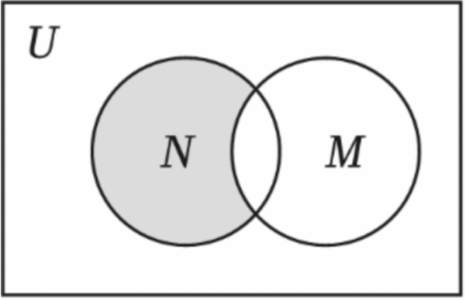
\includegraphics[width=0.30\textwidth]{figures/gao90_q6_venn.png}
\end{center}

\ifanswer
\ans{$N\cap\overline M$}
\fi

\item 已知 $a\in\R$，若关于 $x$ 的方程 $x^2-2x+a-2=0$ 有两个实根 $x_1$、$x_2$，且 $\dfrac1{x_1}+\dfrac1{x_2}=-\dfrac12$，则 $a$ 的值为\blankline[4.4em].

\ifanswer
\solbegin
\step{由于 $x_1$、$x_2$ 是 $x^2-2x+a-2=0$ 的两个实根，}
\step{由韦达定理得 $x_1x_2=a-2$，$x_1+x_2=2$，}
\step{因此 $\dfrac1{x_1}+\dfrac1{x_2}=\dfrac{x_1+x_2}{x_1x_2}=\dfrac2{a-2}=-\dfrac12$，所以 $a-2=-4$，解得 $a=-2$，}
\step{判别式 $\Delta=(-2)^2-4(a-2)=-4a+12$，当 $a=-2$ 时，$\Delta=8+12=20>0$，有两个实根，符合条件，故 $a=-2$.}
\solend
\fi

\item 如果 $-1<x<4$，$-6<y<2$，则 $2x-y$ 的取值范围是\blankline[4.4em].

\ifanswer
\solbegin
\step{因为 $-1<x<4$，$-6<y<2$，所以 $-2<2x<8$，$-2<-y<6$，}
\step{则 $-2+(-2)<2x-y<8+6$，即 $-4<2x-y<14$，}
\step{故 $2x-y$ 的取值范围为 $(-4,14)$.}
\solend
\fi

\item 集合 $A=\left\{x\left|\dfrac6{3-x}\in\Z,x\in\N\right.\right\}$，试用列举法表示集合 $A=\blankline[4.4em]$.

\ifanswer
\solbegin
\step{集合 $A=\left\{x\left|\dfrac6{3-x}\in\Z,x\in\N\right.\right\}$，所以 $3-x$ 可取的值有 $\pm1$、$\pm2$、$\pm3$、$\pm6$，}
\step{又因为 $x\in\N$，所以 $x\in\{0,1,2,4,5,6,9\}$，即 $A=\{0,1,2,4,5,6,9\}$.}
\solend
\fi

\item 不等式 $x^2-ax-b<0$ 的解集是 $(2,3)$，若关于 $x$ 的不等式组 $\begin{cases}(x-a)(3x+b)<0\\ x>t\end{cases}$ 没有实数解，则实数 $t$ 的取值范围是\blankline[4.4em].

\ifanswer
\solbegin
\step{因为等式 $x^2-ax-b<0$ 的解集是 $(2,3)$，所以 $x^2-ax-b=0$ 的根为 $2$、$3$，}
\step{所以 $2+3=a$，$2\times3=-b$，所以 $a=5$，$b=-6$，}
\step{由 $(x-a)(3x+b)=(x-5)(3x-6)<0$ 得 $2<x<5$，}
\step{若关于 $x$ 的不等式组 $\begin{cases}(x-a)(3x+b)<0\\ x>t\end{cases}$ 没有实数解，则 $t\geqslant5$.}
\solend
\fi

\item 若方程 $x^2+2x-m=0$ 有解，则 $m\geqslant a$ 为真命题，则 $a$ 的取值范围为\blankline[4.4em].

\ifanswer
\solbegin
\step{因为方程 $x^2+2x-m=0$ 有解，}
\step{所以 $\Delta=2^2-4\times1\times(-m)=4+4m\geqslant0$，解得 $m\geqslant-1$，}
\step{命题“若方程有解，则 $m\geqslant a$”为真命题，即 $\forall m\in[-1,+\infty)$，$m\geqslant a$ 恒成立，}
\step{因此 $a$ 的取值不能超过集合 $[-1,+\infty)$ 的最小值，即 $a\leqslant-1$，}
\step{综上，$a$ 的取值范围为 $(-\infty,-1]$.}
\solend
\fi

\item 设数集 $M=\left\{x\left|m\leqslant x\leqslant m+\dfrac45\right.\right\}$，$N=\left\{x\left|n-\dfrac14\leqslant x\leqslant n\right.\right\}$，且集合 $M$、$N$ 都是集合 $U=\{x\mid0\leqslant x\leqslant1\}$ 的子集，如果把 $b-a$ 称为非空集合 $\{x\mid a\leqslant x\leqslant b\}$ 的“长度”，那么集合 $M\cap N$ 的“长度”的取值范围为\blankline[4.4em].

\ifanswer
\solbegin
\step{注意到集合 $M$ 的长度为 $\dfrac45$，集合 $N$ 的长度为 $\dfrac14$，均为定值，}
\step{要使得 $M\cap N$ 的“长度”最小，则 $M$ 和 $N$ 尽可能分散到区间的两边，}
\step{长度最小为 $\dfrac45+\dfrac14-1=\dfrac1{20}$；}
\step{要使得 $M\cap N$ 的“长度”最大，则 $M$ 和 $N$ 尽可能集中，}
\step{长度最大就是集合 $N$ 的长度，为 $\dfrac14$，}
\step{故集合 $M\cap N$ 的“长度”的取值范围为 $\left[\dfrac1{20},\dfrac14\right]$.}
\solend
\fi

\end{enumerate}

\bigsec{二、选择题}

\begin{enumerate}
\setcounter{enumi}{12}

\item 设集合 $A=\{x\mid x=2k+1,k\in\Z\}$，$B=\{x\mid x=2k-1,k\in\Z\}$，则 $A$、$B$ 之间的关系是\mbox{（\quad）}

\keepwithprev
A. $B\subsetneq A$\qquad B. $A\subsetneq B$\qquad C. $A=B$\qquad D. 以上都不是

\ifanswer
\solbegin
\step{因为 $k\in\Z$，所以 $2k+1$ 与 $2k-1$ 均表示全体奇数，}
\step{即集合 $A=\{x\mid x=2k+1,k\in\Z\}$ 与 $B=\{x\mid x=2k-1,k\in\Z\}$}
\step{都表示全体奇数构成的集合，所以 $A=B$. 故选 $C$.}
\solend
\fi

\item 已知 $a$、$b\in\R$，且 $a>b$，则下列不等式中一定成立的是\mbox{（\quad）}

\keepwithprev
A. $a+1>b$\qquad B. $a>b+1$\qquad C. $a+1<b+1$\qquad D. $a-1<b-1$

\ifanswer
\solbegin
\step{因为 $a>b$，所以 $a+1>b+1$，$a-1>b-1$，故 $CD$ 错误；}
\step{因为 $a>b$，所以 $a+1>b+0$，即 $a+1>b$ 恒成立，故 $A$ 正确；}
\step{取 $a=1$，$b=0$，$B$ 显然错误.}
\step{故选 $A$.}
\solend
\fi

\item 设 $a$、$b\in\R$，“$a+b>2$ 且 $ab>1$”是“$a>1$，$b>1$”的\mbox{（\quad）}

\keepwithprev
A. 充分不必要条件\qquad B. 必要不充分条件

C. 充要条件\qquad D. 既不充分又不必要条件

\ifanswer
\solbegin
\step{因为 $a>1$ 且 $b>1$，所以 $a+b>2$ 且 $ab>1$，}
\step{若已知 $a+b>2$ 且 $ab>1$，可取 $a=\dfrac12$，$b=8$，也满足已知，}
\step{所以“$a+b>2$ 且 $ab>1$”是“$a>1$ 且 $b>1$”的必要不充分条件，故选 $B$.}
\solend
\fi

\item 设集合 $P_1=\{x\mid x^2+ax+1>0\}$，$P_2=\{x\mid x^2+ax+2>0\}$，$Q_1=\{x\mid x^2+x+b>0\}$，$Q_2=\{x\mid x^2+2x+b>0\}$，其中 $a$、$b\in\R$，下列说法中正确的是\mbox{（\quad）}

\keepwithprev
A. 对任意 $a$，$P_1$ 是 $P_2$ 的子集，对任意 $b$，$Q_1$ 不是 $Q_2$ 的子集

B. 对任意 $a$，$P_1$ 是 $P_2$ 的子集，存在 $b$，使得 $Q_1$ 是 $Q_2$ 的子集

C. 存在 $a$，使得 $P_1$ 不是 $P_2$ 的子集，对任意 $b$，$Q_1$ 不是 $Q_2$ 的子集

D. 存在 $a$，使得 $P_1$ 不是 $P_2$ 的子集，存在 $b$，使得 $Q_1$ 是 $Q_2$ 的子集

\ifanswer
\solbegin
\step{对于集合 $P_1=\{x\mid x^2+ax+1>0\}$，$P_2=\{x\mid x^2+ax+2>0\}$，}
\step{得当 $m\in P_1$ 时，即 $m^2+am+1>0$，得 $m^2+am+2>0$，}
\step{即有 $m\in P_2$，得对任意 $a$，$P_1$ 是 $P_2$ 的子集，}
\step{对于集合 $Q_1=\{x\mid x^2+x+b>0\}$，$Q_2=\{x\mid x^2+2x+b>0\}$，}
\step{当 $b=6$ 时，$Q_1=\{x\mid x^2+x+6>0\}=\R$，$Q_2=\{x\mid x^2+2x+6>0\}=\R$，}
\step{得 $Q_1$ 是 $Q_2$ 的子集，}
\step{当 $b=1$ 时，$Q_1=\{x\mid x^2+x+1>0\}=\R$，}
\step{$Q_2=\{x\mid x^2+2x+1>0\}=\{x\mid x\neq-1\}$，得 $Q_1$ 不是 $Q_2$ 的子集，}
\step{所以存在 $b$，使得 $Q_1$ 是 $Q_2$ 的子集，故选 $B$.}
\solend
\fi

\end{enumerate}

\bigsec{三、解答题}

\begin{enumerate}
\setcounter{enumi}{16}

\item 若 $a$、$b\in\R$，求关于 $x$ 的不等式 $ax\geqslant b$ 的解集.

\ansspace*[9]

\ifanswer
\solbegin
\step{当 $a>0$ 时，原不等式的解集为 $\left\{x\left|x\geqslant\dfrac ba\right.\right\}$；}
\step{当 $a<0$ 时，原不等式的解集为 $\left\{x\left|x\leqslant\dfrac ba\right.\right\}$；}
\step{当 $a=0$，$b\leqslant0$ 时，原不等式的解集为 $\R$；}
\step{当 $a=0$，$b>0$ 时，原不等式的解集为 $\varnothing$.}
\solend
\fi

\item 设集合 $A=\{x\mid x^2+3x+2=0\}$，$B=\{x\mid x^2+(m+1)x+m=0\}$.

（1）用列举法表示集合 $A$；

（2）若 $B\subseteq A$，求实数 $m$ 的值.

\ansspace*[9]

\ifanswer
\solbegin
\stepm{（1）}{集合 $A=\{x\mid x^2+3x+2=0\}$，解方程 $x^2+3x+2=0$，得 $x_1=-2$，$x_2=-1$，}
\step{所以 $A=\{-2,-1\}$.}
\stepm{（2）}{$A=\{-2,-1\}$，$B=\{x\mid x^2+(m+1)x+m=0\}=\{x\mid(x+1)(x+m)=0\}$，}
\step{$B\subseteq A$，所以 $m=1$ 或 $m=2$，所以实数 $m$ 的值为 $1$ 或 $2$.}
\solend
\fi

\item （1）设 $a$、$b$ 是两个正数. 已知 $a>b$，比较 $\dfrac{2a+b}{a+2b}$ 与 $\dfrac ab$ 的值的大小.

（2）用反证法证明：若 $a$、$b\in\R$，且 $x=a^2-2b+1$，$y=b^2-2a+1$，则 $x$、$y$ 中至少有一个不小于 $0$.

\ansspace*[12]

\ifanswer
\solbegin
\stepm{（1）}{$\dfrac{2a+b}{a+2b}-\dfrac ab=\dfrac{b(2a+b)}{b(a+2b)}-\dfrac{a(a+2b)}{b(a+2b)}=\dfrac{b(2a+b)-a(a+2b)}{b(a+2b)}$}
\step{$=\dfrac{2ab+b^2-a^2-2ab}{b(a+2b)}=\dfrac{b^2-a^2}{b(a+2b)}=\dfrac{(b+a)(b-a)}{b(a+2b)}$，}
\step{又 $a>0$，$b>0$，$a>b$，所以 $b+a>0$，$b-a<0$，$b(a+2b)>0$，}
\step{所以 $\dfrac{(b+a)(b-a)}{b(a+2b)}<0$，即 $\dfrac{2a+b}{a+2b}-\dfrac ab<0$，所以 $\dfrac{2a+b}{a+2b}<\dfrac ab$.}
\stepm{（2）}{假设 $x$、$y$ 都小于 $0$，则有 $x+y<0$，}
\step{因为 $x=a^2-2b+1$，$y=b^2-2a+1$，}
\step{所以 $x+y=(a^2-2b+1)+(b^2-2a+1)=(a^2-2a+1)+(b^2-2b+1)$}
\step{$=(a-1)^2+(b-1)^2$，}
\step{又 $a$、$b\in\R$，所以 $(a-1)^2\geqslant0$，$(b-1)^2\geqslant0$，即 $x+y\geqslant0$，}
\step{这与 $x+y<0$ 矛盾，故假设不成立，所以 $x$、$y$ 中至少有一个不小于 $0$.}
\solend
\fi

\item 已知 $m>0$，$p:(x+1)(x-5)\leqslant0$，$q:1-m\leqslant x\leqslant1+m$.

（1）若 $m=5$，$p$、$q$ 有且只有一个为真命题，求实数 $x$ 的取值范围；

（2）若 $p$ 是 $q$ 的充分不必要条件，求实数 $m$ 的取值范围.

\ansspace*[12]

\ifanswer
\solbegin
\stepm{（1）}{对于 $p:(x+1)(x-5)\leqslant0$，解得 $-1\leqslant x\leqslant5$，}
\step{若 $m=5$，则 $q:-4\leqslant x\leqslant6$，}
\step{若 $m=5$，$p$、$q$ 有且只有一个为真命题，则 $p$ 真 $q$ 假或 $p$ 假 $q$ 真，}
\step{若 $p$ 真 $q$ 假，即 $\begin{cases}-1\leqslant x\leqslant5\\ x<-4\ \text{或}\ x>6\end{cases}$，无解，}
\step{若 $p$ 假 $q$ 真，即 $\begin{cases}x<-1\ \text{或}\ x>5\\ -4\leqslant x\leqslant6\end{cases}$，解得 $-4\leqslant x<-1$ 或 $5<x\leqslant6$，}
\step{综上，$-4\leqslant x<-1$ 或 $5<x\leqslant6$，即 $x$ 的取值范围为 $[-4,-1)\cup(5,6]$；}
\stepm{（2）}{若 $p$ 是 $q$ 的充分条件，则有 $\begin{cases}1-m\leqslant-1\\ 5\leqslant1+m\end{cases}$，解得 $m\geqslant4$，}
\step{即 $m$ 的取值范围为 $[4,+\infty)$.}
\solend
\fi

\item 已知关于 $x$ 的不等式：$ax^2-(a+1)x+1<0(a\in\R)$.

（1）当 $a=-2$ 时，求不等式的解集；

（2）当 $a\geqslant0$ 时，求不等式的解集；

（3）命题 $P$：若二次不等式 $ax^2-(a+1)x+1<0$ 的解集为空集，命题 $Q:x^2-2x-a^2+a+1>0$ 对任意实数 $x$ 都成立，若 $P$、$Q$ 中至少有一个真命题，求实数 $a$ 的取值范围.

\ansspace*[14]

\ifanswer
\solbegin
\stepm{（1）}{当 $a=-2$ 时，原不等式为 $2x^2-x-1>0$，即 $(x-1)(2x+1)>0$，}
\step{解得 $x<-\dfrac12$ 或 $x>1$，所以原不等式的解集为 $\left(-\infty,-\dfrac12\right)\cup(1,+\infty)$.}
\stepm{（2）}{当 $a=0$ 时，原不等式为 $-x+1<0$，解得 $x>1$；}
\step{当 $a>0$ 时，原不等式变为 $(ax-1)(x-1)<0$，其对应方程的两根为 $\dfrac1a$，$1$，}
\step{若 $\dfrac1a<1$，即 $a>1$ 时，由 $(ax-1)(x-1)<0$ 解得 $\dfrac1a<x<1$，}
\step{若 $\dfrac1a=1$，即 $a=1$ 时，不等式 $(ax-1)(x-1)<0$ 解集为 $\varnothing$，}
\step{若 $\dfrac1a>1$，即 $0<a<1$ 时，由 $(ax-1)(x-1)<0$ 解得 $1<x<\dfrac1a$，}
\step{综上，当 $a=0$ 时，不等式的解集为 $(1,+\infty)$，}
\step{当 $0<a<1$ 时，不等式的解集为 $\left(1,\dfrac1a\right)$，}
\step{当 $a=1$ 时，不等式的解集为 $\varnothing$，}
\step{当 $a>1$ 时，不等式的解集为 $\left(\dfrac1a,1\right)$.}
\stepm{（3）}{若命题 $P$ 为真命题，}
\step{若 $a<0$，原不等式变为 $(ax-1)(x-1)<0$，其对应方程的两根为 $\dfrac1a$，$1$，}
\step{其解集为 $\left(-\infty,\dfrac1a\right)\cup(1,+\infty)$，不合题意，}
\step{当 $a\geqslant0$ 时，由（2）得当 $a=1$ 时，解集为 $\varnothing$，}
\step{所以命题 $P$ 为真命题，则 $a=1$；}
\step{命题 $Q$ 为真命题，则有相应方程的 $\Delta<0$，即 $a^2-a<0$，解得 $0<a<1$；}
\step{所以当命题 $P$、$Q$ 都为假命题时，$\begin{cases}a\leqslant0\ \text{或}\ a\geqslant1\\ a\neq1\end{cases}$，解得 $a\leqslant0$ 或 $a>1$，}
\step{所以命题 $P$、$Q$ 中至少有一个真命题，则 $0<a\leqslant1$.}
\step{所以实数 $a$ 的取值范围为 $(0,1]$.}
\solend
\fi

\end{enumerate}

\end{document}
"
%
% 原始材料：微信公众号“魔都数学加油站”文章，连载“27学年高一90”；
% 原文标题“27学年高一90——2026-2027年上海市杨思高级中学高一上10月月考”；
% 原文链接：https://mp.weixin.qq.com/s/pvQC5fkWu5Jj3C7dF3-Exw。
% 正文为 8 张 PNG 页（`原图/高一90_杨思高级中学_10月月考/01..08.png`），
% 尺寸混排（第 1、6 页为 2560×3620，其余为 4762×6735），均按页序读取。
%
% 篇幅与题号：原卷自第 3 题起编号（第 1、2 题不在原文内）。填空题 3—12（10 题）、
% 选择题 13—16（4 题）、解答题 17—21（5 题），共 19 题。
%
% 讲评版：第 6 题只印【答案】（“$N\cap\overline M$”），本稿只给 \ans{}；
% 其余 18 题印【解析】，其中选择题答案在解析末句“故选 C／A／B／B”。
% 第 6 题题干带一幅韦恩图（全集 $U$、集合 $M$、$N$ 与阴影部分），三版都出。
%
% 副标题：原卷未印副标题。本稿按内容标作“集合与常用逻辑用语、不等式”。
%
% 原卷笔误/存疑（均照录未改，正文对应处另有 % 注）：
%   ① 第 6 题的韦恩图阴影为 $N$ 中不属于 $M$ 的部分，与所印答案 $N\cap\overline M$ 一致；
%      图与答案均照录。原卷把“（请用各集合的交，并，补表示）”的逗号排作全角逗号，照录；
%   ② 第 12 题题干“如果把 $b-a$ 称为非空集合 $\{x\mid a\leqslant x\leqslant b\}$ 的‘长度’”
%      与本稿统一后的 $\R$、$\Z$、$\N$ 记号无关，原文用斜体 $R$、$Z$、$N$，按惯例改写。
%
% 与原卷的排版差异：
%   ① 原卷每题下直接印【答案】/【解析】，本稿按全稿惯例将答案与解析置于答案版；
%   ② 原卷未印副标题，本稿补出；填空横线统一排 \blankline[4.4em]；
%   ③ 原卷数集记号排斜体 $R$、$Z$、$N$，本稿按全稿惯例改用 $\R$、$\Z$、$\N$；
%   ④ 第 17—21 题的子问用行内“（1）（2）（3）”段，解析中的子问标号用 \stepm；
%   ⑤ 解答题按惯例加 \ansspace；选择题括号排 \mbox{（\quad）}；
%   ⑥ 第 6 题的韦恩图原卷排在题干右侧、文字绕排，本稿改排为题干后的居中图
%      （自原图裁切、去粉色水印后转灰度）。
%
% 行数核对：逐题数 \step/\stepm 条数，合计 94 条（Q3：2；Q4：2；Q5：1；Q6：0；
% Q7：4；Q8：3；Q9：2；Q10：4；Q11：5；Q12：6；Q13：3；Q14：4；Q15：3；Q16：9；
% Q17：4；Q18：4；Q19：10；Q20：8；Q21：20）。第 6 题只印【答案】，不计入 \step 账。
% 原卷解析的换行按语意合并，未逐行强拆。
%
\documentclass[a4paper,11pt]{article}
\usepackage{common}

\begin{document}

\examtitlest[7]{2026--2027 年杨思高级中学高一上 10 月月考}{集合与常用逻辑用语、不等式}

\bigsec{一、填空题}

\begin{enumerate}
\setcounter{enumi}{2}

\item 已知集合 $A=\{x\mid6x+a>0\}$，若 $1\notin A$，则实数 $a$ 的取值范围是\blankline[4.4em].

\ifanswer
\solbegin
\step{集合 $A=\{x\mid6x+a>0\}$，若 $1\notin A$，则 $6+a\leqslant0$ 恒成立，故 $a\leqslant-6$，}
\step{故实数 $a$ 的取值范围是 $(-\infty,-6]$.}
\solend
\fi

\item 设全集 $U=\R$，集合 $A=\{x\mid-1\leqslant x\leqslant1\}$，$B=\{x\mid0<x<2\}$，则 $\overline{A\cup B}=\blankline[4.4em]$.

\ifanswer
\solbegin
\step{$B=\{x\mid0<x<2\}$，$A=\{x\mid-1\leqslant x\leqslant1\}$，所以 $A\cup B=\{x\mid-1\leqslant x<2\}$，}
\step{又因为全集 $U=\R$，所以 $\overline{A\cup B}=(-\infty,-1)\cup[2,+\infty)$.}
\solend
\fi

\item 集合 $A=\{(x,y)\mid y=-x\}$，$B=\{(x,y)\mid y=2x-4\}$，则 $A\cap B=\blankline[4.4em]$.

\ifanswer
\solbegin
\step{联立 $\begin{cases}y=-x\\ y=2x-4\end{cases}$，解得 $\begin{cases}x=\dfrac43\\[0.2em] y=-\dfrac43\end{cases}$，即 $A\cap B=\left\{\left(\dfrac43,-\dfrac43\right)\right\}$.}
\solend
\fi

\item 设 $U$ 是全集，$M$、$N$ 是 $U$ 的子集，则图中阴影部分所表示的集合是\blankline[4.4em].

（请用各集合的交，并，补表示）

\begin{center}
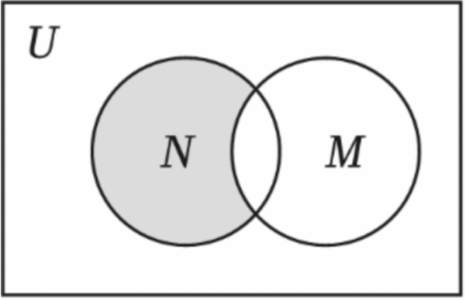
\includegraphics[width=0.30\textwidth]{figures/gao90_q6_venn.png}
\end{center}

\ifanswer
\ans{$N\cap\overline M$}
\fi

\item 已知 $a\in\R$，若关于 $x$ 的方程 $x^2-2x+a-2=0$ 有两个实根 $x_1$、$x_2$，且 $\dfrac1{x_1}+\dfrac1{x_2}=-\dfrac12$，则 $a$ 的值为\blankline[4.4em].

\ifanswer
\solbegin
\step{由于 $x_1$、$x_2$ 是 $x^2-2x+a-2=0$ 的两个实根，}
\step{由韦达定理得 $x_1x_2=a-2$，$x_1+x_2=2$，}
\step{因此 $\dfrac1{x_1}+\dfrac1{x_2}=\dfrac{x_1+x_2}{x_1x_2}=\dfrac2{a-2}=-\dfrac12$，所以 $a-2=-4$，解得 $a=-2$，}
\step{判别式 $\Delta=(-2)^2-4(a-2)=-4a+12$，当 $a=-2$ 时，$\Delta=8+12=20>0$，有两个实根，符合条件，故 $a=-2$.}
\solend
\fi

\item 如果 $-1<x<4$，$-6<y<2$，则 $2x-y$ 的取值范围是\blankline[4.4em].

\ifanswer
\solbegin
\step{因为 $-1<x<4$，$-6<y<2$，所以 $-2<2x<8$，$-2<-y<6$，}
\step{则 $-2+(-2)<2x-y<8+6$，即 $-4<2x-y<14$，}
\step{故 $2x-y$ 的取值范围为 $(-4,14)$.}
\solend
\fi

\item 集合 $A=\left\{x\left|\dfrac6{3-x}\in\Z,x\in\N\right.\right\}$，试用列举法表示集合 $A=\blankline[4.4em]$.

\ifanswer
\solbegin
\step{集合 $A=\left\{x\left|\dfrac6{3-x}\in\Z,x\in\N\right.\right\}$，所以 $3-x$ 可取的值有 $\pm1$、$\pm2$、$\pm3$、$\pm6$，}
\step{又因为 $x\in\N$，所以 $x\in\{0,1,2,4,5,6,9\}$，即 $A=\{0,1,2,4,5,6,9\}$.}
\solend
\fi

\item 不等式 $x^2-ax-b<0$ 的解集是 $(2,3)$，若关于 $x$ 的不等式组 $\begin{cases}(x-a)(3x+b)<0\\ x>t\end{cases}$ 没有实数解，则实数 $t$ 的取值范围是\blankline[4.4em].

\ifanswer
\solbegin
\step{因为等式 $x^2-ax-b<0$ 的解集是 $(2,3)$，所以 $x^2-ax-b=0$ 的根为 $2$、$3$，}
\step{所以 $2+3=a$，$2\times3=-b$，所以 $a=5$，$b=-6$，}
\step{由 $(x-a)(3x+b)=(x-5)(3x-6)<0$ 得 $2<x<5$，}
\step{若关于 $x$ 的不等式组 $\begin{cases}(x-a)(3x+b)<0\\ x>t\end{cases}$ 没有实数解，则 $t\geqslant5$.}
\solend
\fi

\item 若方程 $x^2+2x-m=0$ 有解，则 $m\geqslant a$ 为真命题，则 $a$ 的取值范围为\blankline[4.4em].

\ifanswer
\solbegin
\step{因为方程 $x^2+2x-m=0$ 有解，}
\step{所以 $\Delta=2^2-4\times1\times(-m)=4+4m\geqslant0$，解得 $m\geqslant-1$，}
\step{命题“若方程有解，则 $m\geqslant a$”为真命题，即 $\forall m\in[-1,+\infty)$，$m\geqslant a$ 恒成立，}
\step{因此 $a$ 的取值不能超过集合 $[-1,+\infty)$ 的最小值，即 $a\leqslant-1$，}
\step{综上，$a$ 的取值范围为 $(-\infty,-1]$.}
\solend
\fi

\item 设数集 $M=\left\{x\left|m\leqslant x\leqslant m+\dfrac45\right.\right\}$，$N=\left\{x\left|n-\dfrac14\leqslant x\leqslant n\right.\right\}$，且集合 $M$、$N$ 都是集合 $U=\{x\mid0\leqslant x\leqslant1\}$ 的子集，如果把 $b-a$ 称为非空集合 $\{x\mid a\leqslant x\leqslant b\}$ 的“长度”，那么集合 $M\cap N$ 的“长度”的取值范围为\blankline[4.4em].

\ifanswer
\solbegin
\step{注意到集合 $M$ 的长度为 $\dfrac45$，集合 $N$ 的长度为 $\dfrac14$，均为定值，}
\step{要使得 $M\cap N$ 的“长度”最小，则 $M$ 和 $N$ 尽可能分散到区间的两边，}
\step{长度最小为 $\dfrac45+\dfrac14-1=\dfrac1{20}$；}
\step{要使得 $M\cap N$ 的“长度”最大，则 $M$ 和 $N$ 尽可能集中，}
\step{长度最大就是集合 $N$ 的长度，为 $\dfrac14$，}
\step{故集合 $M\cap N$ 的“长度”的取值范围为 $\left[\dfrac1{20},\dfrac14\right]$.}
\solend
\fi

\end{enumerate}

\bigsec{二、选择题}

\begin{enumerate}
\setcounter{enumi}{12}

\item 设集合 $A=\{x\mid x=2k+1,k\in\Z\}$，$B=\{x\mid x=2k-1,k\in\Z\}$，则 $A$、$B$ 之间的关系是\mbox{（\quad）}

\keepwithprev
A. $B\subsetneq A$\qquad B. $A\subsetneq B$\qquad C. $A=B$\qquad D. 以上都不是

\ifanswer
\solbegin
\step{因为 $k\in\Z$，所以 $2k+1$ 与 $2k-1$ 均表示全体奇数，}
\step{即集合 $A=\{x\mid x=2k+1,k\in\Z\}$ 与 $B=\{x\mid x=2k-1,k\in\Z\}$}
\step{都表示全体奇数构成的集合，所以 $A=B$. 故选 $C$.}
\solend
\fi

\item 已知 $a$、$b\in\R$，且 $a>b$，则下列不等式中一定成立的是\mbox{（\quad）}

\keepwithprev
A. $a+1>b$\qquad B. $a>b+1$\qquad C. $a+1<b+1$\qquad D. $a-1<b-1$

\ifanswer
\solbegin
\step{因为 $a>b$，所以 $a+1>b+1$，$a-1>b-1$，故 $CD$ 错误；}
\step{因为 $a>b$，所以 $a+1>b+0$，即 $a+1>b$ 恒成立，故 $A$ 正确；}
\step{取 $a=1$，$b=0$，$B$ 显然错误.}
\step{故选 $A$.}
\solend
\fi

\item 设 $a$、$b\in\R$，“$a+b>2$ 且 $ab>1$”是“$a>1$，$b>1$”的\mbox{（\quad）}

\keepwithprev
A. 充分不必要条件\qquad B. 必要不充分条件

C. 充要条件\qquad D. 既不充分又不必要条件

\ifanswer
\solbegin
\step{因为 $a>1$ 且 $b>1$，所以 $a+b>2$ 且 $ab>1$，}
\step{若已知 $a+b>2$ 且 $ab>1$，可取 $a=\dfrac12$，$b=8$，也满足已知，}
\step{所以“$a+b>2$ 且 $ab>1$”是“$a>1$ 且 $b>1$”的必要不充分条件，故选 $B$.}
\solend
\fi

\item 设集合 $P_1=\{x\mid x^2+ax+1>0\}$，$P_2=\{x\mid x^2+ax+2>0\}$，$Q_1=\{x\mid x^2+x+b>0\}$，$Q_2=\{x\mid x^2+2x+b>0\}$，其中 $a$、$b\in\R$，下列说法中正确的是\mbox{（\quad）}

\keepwithprev
A. 对任意 $a$，$P_1$ 是 $P_2$ 的子集，对任意 $b$，$Q_1$ 不是 $Q_2$ 的子集

B. 对任意 $a$，$P_1$ 是 $P_2$ 的子集，存在 $b$，使得 $Q_1$ 是 $Q_2$ 的子集

C. 存在 $a$，使得 $P_1$ 不是 $P_2$ 的子集，对任意 $b$，$Q_1$ 不是 $Q_2$ 的子集

D. 存在 $a$，使得 $P_1$ 不是 $P_2$ 的子集，存在 $b$，使得 $Q_1$ 是 $Q_2$ 的子集

\ifanswer
\solbegin
\step{对于集合 $P_1=\{x\mid x^2+ax+1>0\}$，$P_2=\{x\mid x^2+ax+2>0\}$，}
\step{得当 $m\in P_1$ 时，即 $m^2+am+1>0$，得 $m^2+am+2>0$，}
\step{即有 $m\in P_2$，得对任意 $a$，$P_1$ 是 $P_2$ 的子集，}
\step{对于集合 $Q_1=\{x\mid x^2+x+b>0\}$，$Q_2=\{x\mid x^2+2x+b>0\}$，}
\step{当 $b=6$ 时，$Q_1=\{x\mid x^2+x+6>0\}=\R$，$Q_2=\{x\mid x^2+2x+6>0\}=\R$，}
\step{得 $Q_1$ 是 $Q_2$ 的子集，}
\step{当 $b=1$ 时，$Q_1=\{x\mid x^2+x+1>0\}=\R$，}
\step{$Q_2=\{x\mid x^2+2x+1>0\}=\{x\mid x\neq-1\}$，得 $Q_1$ 不是 $Q_2$ 的子集，}
\step{所以存在 $b$，使得 $Q_1$ 是 $Q_2$ 的子集，故选 $B$.}
\solend
\fi

\end{enumerate}

\bigsec{三、解答题}

\begin{enumerate}
\setcounter{enumi}{16}

\item 若 $a$、$b\in\R$，求关于 $x$ 的不等式 $ax\geqslant b$ 的解集.

\ansspace*[9]

\ifanswer
\solbegin
\step{当 $a>0$ 时，原不等式的解集为 $\left\{x\left|x\geqslant\dfrac ba\right.\right\}$；}
\step{当 $a<0$ 时，原不等式的解集为 $\left\{x\left|x\leqslant\dfrac ba\right.\right\}$；}
\step{当 $a=0$，$b\leqslant0$ 时，原不等式的解集为 $\R$；}
\step{当 $a=0$，$b>0$ 时，原不等式的解集为 $\varnothing$.}
\solend
\fi

\item 设集合 $A=\{x\mid x^2+3x+2=0\}$，$B=\{x\mid x^2+(m+1)x+m=0\}$.

（1）用列举法表示集合 $A$；

（2）若 $B\subseteq A$，求实数 $m$ 的值.

\ansspace*[9]

\ifanswer
\solbegin
\stepm{（1）}{集合 $A=\{x\mid x^2+3x+2=0\}$，解方程 $x^2+3x+2=0$，得 $x_1=-2$，$x_2=-1$，}
\step{所以 $A=\{-2,-1\}$.}
\stepm{（2）}{$A=\{-2,-1\}$，$B=\{x\mid x^2+(m+1)x+m=0\}=\{x\mid(x+1)(x+m)=0\}$，}
\step{$B\subseteq A$，所以 $m=1$ 或 $m=2$，所以实数 $m$ 的值为 $1$ 或 $2$.}
\solend
\fi

\item （1）设 $a$、$b$ 是两个正数. 已知 $a>b$，比较 $\dfrac{2a+b}{a+2b}$ 与 $\dfrac ab$ 的值的大小.

（2）用反证法证明：若 $a$、$b\in\R$，且 $x=a^2-2b+1$，$y=b^2-2a+1$，则 $x$、$y$ 中至少有一个不小于 $0$.

\ansspace*[12]

\ifanswer
\solbegin
\stepm{（1）}{$\dfrac{2a+b}{a+2b}-\dfrac ab=\dfrac{b(2a+b)}{b(a+2b)}-\dfrac{a(a+2b)}{b(a+2b)}=\dfrac{b(2a+b)-a(a+2b)}{b(a+2b)}$}
\step{$=\dfrac{2ab+b^2-a^2-2ab}{b(a+2b)}=\dfrac{b^2-a^2}{b(a+2b)}=\dfrac{(b+a)(b-a)}{b(a+2b)}$，}
\step{又 $a>0$，$b>0$，$a>b$，所以 $b+a>0$，$b-a<0$，$b(a+2b)>0$，}
\step{所以 $\dfrac{(b+a)(b-a)}{b(a+2b)}<0$，即 $\dfrac{2a+b}{a+2b}-\dfrac ab<0$，所以 $\dfrac{2a+b}{a+2b}<\dfrac ab$.}
\stepm{（2）}{假设 $x$、$y$ 都小于 $0$，则有 $x+y<0$，}
\step{因为 $x=a^2-2b+1$，$y=b^2-2a+1$，}
\step{所以 $x+y=(a^2-2b+1)+(b^2-2a+1)=(a^2-2a+1)+(b^2-2b+1)$}
\step{$=(a-1)^2+(b-1)^2$，}
\step{又 $a$、$b\in\R$，所以 $(a-1)^2\geqslant0$，$(b-1)^2\geqslant0$，即 $x+y\geqslant0$，}
\step{这与 $x+y<0$ 矛盾，故假设不成立，所以 $x$、$y$ 中至少有一个不小于 $0$.}
\solend
\fi

\item 已知 $m>0$，$p:(x+1)(x-5)\leqslant0$，$q:1-m\leqslant x\leqslant1+m$.

（1）若 $m=5$，$p$、$q$ 有且只有一个为真命题，求实数 $x$ 的取值范围；

（2）若 $p$ 是 $q$ 的充分不必要条件，求实数 $m$ 的取值范围.

\ansspace*[12]

\ifanswer
\solbegin
\stepm{（1）}{对于 $p:(x+1)(x-5)\leqslant0$，解得 $-1\leqslant x\leqslant5$，}
\step{若 $m=5$，则 $q:-4\leqslant x\leqslant6$，}
\step{若 $m=5$，$p$、$q$ 有且只有一个为真命题，则 $p$ 真 $q$ 假或 $p$ 假 $q$ 真，}
\step{若 $p$ 真 $q$ 假，即 $\begin{cases}-1\leqslant x\leqslant5\\ x<-4\ \text{或}\ x>6\end{cases}$，无解，}
\step{若 $p$ 假 $q$ 真，即 $\begin{cases}x<-1\ \text{或}\ x>5\\ -4\leqslant x\leqslant6\end{cases}$，解得 $-4\leqslant x<-1$ 或 $5<x\leqslant6$，}
\step{综上，$-4\leqslant x<-1$ 或 $5<x\leqslant6$，即 $x$ 的取值范围为 $[-4,-1)\cup(5,6]$；}
\stepm{（2）}{若 $p$ 是 $q$ 的充分条件，则有 $\begin{cases}1-m\leqslant-1\\ 5\leqslant1+m\end{cases}$，解得 $m\geqslant4$，}
\step{即 $m$ 的取值范围为 $[4,+\infty)$.}
\solend
\fi

\item 已知关于 $x$ 的不等式：$ax^2-(a+1)x+1<0(a\in\R)$.

（1）当 $a=-2$ 时，求不等式的解集；

（2）当 $a\geqslant0$ 时，求不等式的解集；

（3）命题 $P$：若二次不等式 $ax^2-(a+1)x+1<0$ 的解集为空集，命题 $Q:x^2-2x-a^2+a+1>0$ 对任意实数 $x$ 都成立，若 $P$、$Q$ 中至少有一个真命题，求实数 $a$ 的取值范围.

\ansspace*[14]

\ifanswer
\solbegin
\stepm{（1）}{当 $a=-2$ 时，原不等式为 $2x^2-x-1>0$，即 $(x-1)(2x+1)>0$，}
\step{解得 $x<-\dfrac12$ 或 $x>1$，所以原不等式的解集为 $\left(-\infty,-\dfrac12\right)\cup(1,+\infty)$.}
\stepm{（2）}{当 $a=0$ 时，原不等式为 $-x+1<0$，解得 $x>1$；}
\step{当 $a>0$ 时，原不等式变为 $(ax-1)(x-1)<0$，其对应方程的两根为 $\dfrac1a$，$1$，}
\step{若 $\dfrac1a<1$，即 $a>1$ 时，由 $(ax-1)(x-1)<0$ 解得 $\dfrac1a<x<1$，}
\step{若 $\dfrac1a=1$，即 $a=1$ 时，不等式 $(ax-1)(x-1)<0$ 解集为 $\varnothing$，}
\step{若 $\dfrac1a>1$，即 $0<a<1$ 时，由 $(ax-1)(x-1)<0$ 解得 $1<x<\dfrac1a$，}
\step{综上，当 $a=0$ 时，不等式的解集为 $(1,+\infty)$，}
\step{当 $0<a<1$ 时，不等式的解集为 $\left(1,\dfrac1a\right)$，}
\step{当 $a=1$ 时，不等式的解集为 $\varnothing$，}
\step{当 $a>1$ 时，不等式的解集为 $\left(\dfrac1a,1\right)$.}
\stepm{（3）}{若命题 $P$ 为真命题，}
\step{若 $a<0$，原不等式变为 $(ax-1)(x-1)<0$，其对应方程的两根为 $\dfrac1a$，$1$，}
\step{其解集为 $\left(-\infty,\dfrac1a\right)\cup(1,+\infty)$，不合题意，}
\step{当 $a\geqslant0$ 时，由（2）得当 $a=1$ 时，解集为 $\varnothing$，}
\step{所以命题 $P$ 为真命题，则 $a=1$；}
\step{命题 $Q$ 为真命题，则有相应方程的 $\Delta<0$，即 $a^2-a<0$，解得 $0<a<1$；}
\step{所以当命题 $P$、$Q$ 都为假命题时，$\begin{cases}a\leqslant0\ \text{或}\ a\geqslant1\\ a\neq1\end{cases}$，解得 $a\leqslant0$ 或 $a>1$，}
\step{所以命题 $P$、$Q$ 中至少有一个真命题，则 $0<a\leqslant1$.}
\step{所以实数 $a$ 的取值范围为 $(0,1]$.}
\solend
\fi

\end{enumerate}

\end{document}
"
% 紧凑版：xelatex "\def\iscompact{1}% 高一90_杨思高级中学_10月月考.tex
%   —— 高一上数学“2026-2027 年杨思高级中学高一上 10 月月考”（讲评版）
% 试卷版：xelatex 高一90_杨思高级中学_10月月考.tex
% 答案版：xelatex "\def\isanswer{1}% 高一90_杨思高级中学_10月月考.tex
%   —— 高一上数学“2026-2027 年杨思高级中学高一上 10 月月考”（讲评版）
% 试卷版：xelatex 高一90_杨思高级中学_10月月考.tex
% 答案版：xelatex "\def\isanswer{1}\input{高一90_杨思高级中学_10月月考.tex}"
% 紧凑版：xelatex "\def\iscompact{1}\input{高一90_杨思高级中学_10月月考.tex}"
%
% 原始材料：微信公众号“魔都数学加油站”文章，连载“27学年高一90”；
% 原文标题“27学年高一90——2026-2027年上海市杨思高级中学高一上10月月考”；
% 原文链接：https://mp.weixin.qq.com/s/pvQC5fkWu5Jj3C7dF3-Exw。
% 正文为 8 张 PNG 页（`原图/高一90_杨思高级中学_10月月考/01..08.png`），
% 尺寸混排（第 1、6 页为 2560×3620，其余为 4762×6735），均按页序读取。
%
% 篇幅与题号：原卷自第 3 题起编号（第 1、2 题不在原文内）。填空题 3—12（10 题）、
% 选择题 13—16（4 题）、解答题 17—21（5 题），共 19 题。
%
% 讲评版：第 6 题只印【答案】（“$N\cap\overline M$”），本稿只给 \ans{}；
% 其余 18 题印【解析】，其中选择题答案在解析末句“故选 C／A／B／B”。
% 第 6 题题干带一幅韦恩图（全集 $U$、集合 $M$、$N$ 与阴影部分），三版都出。
%
% 副标题：原卷未印副标题。本稿按内容标作“集合与常用逻辑用语、不等式”。
%
% 原卷笔误/存疑（均照录未改，正文对应处另有 % 注）：
%   ① 第 6 题的韦恩图阴影为 $N$ 中不属于 $M$ 的部分，与所印答案 $N\cap\overline M$ 一致；
%      图与答案均照录。原卷把“（请用各集合的交，并，补表示）”的逗号排作全角逗号，照录；
%   ② 第 12 题题干“如果把 $b-a$ 称为非空集合 $\{x\mid a\leqslant x\leqslant b\}$ 的‘长度’”
%      与本稿统一后的 $\R$、$\Z$、$\N$ 记号无关，原文用斜体 $R$、$Z$、$N$，按惯例改写。
%
% 与原卷的排版差异：
%   ① 原卷每题下直接印【答案】/【解析】，本稿按全稿惯例将答案与解析置于答案版；
%   ② 原卷未印副标题，本稿补出；填空横线统一排 \blankline[4.4em]；
%   ③ 原卷数集记号排斜体 $R$、$Z$、$N$，本稿按全稿惯例改用 $\R$、$\Z$、$\N$；
%   ④ 第 17—21 题的子问用行内“（1）（2）（3）”段，解析中的子问标号用 \stepm；
%   ⑤ 解答题按惯例加 \ansspace；选择题括号排 \mbox{（\quad）}；
%   ⑥ 第 6 题的韦恩图原卷排在题干右侧、文字绕排，本稿改排为题干后的居中图
%      （自原图裁切、去粉色水印后转灰度）。
%
% 行数核对：逐题数 \step/\stepm 条数，合计 94 条（Q3：2；Q4：2；Q5：1；Q6：0；
% Q7：4；Q8：3；Q9：2；Q10：4；Q11：5；Q12：6；Q13：3；Q14：4；Q15：3；Q16：9；
% Q17：4；Q18：4；Q19：10；Q20：8；Q21：20）。第 6 题只印【答案】，不计入 \step 账。
% 原卷解析的换行按语意合并，未逐行强拆。
%
\documentclass[a4paper,11pt]{article}
\usepackage{common}

\begin{document}

\examtitlest[7]{2026--2027 年杨思高级中学高一上 10 月月考}{集合与常用逻辑用语、不等式}

\bigsec{一、填空题}

\begin{enumerate}
\setcounter{enumi}{2}

\item 已知集合 $A=\{x\mid6x+a>0\}$，若 $1\notin A$，则实数 $a$ 的取值范围是\blankline[4.4em].

\ifanswer
\solbegin
\step{集合 $A=\{x\mid6x+a>0\}$，若 $1\notin A$，则 $6+a\leqslant0$ 恒成立，故 $a\leqslant-6$，}
\step{故实数 $a$ 的取值范围是 $(-\infty,-6]$.}
\solend
\fi

\item 设全集 $U=\R$，集合 $A=\{x\mid-1\leqslant x\leqslant1\}$，$B=\{x\mid0<x<2\}$，则 $\overline{A\cup B}=\blankline[4.4em]$.

\ifanswer
\solbegin
\step{$B=\{x\mid0<x<2\}$，$A=\{x\mid-1\leqslant x\leqslant1\}$，所以 $A\cup B=\{x\mid-1\leqslant x<2\}$，}
\step{又因为全集 $U=\R$，所以 $\overline{A\cup B}=(-\infty,-1)\cup[2,+\infty)$.}
\solend
\fi

\item 集合 $A=\{(x,y)\mid y=-x\}$，$B=\{(x,y)\mid y=2x-4\}$，则 $A\cap B=\blankline[4.4em]$.

\ifanswer
\solbegin
\step{联立 $\begin{cases}y=-x\\ y=2x-4\end{cases}$，解得 $\begin{cases}x=\dfrac43\\[0.2em] y=-\dfrac43\end{cases}$，即 $A\cap B=\left\{\left(\dfrac43,-\dfrac43\right)\right\}$.}
\solend
\fi

\item 设 $U$ 是全集，$M$、$N$ 是 $U$ 的子集，则图中阴影部分所表示的集合是\blankline[4.4em].

（请用各集合的交，并，补表示）

\begin{center}
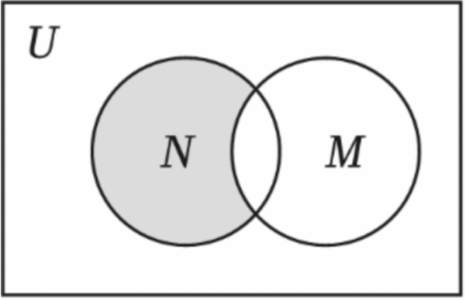
\includegraphics[width=0.30\textwidth]{figures/gao90_q6_venn.png}
\end{center}

\ifanswer
\ans{$N\cap\overline M$}
\fi

\item 已知 $a\in\R$，若关于 $x$ 的方程 $x^2-2x+a-2=0$ 有两个实根 $x_1$、$x_2$，且 $\dfrac1{x_1}+\dfrac1{x_2}=-\dfrac12$，则 $a$ 的值为\blankline[4.4em].

\ifanswer
\solbegin
\step{由于 $x_1$、$x_2$ 是 $x^2-2x+a-2=0$ 的两个实根，}
\step{由韦达定理得 $x_1x_2=a-2$，$x_1+x_2=2$，}
\step{因此 $\dfrac1{x_1}+\dfrac1{x_2}=\dfrac{x_1+x_2}{x_1x_2}=\dfrac2{a-2}=-\dfrac12$，所以 $a-2=-4$，解得 $a=-2$，}
\step{判别式 $\Delta=(-2)^2-4(a-2)=-4a+12$，当 $a=-2$ 时，$\Delta=8+12=20>0$，有两个实根，符合条件，故 $a=-2$.}
\solend
\fi

\item 如果 $-1<x<4$，$-6<y<2$，则 $2x-y$ 的取值范围是\blankline[4.4em].

\ifanswer
\solbegin
\step{因为 $-1<x<4$，$-6<y<2$，所以 $-2<2x<8$，$-2<-y<6$，}
\step{则 $-2+(-2)<2x-y<8+6$，即 $-4<2x-y<14$，}
\step{故 $2x-y$ 的取值范围为 $(-4,14)$.}
\solend
\fi

\item 集合 $A=\left\{x\left|\dfrac6{3-x}\in\Z,x\in\N\right.\right\}$，试用列举法表示集合 $A=\blankline[4.4em]$.

\ifanswer
\solbegin
\step{集合 $A=\left\{x\left|\dfrac6{3-x}\in\Z,x\in\N\right.\right\}$，所以 $3-x$ 可取的值有 $\pm1$、$\pm2$、$\pm3$、$\pm6$，}
\step{又因为 $x\in\N$，所以 $x\in\{0,1,2,4,5,6,9\}$，即 $A=\{0,1,2,4,5,6,9\}$.}
\solend
\fi

\item 不等式 $x^2-ax-b<0$ 的解集是 $(2,3)$，若关于 $x$ 的不等式组 $\begin{cases}(x-a)(3x+b)<0\\ x>t\end{cases}$ 没有实数解，则实数 $t$ 的取值范围是\blankline[4.4em].

\ifanswer
\solbegin
\step{因为等式 $x^2-ax-b<0$ 的解集是 $(2,3)$，所以 $x^2-ax-b=0$ 的根为 $2$、$3$，}
\step{所以 $2+3=a$，$2\times3=-b$，所以 $a=5$，$b=-6$，}
\step{由 $(x-a)(3x+b)=(x-5)(3x-6)<0$ 得 $2<x<5$，}
\step{若关于 $x$ 的不等式组 $\begin{cases}(x-a)(3x+b)<0\\ x>t\end{cases}$ 没有实数解，则 $t\geqslant5$.}
\solend
\fi

\item 若方程 $x^2+2x-m=0$ 有解，则 $m\geqslant a$ 为真命题，则 $a$ 的取值范围为\blankline[4.4em].

\ifanswer
\solbegin
\step{因为方程 $x^2+2x-m=0$ 有解，}
\step{所以 $\Delta=2^2-4\times1\times(-m)=4+4m\geqslant0$，解得 $m\geqslant-1$，}
\step{命题“若方程有解，则 $m\geqslant a$”为真命题，即 $\forall m\in[-1,+\infty)$，$m\geqslant a$ 恒成立，}
\step{因此 $a$ 的取值不能超过集合 $[-1,+\infty)$ 的最小值，即 $a\leqslant-1$，}
\step{综上，$a$ 的取值范围为 $(-\infty,-1]$.}
\solend
\fi

\item 设数集 $M=\left\{x\left|m\leqslant x\leqslant m+\dfrac45\right.\right\}$，$N=\left\{x\left|n-\dfrac14\leqslant x\leqslant n\right.\right\}$，且集合 $M$、$N$ 都是集合 $U=\{x\mid0\leqslant x\leqslant1\}$ 的子集，如果把 $b-a$ 称为非空集合 $\{x\mid a\leqslant x\leqslant b\}$ 的“长度”，那么集合 $M\cap N$ 的“长度”的取值范围为\blankline[4.4em].

\ifanswer
\solbegin
\step{注意到集合 $M$ 的长度为 $\dfrac45$，集合 $N$ 的长度为 $\dfrac14$，均为定值，}
\step{要使得 $M\cap N$ 的“长度”最小，则 $M$ 和 $N$ 尽可能分散到区间的两边，}
\step{长度最小为 $\dfrac45+\dfrac14-1=\dfrac1{20}$；}
\step{要使得 $M\cap N$ 的“长度”最大，则 $M$ 和 $N$ 尽可能集中，}
\step{长度最大就是集合 $N$ 的长度，为 $\dfrac14$，}
\step{故集合 $M\cap N$ 的“长度”的取值范围为 $\left[\dfrac1{20},\dfrac14\right]$.}
\solend
\fi

\end{enumerate}

\bigsec{二、选择题}

\begin{enumerate}
\setcounter{enumi}{12}

\item 设集合 $A=\{x\mid x=2k+1,k\in\Z\}$，$B=\{x\mid x=2k-1,k\in\Z\}$，则 $A$、$B$ 之间的关系是\mbox{（\quad）}

\keepwithprev
A. $B\subsetneq A$\qquad B. $A\subsetneq B$\qquad C. $A=B$\qquad D. 以上都不是

\ifanswer
\solbegin
\step{因为 $k\in\Z$，所以 $2k+1$ 与 $2k-1$ 均表示全体奇数，}
\step{即集合 $A=\{x\mid x=2k+1,k\in\Z\}$ 与 $B=\{x\mid x=2k-1,k\in\Z\}$}
\step{都表示全体奇数构成的集合，所以 $A=B$. 故选 $C$.}
\solend
\fi

\item 已知 $a$、$b\in\R$，且 $a>b$，则下列不等式中一定成立的是\mbox{（\quad）}

\keepwithprev
A. $a+1>b$\qquad B. $a>b+1$\qquad C. $a+1<b+1$\qquad D. $a-1<b-1$

\ifanswer
\solbegin
\step{因为 $a>b$，所以 $a+1>b+1$，$a-1>b-1$，故 $CD$ 错误；}
\step{因为 $a>b$，所以 $a+1>b+0$，即 $a+1>b$ 恒成立，故 $A$ 正确；}
\step{取 $a=1$，$b=0$，$B$ 显然错误.}
\step{故选 $A$.}
\solend
\fi

\item 设 $a$、$b\in\R$，“$a+b>2$ 且 $ab>1$”是“$a>1$，$b>1$”的\mbox{（\quad）}

\keepwithprev
A. 充分不必要条件\qquad B. 必要不充分条件

C. 充要条件\qquad D. 既不充分又不必要条件

\ifanswer
\solbegin
\step{因为 $a>1$ 且 $b>1$，所以 $a+b>2$ 且 $ab>1$，}
\step{若已知 $a+b>2$ 且 $ab>1$，可取 $a=\dfrac12$，$b=8$，也满足已知，}
\step{所以“$a+b>2$ 且 $ab>1$”是“$a>1$ 且 $b>1$”的必要不充分条件，故选 $B$.}
\solend
\fi

\item 设集合 $P_1=\{x\mid x^2+ax+1>0\}$，$P_2=\{x\mid x^2+ax+2>0\}$，$Q_1=\{x\mid x^2+x+b>0\}$，$Q_2=\{x\mid x^2+2x+b>0\}$，其中 $a$、$b\in\R$，下列说法中正确的是\mbox{（\quad）}

\keepwithprev
A. 对任意 $a$，$P_1$ 是 $P_2$ 的子集，对任意 $b$，$Q_1$ 不是 $Q_2$ 的子集

B. 对任意 $a$，$P_1$ 是 $P_2$ 的子集，存在 $b$，使得 $Q_1$ 是 $Q_2$ 的子集

C. 存在 $a$，使得 $P_1$ 不是 $P_2$ 的子集，对任意 $b$，$Q_1$ 不是 $Q_2$ 的子集

D. 存在 $a$，使得 $P_1$ 不是 $P_2$ 的子集，存在 $b$，使得 $Q_1$ 是 $Q_2$ 的子集

\ifanswer
\solbegin
\step{对于集合 $P_1=\{x\mid x^2+ax+1>0\}$，$P_2=\{x\mid x^2+ax+2>0\}$，}
\step{得当 $m\in P_1$ 时，即 $m^2+am+1>0$，得 $m^2+am+2>0$，}
\step{即有 $m\in P_2$，得对任意 $a$，$P_1$ 是 $P_2$ 的子集，}
\step{对于集合 $Q_1=\{x\mid x^2+x+b>0\}$，$Q_2=\{x\mid x^2+2x+b>0\}$，}
\step{当 $b=6$ 时，$Q_1=\{x\mid x^2+x+6>0\}=\R$，$Q_2=\{x\mid x^2+2x+6>0\}=\R$，}
\step{得 $Q_1$ 是 $Q_2$ 的子集，}
\step{当 $b=1$ 时，$Q_1=\{x\mid x^2+x+1>0\}=\R$，}
\step{$Q_2=\{x\mid x^2+2x+1>0\}=\{x\mid x\neq-1\}$，得 $Q_1$ 不是 $Q_2$ 的子集，}
\step{所以存在 $b$，使得 $Q_1$ 是 $Q_2$ 的子集，故选 $B$.}
\solend
\fi

\end{enumerate}

\bigsec{三、解答题}

\begin{enumerate}
\setcounter{enumi}{16}

\item 若 $a$、$b\in\R$，求关于 $x$ 的不等式 $ax\geqslant b$ 的解集.

\ansspace*[9]

\ifanswer
\solbegin
\step{当 $a>0$ 时，原不等式的解集为 $\left\{x\left|x\geqslant\dfrac ba\right.\right\}$；}
\step{当 $a<0$ 时，原不等式的解集为 $\left\{x\left|x\leqslant\dfrac ba\right.\right\}$；}
\step{当 $a=0$，$b\leqslant0$ 时，原不等式的解集为 $\R$；}
\step{当 $a=0$，$b>0$ 时，原不等式的解集为 $\varnothing$.}
\solend
\fi

\item 设集合 $A=\{x\mid x^2+3x+2=0\}$，$B=\{x\mid x^2+(m+1)x+m=0\}$.

（1）用列举法表示集合 $A$；

（2）若 $B\subseteq A$，求实数 $m$ 的值.

\ansspace*[9]

\ifanswer
\solbegin
\stepm{（1）}{集合 $A=\{x\mid x^2+3x+2=0\}$，解方程 $x^2+3x+2=0$，得 $x_1=-2$，$x_2=-1$，}
\step{所以 $A=\{-2,-1\}$.}
\stepm{（2）}{$A=\{-2,-1\}$，$B=\{x\mid x^2+(m+1)x+m=0\}=\{x\mid(x+1)(x+m)=0\}$，}
\step{$B\subseteq A$，所以 $m=1$ 或 $m=2$，所以实数 $m$ 的值为 $1$ 或 $2$.}
\solend
\fi

\item （1）设 $a$、$b$ 是两个正数. 已知 $a>b$，比较 $\dfrac{2a+b}{a+2b}$ 与 $\dfrac ab$ 的值的大小.

（2）用反证法证明：若 $a$、$b\in\R$，且 $x=a^2-2b+1$，$y=b^2-2a+1$，则 $x$、$y$ 中至少有一个不小于 $0$.

\ansspace*[12]

\ifanswer
\solbegin
\stepm{（1）}{$\dfrac{2a+b}{a+2b}-\dfrac ab=\dfrac{b(2a+b)}{b(a+2b)}-\dfrac{a(a+2b)}{b(a+2b)}=\dfrac{b(2a+b)-a(a+2b)}{b(a+2b)}$}
\step{$=\dfrac{2ab+b^2-a^2-2ab}{b(a+2b)}=\dfrac{b^2-a^2}{b(a+2b)}=\dfrac{(b+a)(b-a)}{b(a+2b)}$，}
\step{又 $a>0$，$b>0$，$a>b$，所以 $b+a>0$，$b-a<0$，$b(a+2b)>0$，}
\step{所以 $\dfrac{(b+a)(b-a)}{b(a+2b)}<0$，即 $\dfrac{2a+b}{a+2b}-\dfrac ab<0$，所以 $\dfrac{2a+b}{a+2b}<\dfrac ab$.}
\stepm{（2）}{假设 $x$、$y$ 都小于 $0$，则有 $x+y<0$，}
\step{因为 $x=a^2-2b+1$，$y=b^2-2a+1$，}
\step{所以 $x+y=(a^2-2b+1)+(b^2-2a+1)=(a^2-2a+1)+(b^2-2b+1)$}
\step{$=(a-1)^2+(b-1)^2$，}
\step{又 $a$、$b\in\R$，所以 $(a-1)^2\geqslant0$，$(b-1)^2\geqslant0$，即 $x+y\geqslant0$，}
\step{这与 $x+y<0$ 矛盾，故假设不成立，所以 $x$、$y$ 中至少有一个不小于 $0$.}
\solend
\fi

\item 已知 $m>0$，$p:(x+1)(x-5)\leqslant0$，$q:1-m\leqslant x\leqslant1+m$.

（1）若 $m=5$，$p$、$q$ 有且只有一个为真命题，求实数 $x$ 的取值范围；

（2）若 $p$ 是 $q$ 的充分不必要条件，求实数 $m$ 的取值范围.

\ansspace*[12]

\ifanswer
\solbegin
\stepm{（1）}{对于 $p:(x+1)(x-5)\leqslant0$，解得 $-1\leqslant x\leqslant5$，}
\step{若 $m=5$，则 $q:-4\leqslant x\leqslant6$，}
\step{若 $m=5$，$p$、$q$ 有且只有一个为真命题，则 $p$ 真 $q$ 假或 $p$ 假 $q$ 真，}
\step{若 $p$ 真 $q$ 假，即 $\begin{cases}-1\leqslant x\leqslant5\\ x<-4\ \text{或}\ x>6\end{cases}$，无解，}
\step{若 $p$ 假 $q$ 真，即 $\begin{cases}x<-1\ \text{或}\ x>5\\ -4\leqslant x\leqslant6\end{cases}$，解得 $-4\leqslant x<-1$ 或 $5<x\leqslant6$，}
\step{综上，$-4\leqslant x<-1$ 或 $5<x\leqslant6$，即 $x$ 的取值范围为 $[-4,-1)\cup(5,6]$；}
\stepm{（2）}{若 $p$ 是 $q$ 的充分条件，则有 $\begin{cases}1-m\leqslant-1\\ 5\leqslant1+m\end{cases}$，解得 $m\geqslant4$，}
\step{即 $m$ 的取值范围为 $[4,+\infty)$.}
\solend
\fi

\item 已知关于 $x$ 的不等式：$ax^2-(a+1)x+1<0(a\in\R)$.

（1）当 $a=-2$ 时，求不等式的解集；

（2）当 $a\geqslant0$ 时，求不等式的解集；

（3）命题 $P$：若二次不等式 $ax^2-(a+1)x+1<0$ 的解集为空集，命题 $Q:x^2-2x-a^2+a+1>0$ 对任意实数 $x$ 都成立，若 $P$、$Q$ 中至少有一个真命题，求实数 $a$ 的取值范围.

\ansspace*[14]

\ifanswer
\solbegin
\stepm{（1）}{当 $a=-2$ 时，原不等式为 $2x^2-x-1>0$，即 $(x-1)(2x+1)>0$，}
\step{解得 $x<-\dfrac12$ 或 $x>1$，所以原不等式的解集为 $\left(-\infty,-\dfrac12\right)\cup(1,+\infty)$.}
\stepm{（2）}{当 $a=0$ 时，原不等式为 $-x+1<0$，解得 $x>1$；}
\step{当 $a>0$ 时，原不等式变为 $(ax-1)(x-1)<0$，其对应方程的两根为 $\dfrac1a$，$1$，}
\step{若 $\dfrac1a<1$，即 $a>1$ 时，由 $(ax-1)(x-1)<0$ 解得 $\dfrac1a<x<1$，}
\step{若 $\dfrac1a=1$，即 $a=1$ 时，不等式 $(ax-1)(x-1)<0$ 解集为 $\varnothing$，}
\step{若 $\dfrac1a>1$，即 $0<a<1$ 时，由 $(ax-1)(x-1)<0$ 解得 $1<x<\dfrac1a$，}
\step{综上，当 $a=0$ 时，不等式的解集为 $(1,+\infty)$，}
\step{当 $0<a<1$ 时，不等式的解集为 $\left(1,\dfrac1a\right)$，}
\step{当 $a=1$ 时，不等式的解集为 $\varnothing$，}
\step{当 $a>1$ 时，不等式的解集为 $\left(\dfrac1a,1\right)$.}
\stepm{（3）}{若命题 $P$ 为真命题，}
\step{若 $a<0$，原不等式变为 $(ax-1)(x-1)<0$，其对应方程的两根为 $\dfrac1a$，$1$，}
\step{其解集为 $\left(-\infty,\dfrac1a\right)\cup(1,+\infty)$，不合题意，}
\step{当 $a\geqslant0$ 时，由（2）得当 $a=1$ 时，解集为 $\varnothing$，}
\step{所以命题 $P$ 为真命题，则 $a=1$；}
\step{命题 $Q$ 为真命题，则有相应方程的 $\Delta<0$，即 $a^2-a<0$，解得 $0<a<1$；}
\step{所以当命题 $P$、$Q$ 都为假命题时，$\begin{cases}a\leqslant0\ \text{或}\ a\geqslant1\\ a\neq1\end{cases}$，解得 $a\leqslant0$ 或 $a>1$，}
\step{所以命题 $P$、$Q$ 中至少有一个真命题，则 $0<a\leqslant1$.}
\step{所以实数 $a$ 的取值范围为 $(0,1]$.}
\solend
\fi

\end{enumerate}

\end{document}
"
% 紧凑版：xelatex "\def\iscompact{1}% 高一90_杨思高级中学_10月月考.tex
%   —— 高一上数学“2026-2027 年杨思高级中学高一上 10 月月考”（讲评版）
% 试卷版：xelatex 高一90_杨思高级中学_10月月考.tex
% 答案版：xelatex "\def\isanswer{1}\input{高一90_杨思高级中学_10月月考.tex}"
% 紧凑版：xelatex "\def\iscompact{1}\input{高一90_杨思高级中学_10月月考.tex}"
%
% 原始材料：微信公众号“魔都数学加油站”文章，连载“27学年高一90”；
% 原文标题“27学年高一90——2026-2027年上海市杨思高级中学高一上10月月考”；
% 原文链接：https://mp.weixin.qq.com/s/pvQC5fkWu5Jj3C7dF3-Exw。
% 正文为 8 张 PNG 页（`原图/高一90_杨思高级中学_10月月考/01..08.png`），
% 尺寸混排（第 1、6 页为 2560×3620，其余为 4762×6735），均按页序读取。
%
% 篇幅与题号：原卷自第 3 题起编号（第 1、2 题不在原文内）。填空题 3—12（10 题）、
% 选择题 13—16（4 题）、解答题 17—21（5 题），共 19 题。
%
% 讲评版：第 6 题只印【答案】（“$N\cap\overline M$”），本稿只给 \ans{}；
% 其余 18 题印【解析】，其中选择题答案在解析末句“故选 C／A／B／B”。
% 第 6 题题干带一幅韦恩图（全集 $U$、集合 $M$、$N$ 与阴影部分），三版都出。
%
% 副标题：原卷未印副标题。本稿按内容标作“集合与常用逻辑用语、不等式”。
%
% 原卷笔误/存疑（均照录未改，正文对应处另有 % 注）：
%   ① 第 6 题的韦恩图阴影为 $N$ 中不属于 $M$ 的部分，与所印答案 $N\cap\overline M$ 一致；
%      图与答案均照录。原卷把“（请用各集合的交，并，补表示）”的逗号排作全角逗号，照录；
%   ② 第 12 题题干“如果把 $b-a$ 称为非空集合 $\{x\mid a\leqslant x\leqslant b\}$ 的‘长度’”
%      与本稿统一后的 $\R$、$\Z$、$\N$ 记号无关，原文用斜体 $R$、$Z$、$N$，按惯例改写。
%
% 与原卷的排版差异：
%   ① 原卷每题下直接印【答案】/【解析】，本稿按全稿惯例将答案与解析置于答案版；
%   ② 原卷未印副标题，本稿补出；填空横线统一排 \blankline[4.4em]；
%   ③ 原卷数集记号排斜体 $R$、$Z$、$N$，本稿按全稿惯例改用 $\R$、$\Z$、$\N$；
%   ④ 第 17—21 题的子问用行内“（1）（2）（3）”段，解析中的子问标号用 \stepm；
%   ⑤ 解答题按惯例加 \ansspace；选择题括号排 \mbox{（\quad）}；
%   ⑥ 第 6 题的韦恩图原卷排在题干右侧、文字绕排，本稿改排为题干后的居中图
%      （自原图裁切、去粉色水印后转灰度）。
%
% 行数核对：逐题数 \step/\stepm 条数，合计 94 条（Q3：2；Q4：2；Q5：1；Q6：0；
% Q7：4；Q8：3；Q9：2；Q10：4；Q11：5；Q12：6；Q13：3；Q14：4；Q15：3；Q16：9；
% Q17：4；Q18：4；Q19：10；Q20：8；Q21：20）。第 6 题只印【答案】，不计入 \step 账。
% 原卷解析的换行按语意合并，未逐行强拆。
%
\documentclass[a4paper,11pt]{article}
\usepackage{common}

\begin{document}

\examtitlest[7]{2026--2027 年杨思高级中学高一上 10 月月考}{集合与常用逻辑用语、不等式}

\bigsec{一、填空题}

\begin{enumerate}
\setcounter{enumi}{2}

\item 已知集合 $A=\{x\mid6x+a>0\}$，若 $1\notin A$，则实数 $a$ 的取值范围是\blankline[4.4em].

\ifanswer
\solbegin
\step{集合 $A=\{x\mid6x+a>0\}$，若 $1\notin A$，则 $6+a\leqslant0$ 恒成立，故 $a\leqslant-6$，}
\step{故实数 $a$ 的取值范围是 $(-\infty,-6]$.}
\solend
\fi

\item 设全集 $U=\R$，集合 $A=\{x\mid-1\leqslant x\leqslant1\}$，$B=\{x\mid0<x<2\}$，则 $\overline{A\cup B}=\blankline[4.4em]$.

\ifanswer
\solbegin
\step{$B=\{x\mid0<x<2\}$，$A=\{x\mid-1\leqslant x\leqslant1\}$，所以 $A\cup B=\{x\mid-1\leqslant x<2\}$，}
\step{又因为全集 $U=\R$，所以 $\overline{A\cup B}=(-\infty,-1)\cup[2,+\infty)$.}
\solend
\fi

\item 集合 $A=\{(x,y)\mid y=-x\}$，$B=\{(x,y)\mid y=2x-4\}$，则 $A\cap B=\blankline[4.4em]$.

\ifanswer
\solbegin
\step{联立 $\begin{cases}y=-x\\ y=2x-4\end{cases}$，解得 $\begin{cases}x=\dfrac43\\[0.2em] y=-\dfrac43\end{cases}$，即 $A\cap B=\left\{\left(\dfrac43,-\dfrac43\right)\right\}$.}
\solend
\fi

\item 设 $U$ 是全集，$M$、$N$ 是 $U$ 的子集，则图中阴影部分所表示的集合是\blankline[4.4em].

（请用各集合的交，并，补表示）

\begin{center}
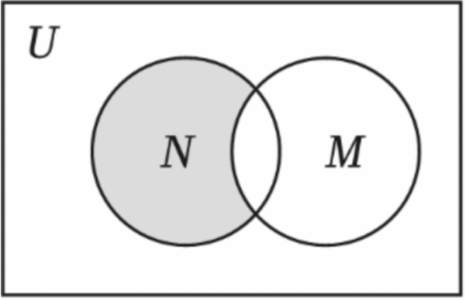
\includegraphics[width=0.30\textwidth]{figures/gao90_q6_venn.png}
\end{center}

\ifanswer
\ans{$N\cap\overline M$}
\fi

\item 已知 $a\in\R$，若关于 $x$ 的方程 $x^2-2x+a-2=0$ 有两个实根 $x_1$、$x_2$，且 $\dfrac1{x_1}+\dfrac1{x_2}=-\dfrac12$，则 $a$ 的值为\blankline[4.4em].

\ifanswer
\solbegin
\step{由于 $x_1$、$x_2$ 是 $x^2-2x+a-2=0$ 的两个实根，}
\step{由韦达定理得 $x_1x_2=a-2$，$x_1+x_2=2$，}
\step{因此 $\dfrac1{x_1}+\dfrac1{x_2}=\dfrac{x_1+x_2}{x_1x_2}=\dfrac2{a-2}=-\dfrac12$，所以 $a-2=-4$，解得 $a=-2$，}
\step{判别式 $\Delta=(-2)^2-4(a-2)=-4a+12$，当 $a=-2$ 时，$\Delta=8+12=20>0$，有两个实根，符合条件，故 $a=-2$.}
\solend
\fi

\item 如果 $-1<x<4$，$-6<y<2$，则 $2x-y$ 的取值范围是\blankline[4.4em].

\ifanswer
\solbegin
\step{因为 $-1<x<4$，$-6<y<2$，所以 $-2<2x<8$，$-2<-y<6$，}
\step{则 $-2+(-2)<2x-y<8+6$，即 $-4<2x-y<14$，}
\step{故 $2x-y$ 的取值范围为 $(-4,14)$.}
\solend
\fi

\item 集合 $A=\left\{x\left|\dfrac6{3-x}\in\Z,x\in\N\right.\right\}$，试用列举法表示集合 $A=\blankline[4.4em]$.

\ifanswer
\solbegin
\step{集合 $A=\left\{x\left|\dfrac6{3-x}\in\Z,x\in\N\right.\right\}$，所以 $3-x$ 可取的值有 $\pm1$、$\pm2$、$\pm3$、$\pm6$，}
\step{又因为 $x\in\N$，所以 $x\in\{0,1,2,4,5,6,9\}$，即 $A=\{0,1,2,4,5,6,9\}$.}
\solend
\fi

\item 不等式 $x^2-ax-b<0$ 的解集是 $(2,3)$，若关于 $x$ 的不等式组 $\begin{cases}(x-a)(3x+b)<0\\ x>t\end{cases}$ 没有实数解，则实数 $t$ 的取值范围是\blankline[4.4em].

\ifanswer
\solbegin
\step{因为等式 $x^2-ax-b<0$ 的解集是 $(2,3)$，所以 $x^2-ax-b=0$ 的根为 $2$、$3$，}
\step{所以 $2+3=a$，$2\times3=-b$，所以 $a=5$，$b=-6$，}
\step{由 $(x-a)(3x+b)=(x-5)(3x-6)<0$ 得 $2<x<5$，}
\step{若关于 $x$ 的不等式组 $\begin{cases}(x-a)(3x+b)<0\\ x>t\end{cases}$ 没有实数解，则 $t\geqslant5$.}
\solend
\fi

\item 若方程 $x^2+2x-m=0$ 有解，则 $m\geqslant a$ 为真命题，则 $a$ 的取值范围为\blankline[4.4em].

\ifanswer
\solbegin
\step{因为方程 $x^2+2x-m=0$ 有解，}
\step{所以 $\Delta=2^2-4\times1\times(-m)=4+4m\geqslant0$，解得 $m\geqslant-1$，}
\step{命题“若方程有解，则 $m\geqslant a$”为真命题，即 $\forall m\in[-1,+\infty)$，$m\geqslant a$ 恒成立，}
\step{因此 $a$ 的取值不能超过集合 $[-1,+\infty)$ 的最小值，即 $a\leqslant-1$，}
\step{综上，$a$ 的取值范围为 $(-\infty,-1]$.}
\solend
\fi

\item 设数集 $M=\left\{x\left|m\leqslant x\leqslant m+\dfrac45\right.\right\}$，$N=\left\{x\left|n-\dfrac14\leqslant x\leqslant n\right.\right\}$，且集合 $M$、$N$ 都是集合 $U=\{x\mid0\leqslant x\leqslant1\}$ 的子集，如果把 $b-a$ 称为非空集合 $\{x\mid a\leqslant x\leqslant b\}$ 的“长度”，那么集合 $M\cap N$ 的“长度”的取值范围为\blankline[4.4em].

\ifanswer
\solbegin
\step{注意到集合 $M$ 的长度为 $\dfrac45$，集合 $N$ 的长度为 $\dfrac14$，均为定值，}
\step{要使得 $M\cap N$ 的“长度”最小，则 $M$ 和 $N$ 尽可能分散到区间的两边，}
\step{长度最小为 $\dfrac45+\dfrac14-1=\dfrac1{20}$；}
\step{要使得 $M\cap N$ 的“长度”最大，则 $M$ 和 $N$ 尽可能集中，}
\step{长度最大就是集合 $N$ 的长度，为 $\dfrac14$，}
\step{故集合 $M\cap N$ 的“长度”的取值范围为 $\left[\dfrac1{20},\dfrac14\right]$.}
\solend
\fi

\end{enumerate}

\bigsec{二、选择题}

\begin{enumerate}
\setcounter{enumi}{12}

\item 设集合 $A=\{x\mid x=2k+1,k\in\Z\}$，$B=\{x\mid x=2k-1,k\in\Z\}$，则 $A$、$B$ 之间的关系是\mbox{（\quad）}

\keepwithprev
A. $B\subsetneq A$\qquad B. $A\subsetneq B$\qquad C. $A=B$\qquad D. 以上都不是

\ifanswer
\solbegin
\step{因为 $k\in\Z$，所以 $2k+1$ 与 $2k-1$ 均表示全体奇数，}
\step{即集合 $A=\{x\mid x=2k+1,k\in\Z\}$ 与 $B=\{x\mid x=2k-1,k\in\Z\}$}
\step{都表示全体奇数构成的集合，所以 $A=B$. 故选 $C$.}
\solend
\fi

\item 已知 $a$、$b\in\R$，且 $a>b$，则下列不等式中一定成立的是\mbox{（\quad）}

\keepwithprev
A. $a+1>b$\qquad B. $a>b+1$\qquad C. $a+1<b+1$\qquad D. $a-1<b-1$

\ifanswer
\solbegin
\step{因为 $a>b$，所以 $a+1>b+1$，$a-1>b-1$，故 $CD$ 错误；}
\step{因为 $a>b$，所以 $a+1>b+0$，即 $a+1>b$ 恒成立，故 $A$ 正确；}
\step{取 $a=1$，$b=0$，$B$ 显然错误.}
\step{故选 $A$.}
\solend
\fi

\item 设 $a$、$b\in\R$，“$a+b>2$ 且 $ab>1$”是“$a>1$，$b>1$”的\mbox{（\quad）}

\keepwithprev
A. 充分不必要条件\qquad B. 必要不充分条件

C. 充要条件\qquad D. 既不充分又不必要条件

\ifanswer
\solbegin
\step{因为 $a>1$ 且 $b>1$，所以 $a+b>2$ 且 $ab>1$，}
\step{若已知 $a+b>2$ 且 $ab>1$，可取 $a=\dfrac12$，$b=8$，也满足已知，}
\step{所以“$a+b>2$ 且 $ab>1$”是“$a>1$ 且 $b>1$”的必要不充分条件，故选 $B$.}
\solend
\fi

\item 设集合 $P_1=\{x\mid x^2+ax+1>0\}$，$P_2=\{x\mid x^2+ax+2>0\}$，$Q_1=\{x\mid x^2+x+b>0\}$，$Q_2=\{x\mid x^2+2x+b>0\}$，其中 $a$、$b\in\R$，下列说法中正确的是\mbox{（\quad）}

\keepwithprev
A. 对任意 $a$，$P_1$ 是 $P_2$ 的子集，对任意 $b$，$Q_1$ 不是 $Q_2$ 的子集

B. 对任意 $a$，$P_1$ 是 $P_2$ 的子集，存在 $b$，使得 $Q_1$ 是 $Q_2$ 的子集

C. 存在 $a$，使得 $P_1$ 不是 $P_2$ 的子集，对任意 $b$，$Q_1$ 不是 $Q_2$ 的子集

D. 存在 $a$，使得 $P_1$ 不是 $P_2$ 的子集，存在 $b$，使得 $Q_1$ 是 $Q_2$ 的子集

\ifanswer
\solbegin
\step{对于集合 $P_1=\{x\mid x^2+ax+1>0\}$，$P_2=\{x\mid x^2+ax+2>0\}$，}
\step{得当 $m\in P_1$ 时，即 $m^2+am+1>0$，得 $m^2+am+2>0$，}
\step{即有 $m\in P_2$，得对任意 $a$，$P_1$ 是 $P_2$ 的子集，}
\step{对于集合 $Q_1=\{x\mid x^2+x+b>0\}$，$Q_2=\{x\mid x^2+2x+b>0\}$，}
\step{当 $b=6$ 时，$Q_1=\{x\mid x^2+x+6>0\}=\R$，$Q_2=\{x\mid x^2+2x+6>0\}=\R$，}
\step{得 $Q_1$ 是 $Q_2$ 的子集，}
\step{当 $b=1$ 时，$Q_1=\{x\mid x^2+x+1>0\}=\R$，}
\step{$Q_2=\{x\mid x^2+2x+1>0\}=\{x\mid x\neq-1\}$，得 $Q_1$ 不是 $Q_2$ 的子集，}
\step{所以存在 $b$，使得 $Q_1$ 是 $Q_2$ 的子集，故选 $B$.}
\solend
\fi

\end{enumerate}

\bigsec{三、解答题}

\begin{enumerate}
\setcounter{enumi}{16}

\item 若 $a$、$b\in\R$，求关于 $x$ 的不等式 $ax\geqslant b$ 的解集.

\ansspace*[9]

\ifanswer
\solbegin
\step{当 $a>0$ 时，原不等式的解集为 $\left\{x\left|x\geqslant\dfrac ba\right.\right\}$；}
\step{当 $a<0$ 时，原不等式的解集为 $\left\{x\left|x\leqslant\dfrac ba\right.\right\}$；}
\step{当 $a=0$，$b\leqslant0$ 时，原不等式的解集为 $\R$；}
\step{当 $a=0$，$b>0$ 时，原不等式的解集为 $\varnothing$.}
\solend
\fi

\item 设集合 $A=\{x\mid x^2+3x+2=0\}$，$B=\{x\mid x^2+(m+1)x+m=0\}$.

（1）用列举法表示集合 $A$；

（2）若 $B\subseteq A$，求实数 $m$ 的值.

\ansspace*[9]

\ifanswer
\solbegin
\stepm{（1）}{集合 $A=\{x\mid x^2+3x+2=0\}$，解方程 $x^2+3x+2=0$，得 $x_1=-2$，$x_2=-1$，}
\step{所以 $A=\{-2,-1\}$.}
\stepm{（2）}{$A=\{-2,-1\}$，$B=\{x\mid x^2+(m+1)x+m=0\}=\{x\mid(x+1)(x+m)=0\}$，}
\step{$B\subseteq A$，所以 $m=1$ 或 $m=2$，所以实数 $m$ 的值为 $1$ 或 $2$.}
\solend
\fi

\item （1）设 $a$、$b$ 是两个正数. 已知 $a>b$，比较 $\dfrac{2a+b}{a+2b}$ 与 $\dfrac ab$ 的值的大小.

（2）用反证法证明：若 $a$、$b\in\R$，且 $x=a^2-2b+1$，$y=b^2-2a+1$，则 $x$、$y$ 中至少有一个不小于 $0$.

\ansspace*[12]

\ifanswer
\solbegin
\stepm{（1）}{$\dfrac{2a+b}{a+2b}-\dfrac ab=\dfrac{b(2a+b)}{b(a+2b)}-\dfrac{a(a+2b)}{b(a+2b)}=\dfrac{b(2a+b)-a(a+2b)}{b(a+2b)}$}
\step{$=\dfrac{2ab+b^2-a^2-2ab}{b(a+2b)}=\dfrac{b^2-a^2}{b(a+2b)}=\dfrac{(b+a)(b-a)}{b(a+2b)}$，}
\step{又 $a>0$，$b>0$，$a>b$，所以 $b+a>0$，$b-a<0$，$b(a+2b)>0$，}
\step{所以 $\dfrac{(b+a)(b-a)}{b(a+2b)}<0$，即 $\dfrac{2a+b}{a+2b}-\dfrac ab<0$，所以 $\dfrac{2a+b}{a+2b}<\dfrac ab$.}
\stepm{（2）}{假设 $x$、$y$ 都小于 $0$，则有 $x+y<0$，}
\step{因为 $x=a^2-2b+1$，$y=b^2-2a+1$，}
\step{所以 $x+y=(a^2-2b+1)+(b^2-2a+1)=(a^2-2a+1)+(b^2-2b+1)$}
\step{$=(a-1)^2+(b-1)^2$，}
\step{又 $a$、$b\in\R$，所以 $(a-1)^2\geqslant0$，$(b-1)^2\geqslant0$，即 $x+y\geqslant0$，}
\step{这与 $x+y<0$ 矛盾，故假设不成立，所以 $x$、$y$ 中至少有一个不小于 $0$.}
\solend
\fi

\item 已知 $m>0$，$p:(x+1)(x-5)\leqslant0$，$q:1-m\leqslant x\leqslant1+m$.

（1）若 $m=5$，$p$、$q$ 有且只有一个为真命题，求实数 $x$ 的取值范围；

（2）若 $p$ 是 $q$ 的充分不必要条件，求实数 $m$ 的取值范围.

\ansspace*[12]

\ifanswer
\solbegin
\stepm{（1）}{对于 $p:(x+1)(x-5)\leqslant0$，解得 $-1\leqslant x\leqslant5$，}
\step{若 $m=5$，则 $q:-4\leqslant x\leqslant6$，}
\step{若 $m=5$，$p$、$q$ 有且只有一个为真命题，则 $p$ 真 $q$ 假或 $p$ 假 $q$ 真，}
\step{若 $p$ 真 $q$ 假，即 $\begin{cases}-1\leqslant x\leqslant5\\ x<-4\ \text{或}\ x>6\end{cases}$，无解，}
\step{若 $p$ 假 $q$ 真，即 $\begin{cases}x<-1\ \text{或}\ x>5\\ -4\leqslant x\leqslant6\end{cases}$，解得 $-4\leqslant x<-1$ 或 $5<x\leqslant6$，}
\step{综上，$-4\leqslant x<-1$ 或 $5<x\leqslant6$，即 $x$ 的取值范围为 $[-4,-1)\cup(5,6]$；}
\stepm{（2）}{若 $p$ 是 $q$ 的充分条件，则有 $\begin{cases}1-m\leqslant-1\\ 5\leqslant1+m\end{cases}$，解得 $m\geqslant4$，}
\step{即 $m$ 的取值范围为 $[4,+\infty)$.}
\solend
\fi

\item 已知关于 $x$ 的不等式：$ax^2-(a+1)x+1<0(a\in\R)$.

（1）当 $a=-2$ 时，求不等式的解集；

（2）当 $a\geqslant0$ 时，求不等式的解集；

（3）命题 $P$：若二次不等式 $ax^2-(a+1)x+1<0$ 的解集为空集，命题 $Q:x^2-2x-a^2+a+1>0$ 对任意实数 $x$ 都成立，若 $P$、$Q$ 中至少有一个真命题，求实数 $a$ 的取值范围.

\ansspace*[14]

\ifanswer
\solbegin
\stepm{（1）}{当 $a=-2$ 时，原不等式为 $2x^2-x-1>0$，即 $(x-1)(2x+1)>0$，}
\step{解得 $x<-\dfrac12$ 或 $x>1$，所以原不等式的解集为 $\left(-\infty,-\dfrac12\right)\cup(1,+\infty)$.}
\stepm{（2）}{当 $a=0$ 时，原不等式为 $-x+1<0$，解得 $x>1$；}
\step{当 $a>0$ 时，原不等式变为 $(ax-1)(x-1)<0$，其对应方程的两根为 $\dfrac1a$，$1$，}
\step{若 $\dfrac1a<1$，即 $a>1$ 时，由 $(ax-1)(x-1)<0$ 解得 $\dfrac1a<x<1$，}
\step{若 $\dfrac1a=1$，即 $a=1$ 时，不等式 $(ax-1)(x-1)<0$ 解集为 $\varnothing$，}
\step{若 $\dfrac1a>1$，即 $0<a<1$ 时，由 $(ax-1)(x-1)<0$ 解得 $1<x<\dfrac1a$，}
\step{综上，当 $a=0$ 时，不等式的解集为 $(1,+\infty)$，}
\step{当 $0<a<1$ 时，不等式的解集为 $\left(1,\dfrac1a\right)$，}
\step{当 $a=1$ 时，不等式的解集为 $\varnothing$，}
\step{当 $a>1$ 时，不等式的解集为 $\left(\dfrac1a,1\right)$.}
\stepm{（3）}{若命题 $P$ 为真命题，}
\step{若 $a<0$，原不等式变为 $(ax-1)(x-1)<0$，其对应方程的两根为 $\dfrac1a$，$1$，}
\step{其解集为 $\left(-\infty,\dfrac1a\right)\cup(1,+\infty)$，不合题意，}
\step{当 $a\geqslant0$ 时，由（2）得当 $a=1$ 时，解集为 $\varnothing$，}
\step{所以命题 $P$ 为真命题，则 $a=1$；}
\step{命题 $Q$ 为真命题，则有相应方程的 $\Delta<0$，即 $a^2-a<0$，解得 $0<a<1$；}
\step{所以当命题 $P$、$Q$ 都为假命题时，$\begin{cases}a\leqslant0\ \text{或}\ a\geqslant1\\ a\neq1\end{cases}$，解得 $a\leqslant0$ 或 $a>1$，}
\step{所以命题 $P$、$Q$ 中至少有一个真命题，则 $0<a\leqslant1$.}
\step{所以实数 $a$ 的取值范围为 $(0,1]$.}
\solend
\fi

\end{enumerate}

\end{document}
"
%
% 原始材料：微信公众号“魔都数学加油站”文章，连载“27学年高一90”；
% 原文标题“27学年高一90——2026-2027年上海市杨思高级中学高一上10月月考”；
% 原文链接：https://mp.weixin.qq.com/s/pvQC5fkWu5Jj3C7dF3-Exw。
% 正文为 8 张 PNG 页（`原图/高一90_杨思高级中学_10月月考/01..08.png`），
% 尺寸混排（第 1、6 页为 2560×3620，其余为 4762×6735），均按页序读取。
%
% 篇幅与题号：原卷自第 3 题起编号（第 1、2 题不在原文内）。填空题 3—12（10 题）、
% 选择题 13—16（4 题）、解答题 17—21（5 题），共 19 题。
%
% 讲评版：第 6 题只印【答案】（“$N\cap\overline M$”），本稿只给 \ans{}；
% 其余 18 题印【解析】，其中选择题答案在解析末句“故选 C／A／B／B”。
% 第 6 题题干带一幅韦恩图（全集 $U$、集合 $M$、$N$ 与阴影部分），三版都出。
%
% 副标题：原卷未印副标题。本稿按内容标作“集合与常用逻辑用语、不等式”。
%
% 原卷笔误/存疑（均照录未改，正文对应处另有 % 注）：
%   ① 第 6 题的韦恩图阴影为 $N$ 中不属于 $M$ 的部分，与所印答案 $N\cap\overline M$ 一致；
%      图与答案均照录。原卷把“（请用各集合的交，并，补表示）”的逗号排作全角逗号，照录；
%   ② 第 12 题题干“如果把 $b-a$ 称为非空集合 $\{x\mid a\leqslant x\leqslant b\}$ 的‘长度’”
%      与本稿统一后的 $\R$、$\Z$、$\N$ 记号无关，原文用斜体 $R$、$Z$、$N$，按惯例改写。
%
% 与原卷的排版差异：
%   ① 原卷每题下直接印【答案】/【解析】，本稿按全稿惯例将答案与解析置于答案版；
%   ② 原卷未印副标题，本稿补出；填空横线统一排 \blankline[4.4em]；
%   ③ 原卷数集记号排斜体 $R$、$Z$、$N$，本稿按全稿惯例改用 $\R$、$\Z$、$\N$；
%   ④ 第 17—21 题的子问用行内“（1）（2）（3）”段，解析中的子问标号用 \stepm；
%   ⑤ 解答题按惯例加 \ansspace；选择题括号排 \mbox{（\quad）}；
%   ⑥ 第 6 题的韦恩图原卷排在题干右侧、文字绕排，本稿改排为题干后的居中图
%      （自原图裁切、去粉色水印后转灰度）。
%
% 行数核对：逐题数 \step/\stepm 条数，合计 94 条（Q3：2；Q4：2；Q5：1；Q6：0；
% Q7：4；Q8：3；Q9：2；Q10：4；Q11：5；Q12：6；Q13：3；Q14：4；Q15：3；Q16：9；
% Q17：4；Q18：4；Q19：10；Q20：8；Q21：20）。第 6 题只印【答案】，不计入 \step 账。
% 原卷解析的换行按语意合并，未逐行强拆。
%
\documentclass[a4paper,11pt]{article}
\usepackage{common}

\begin{document}

\examtitlest[7]{2026--2027 年杨思高级中学高一上 10 月月考}{集合与常用逻辑用语、不等式}

\bigsec{一、填空题}

\begin{enumerate}
\setcounter{enumi}{2}

\item 已知集合 $A=\{x\mid6x+a>0\}$，若 $1\notin A$，则实数 $a$ 的取值范围是\blankline[4.4em].

\ifanswer
\solbegin
\step{集合 $A=\{x\mid6x+a>0\}$，若 $1\notin A$，则 $6+a\leqslant0$ 恒成立，故 $a\leqslant-6$，}
\step{故实数 $a$ 的取值范围是 $(-\infty,-6]$.}
\solend
\fi

\item 设全集 $U=\R$，集合 $A=\{x\mid-1\leqslant x\leqslant1\}$，$B=\{x\mid0<x<2\}$，则 $\overline{A\cup B}=\blankline[4.4em]$.

\ifanswer
\solbegin
\step{$B=\{x\mid0<x<2\}$，$A=\{x\mid-1\leqslant x\leqslant1\}$，所以 $A\cup B=\{x\mid-1\leqslant x<2\}$，}
\step{又因为全集 $U=\R$，所以 $\overline{A\cup B}=(-\infty,-1)\cup[2,+\infty)$.}
\solend
\fi

\item 集合 $A=\{(x,y)\mid y=-x\}$，$B=\{(x,y)\mid y=2x-4\}$，则 $A\cap B=\blankline[4.4em]$.

\ifanswer
\solbegin
\step{联立 $\begin{cases}y=-x\\ y=2x-4\end{cases}$，解得 $\begin{cases}x=\dfrac43\\[0.2em] y=-\dfrac43\end{cases}$，即 $A\cap B=\left\{\left(\dfrac43,-\dfrac43\right)\right\}$.}
\solend
\fi

\item 设 $U$ 是全集，$M$、$N$ 是 $U$ 的子集，则图中阴影部分所表示的集合是\blankline[4.4em].

（请用各集合的交，并，补表示）

\begin{center}
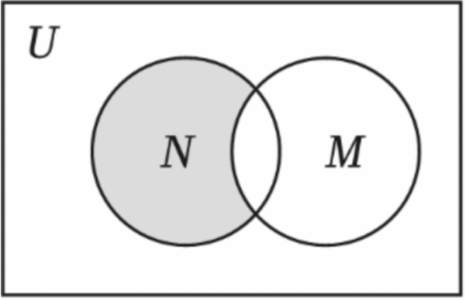
\includegraphics[width=0.30\textwidth]{figures/gao90_q6_venn.png}
\end{center}

\ifanswer
\ans{$N\cap\overline M$}
\fi

\item 已知 $a\in\R$，若关于 $x$ 的方程 $x^2-2x+a-2=0$ 有两个实根 $x_1$、$x_2$，且 $\dfrac1{x_1}+\dfrac1{x_2}=-\dfrac12$，则 $a$ 的值为\blankline[4.4em].

\ifanswer
\solbegin
\step{由于 $x_1$、$x_2$ 是 $x^2-2x+a-2=0$ 的两个实根，}
\step{由韦达定理得 $x_1x_2=a-2$，$x_1+x_2=2$，}
\step{因此 $\dfrac1{x_1}+\dfrac1{x_2}=\dfrac{x_1+x_2}{x_1x_2}=\dfrac2{a-2}=-\dfrac12$，所以 $a-2=-4$，解得 $a=-2$，}
\step{判别式 $\Delta=(-2)^2-4(a-2)=-4a+12$，当 $a=-2$ 时，$\Delta=8+12=20>0$，有两个实根，符合条件，故 $a=-2$.}
\solend
\fi

\item 如果 $-1<x<4$，$-6<y<2$，则 $2x-y$ 的取值范围是\blankline[4.4em].

\ifanswer
\solbegin
\step{因为 $-1<x<4$，$-6<y<2$，所以 $-2<2x<8$，$-2<-y<6$，}
\step{则 $-2+(-2)<2x-y<8+6$，即 $-4<2x-y<14$，}
\step{故 $2x-y$ 的取值范围为 $(-4,14)$.}
\solend
\fi

\item 集合 $A=\left\{x\left|\dfrac6{3-x}\in\Z,x\in\N\right.\right\}$，试用列举法表示集合 $A=\blankline[4.4em]$.

\ifanswer
\solbegin
\step{集合 $A=\left\{x\left|\dfrac6{3-x}\in\Z,x\in\N\right.\right\}$，所以 $3-x$ 可取的值有 $\pm1$、$\pm2$、$\pm3$、$\pm6$，}
\step{又因为 $x\in\N$，所以 $x\in\{0,1,2,4,5,6,9\}$，即 $A=\{0,1,2,4,5,6,9\}$.}
\solend
\fi

\item 不等式 $x^2-ax-b<0$ 的解集是 $(2,3)$，若关于 $x$ 的不等式组 $\begin{cases}(x-a)(3x+b)<0\\ x>t\end{cases}$ 没有实数解，则实数 $t$ 的取值范围是\blankline[4.4em].

\ifanswer
\solbegin
\step{因为等式 $x^2-ax-b<0$ 的解集是 $(2,3)$，所以 $x^2-ax-b=0$ 的根为 $2$、$3$，}
\step{所以 $2+3=a$，$2\times3=-b$，所以 $a=5$，$b=-6$，}
\step{由 $(x-a)(3x+b)=(x-5)(3x-6)<0$ 得 $2<x<5$，}
\step{若关于 $x$ 的不等式组 $\begin{cases}(x-a)(3x+b)<0\\ x>t\end{cases}$ 没有实数解，则 $t\geqslant5$.}
\solend
\fi

\item 若方程 $x^2+2x-m=0$ 有解，则 $m\geqslant a$ 为真命题，则 $a$ 的取值范围为\blankline[4.4em].

\ifanswer
\solbegin
\step{因为方程 $x^2+2x-m=0$ 有解，}
\step{所以 $\Delta=2^2-4\times1\times(-m)=4+4m\geqslant0$，解得 $m\geqslant-1$，}
\step{命题“若方程有解，则 $m\geqslant a$”为真命题，即 $\forall m\in[-1,+\infty)$，$m\geqslant a$ 恒成立，}
\step{因此 $a$ 的取值不能超过集合 $[-1,+\infty)$ 的最小值，即 $a\leqslant-1$，}
\step{综上，$a$ 的取值范围为 $(-\infty,-1]$.}
\solend
\fi

\item 设数集 $M=\left\{x\left|m\leqslant x\leqslant m+\dfrac45\right.\right\}$，$N=\left\{x\left|n-\dfrac14\leqslant x\leqslant n\right.\right\}$，且集合 $M$、$N$ 都是集合 $U=\{x\mid0\leqslant x\leqslant1\}$ 的子集，如果把 $b-a$ 称为非空集合 $\{x\mid a\leqslant x\leqslant b\}$ 的“长度”，那么集合 $M\cap N$ 的“长度”的取值范围为\blankline[4.4em].

\ifanswer
\solbegin
\step{注意到集合 $M$ 的长度为 $\dfrac45$，集合 $N$ 的长度为 $\dfrac14$，均为定值，}
\step{要使得 $M\cap N$ 的“长度”最小，则 $M$ 和 $N$ 尽可能分散到区间的两边，}
\step{长度最小为 $\dfrac45+\dfrac14-1=\dfrac1{20}$；}
\step{要使得 $M\cap N$ 的“长度”最大，则 $M$ 和 $N$ 尽可能集中，}
\step{长度最大就是集合 $N$ 的长度，为 $\dfrac14$，}
\step{故集合 $M\cap N$ 的“长度”的取值范围为 $\left[\dfrac1{20},\dfrac14\right]$.}
\solend
\fi

\end{enumerate}

\bigsec{二、选择题}

\begin{enumerate}
\setcounter{enumi}{12}

\item 设集合 $A=\{x\mid x=2k+1,k\in\Z\}$，$B=\{x\mid x=2k-1,k\in\Z\}$，则 $A$、$B$ 之间的关系是\mbox{（\quad）}

\keepwithprev
A. $B\subsetneq A$\qquad B. $A\subsetneq B$\qquad C. $A=B$\qquad D. 以上都不是

\ifanswer
\solbegin
\step{因为 $k\in\Z$，所以 $2k+1$ 与 $2k-1$ 均表示全体奇数，}
\step{即集合 $A=\{x\mid x=2k+1,k\in\Z\}$ 与 $B=\{x\mid x=2k-1,k\in\Z\}$}
\step{都表示全体奇数构成的集合，所以 $A=B$. 故选 $C$.}
\solend
\fi

\item 已知 $a$、$b\in\R$，且 $a>b$，则下列不等式中一定成立的是\mbox{（\quad）}

\keepwithprev
A. $a+1>b$\qquad B. $a>b+1$\qquad C. $a+1<b+1$\qquad D. $a-1<b-1$

\ifanswer
\solbegin
\step{因为 $a>b$，所以 $a+1>b+1$，$a-1>b-1$，故 $CD$ 错误；}
\step{因为 $a>b$，所以 $a+1>b+0$，即 $a+1>b$ 恒成立，故 $A$ 正确；}
\step{取 $a=1$，$b=0$，$B$ 显然错误.}
\step{故选 $A$.}
\solend
\fi

\item 设 $a$、$b\in\R$，“$a+b>2$ 且 $ab>1$”是“$a>1$，$b>1$”的\mbox{（\quad）}

\keepwithprev
A. 充分不必要条件\qquad B. 必要不充分条件

C. 充要条件\qquad D. 既不充分又不必要条件

\ifanswer
\solbegin
\step{因为 $a>1$ 且 $b>1$，所以 $a+b>2$ 且 $ab>1$，}
\step{若已知 $a+b>2$ 且 $ab>1$，可取 $a=\dfrac12$，$b=8$，也满足已知，}
\step{所以“$a+b>2$ 且 $ab>1$”是“$a>1$ 且 $b>1$”的必要不充分条件，故选 $B$.}
\solend
\fi

\item 设集合 $P_1=\{x\mid x^2+ax+1>0\}$，$P_2=\{x\mid x^2+ax+2>0\}$，$Q_1=\{x\mid x^2+x+b>0\}$，$Q_2=\{x\mid x^2+2x+b>0\}$，其中 $a$、$b\in\R$，下列说法中正确的是\mbox{（\quad）}

\keepwithprev
A. 对任意 $a$，$P_1$ 是 $P_2$ 的子集，对任意 $b$，$Q_1$ 不是 $Q_2$ 的子集

B. 对任意 $a$，$P_1$ 是 $P_2$ 的子集，存在 $b$，使得 $Q_1$ 是 $Q_2$ 的子集

C. 存在 $a$，使得 $P_1$ 不是 $P_2$ 的子集，对任意 $b$，$Q_1$ 不是 $Q_2$ 的子集

D. 存在 $a$，使得 $P_1$ 不是 $P_2$ 的子集，存在 $b$，使得 $Q_1$ 是 $Q_2$ 的子集

\ifanswer
\solbegin
\step{对于集合 $P_1=\{x\mid x^2+ax+1>0\}$，$P_2=\{x\mid x^2+ax+2>0\}$，}
\step{得当 $m\in P_1$ 时，即 $m^2+am+1>0$，得 $m^2+am+2>0$，}
\step{即有 $m\in P_2$，得对任意 $a$，$P_1$ 是 $P_2$ 的子集，}
\step{对于集合 $Q_1=\{x\mid x^2+x+b>0\}$，$Q_2=\{x\mid x^2+2x+b>0\}$，}
\step{当 $b=6$ 时，$Q_1=\{x\mid x^2+x+6>0\}=\R$，$Q_2=\{x\mid x^2+2x+6>0\}=\R$，}
\step{得 $Q_1$ 是 $Q_2$ 的子集，}
\step{当 $b=1$ 时，$Q_1=\{x\mid x^2+x+1>0\}=\R$，}
\step{$Q_2=\{x\mid x^2+2x+1>0\}=\{x\mid x\neq-1\}$，得 $Q_1$ 不是 $Q_2$ 的子集，}
\step{所以存在 $b$，使得 $Q_1$ 是 $Q_2$ 的子集，故选 $B$.}
\solend
\fi

\end{enumerate}

\bigsec{三、解答题}

\begin{enumerate}
\setcounter{enumi}{16}

\item 若 $a$、$b\in\R$，求关于 $x$ 的不等式 $ax\geqslant b$ 的解集.

\ansspace*[9]

\ifanswer
\solbegin
\step{当 $a>0$ 时，原不等式的解集为 $\left\{x\left|x\geqslant\dfrac ba\right.\right\}$；}
\step{当 $a<0$ 时，原不等式的解集为 $\left\{x\left|x\leqslant\dfrac ba\right.\right\}$；}
\step{当 $a=0$，$b\leqslant0$ 时，原不等式的解集为 $\R$；}
\step{当 $a=0$，$b>0$ 时，原不等式的解集为 $\varnothing$.}
\solend
\fi

\item 设集合 $A=\{x\mid x^2+3x+2=0\}$，$B=\{x\mid x^2+(m+1)x+m=0\}$.

（1）用列举法表示集合 $A$；

（2）若 $B\subseteq A$，求实数 $m$ 的值.

\ansspace*[9]

\ifanswer
\solbegin
\stepm{（1）}{集合 $A=\{x\mid x^2+3x+2=0\}$，解方程 $x^2+3x+2=0$，得 $x_1=-2$，$x_2=-1$，}
\step{所以 $A=\{-2,-1\}$.}
\stepm{（2）}{$A=\{-2,-1\}$，$B=\{x\mid x^2+(m+1)x+m=0\}=\{x\mid(x+1)(x+m)=0\}$，}
\step{$B\subseteq A$，所以 $m=1$ 或 $m=2$，所以实数 $m$ 的值为 $1$ 或 $2$.}
\solend
\fi

\item （1）设 $a$、$b$ 是两个正数. 已知 $a>b$，比较 $\dfrac{2a+b}{a+2b}$ 与 $\dfrac ab$ 的值的大小.

（2）用反证法证明：若 $a$、$b\in\R$，且 $x=a^2-2b+1$，$y=b^2-2a+1$，则 $x$、$y$ 中至少有一个不小于 $0$.

\ansspace*[12]

\ifanswer
\solbegin
\stepm{（1）}{$\dfrac{2a+b}{a+2b}-\dfrac ab=\dfrac{b(2a+b)}{b(a+2b)}-\dfrac{a(a+2b)}{b(a+2b)}=\dfrac{b(2a+b)-a(a+2b)}{b(a+2b)}$}
\step{$=\dfrac{2ab+b^2-a^2-2ab}{b(a+2b)}=\dfrac{b^2-a^2}{b(a+2b)}=\dfrac{(b+a)(b-a)}{b(a+2b)}$，}
\step{又 $a>0$，$b>0$，$a>b$，所以 $b+a>0$，$b-a<0$，$b(a+2b)>0$，}
\step{所以 $\dfrac{(b+a)(b-a)}{b(a+2b)}<0$，即 $\dfrac{2a+b}{a+2b}-\dfrac ab<0$，所以 $\dfrac{2a+b}{a+2b}<\dfrac ab$.}
\stepm{（2）}{假设 $x$、$y$ 都小于 $0$，则有 $x+y<0$，}
\step{因为 $x=a^2-2b+1$，$y=b^2-2a+1$，}
\step{所以 $x+y=(a^2-2b+1)+(b^2-2a+1)=(a^2-2a+1)+(b^2-2b+1)$}
\step{$=(a-1)^2+(b-1)^2$，}
\step{又 $a$、$b\in\R$，所以 $(a-1)^2\geqslant0$，$(b-1)^2\geqslant0$，即 $x+y\geqslant0$，}
\step{这与 $x+y<0$ 矛盾，故假设不成立，所以 $x$、$y$ 中至少有一个不小于 $0$.}
\solend
\fi

\item 已知 $m>0$，$p:(x+1)(x-5)\leqslant0$，$q:1-m\leqslant x\leqslant1+m$.

（1）若 $m=5$，$p$、$q$ 有且只有一个为真命题，求实数 $x$ 的取值范围；

（2）若 $p$ 是 $q$ 的充分不必要条件，求实数 $m$ 的取值范围.

\ansspace*[12]

\ifanswer
\solbegin
\stepm{（1）}{对于 $p:(x+1)(x-5)\leqslant0$，解得 $-1\leqslant x\leqslant5$，}
\step{若 $m=5$，则 $q:-4\leqslant x\leqslant6$，}
\step{若 $m=5$，$p$、$q$ 有且只有一个为真命题，则 $p$ 真 $q$ 假或 $p$ 假 $q$ 真，}
\step{若 $p$ 真 $q$ 假，即 $\begin{cases}-1\leqslant x\leqslant5\\ x<-4\ \text{或}\ x>6\end{cases}$，无解，}
\step{若 $p$ 假 $q$ 真，即 $\begin{cases}x<-1\ \text{或}\ x>5\\ -4\leqslant x\leqslant6\end{cases}$，解得 $-4\leqslant x<-1$ 或 $5<x\leqslant6$，}
\step{综上，$-4\leqslant x<-1$ 或 $5<x\leqslant6$，即 $x$ 的取值范围为 $[-4,-1)\cup(5,6]$；}
\stepm{（2）}{若 $p$ 是 $q$ 的充分条件，则有 $\begin{cases}1-m\leqslant-1\\ 5\leqslant1+m\end{cases}$，解得 $m\geqslant4$，}
\step{即 $m$ 的取值范围为 $[4,+\infty)$.}
\solend
\fi

\item 已知关于 $x$ 的不等式：$ax^2-(a+1)x+1<0(a\in\R)$.

（1）当 $a=-2$ 时，求不等式的解集；

（2）当 $a\geqslant0$ 时，求不等式的解集；

（3）命题 $P$：若二次不等式 $ax^2-(a+1)x+1<0$ 的解集为空集，命题 $Q:x^2-2x-a^2+a+1>0$ 对任意实数 $x$ 都成立，若 $P$、$Q$ 中至少有一个真命题，求实数 $a$ 的取值范围.

\ansspace*[14]

\ifanswer
\solbegin
\stepm{（1）}{当 $a=-2$ 时，原不等式为 $2x^2-x-1>0$，即 $(x-1)(2x+1)>0$，}
\step{解得 $x<-\dfrac12$ 或 $x>1$，所以原不等式的解集为 $\left(-\infty,-\dfrac12\right)\cup(1,+\infty)$.}
\stepm{（2）}{当 $a=0$ 时，原不等式为 $-x+1<0$，解得 $x>1$；}
\step{当 $a>0$ 时，原不等式变为 $(ax-1)(x-1)<0$，其对应方程的两根为 $\dfrac1a$，$1$，}
\step{若 $\dfrac1a<1$，即 $a>1$ 时，由 $(ax-1)(x-1)<0$ 解得 $\dfrac1a<x<1$，}
\step{若 $\dfrac1a=1$，即 $a=1$ 时，不等式 $(ax-1)(x-1)<0$ 解集为 $\varnothing$，}
\step{若 $\dfrac1a>1$，即 $0<a<1$ 时，由 $(ax-1)(x-1)<0$ 解得 $1<x<\dfrac1a$，}
\step{综上，当 $a=0$ 时，不等式的解集为 $(1,+\infty)$，}
\step{当 $0<a<1$ 时，不等式的解集为 $\left(1,\dfrac1a\right)$，}
\step{当 $a=1$ 时，不等式的解集为 $\varnothing$，}
\step{当 $a>1$ 时，不等式的解集为 $\left(\dfrac1a,1\right)$.}
\stepm{（3）}{若命题 $P$ 为真命题，}
\step{若 $a<0$，原不等式变为 $(ax-1)(x-1)<0$，其对应方程的两根为 $\dfrac1a$，$1$，}
\step{其解集为 $\left(-\infty,\dfrac1a\right)\cup(1,+\infty)$，不合题意，}
\step{当 $a\geqslant0$ 时，由（2）得当 $a=1$ 时，解集为 $\varnothing$，}
\step{所以命题 $P$ 为真命题，则 $a=1$；}
\step{命题 $Q$ 为真命题，则有相应方程的 $\Delta<0$，即 $a^2-a<0$，解得 $0<a<1$；}
\step{所以当命题 $P$、$Q$ 都为假命题时，$\begin{cases}a\leqslant0\ \text{或}\ a\geqslant1\\ a\neq1\end{cases}$，解得 $a\leqslant0$ 或 $a>1$，}
\step{所以命题 $P$、$Q$ 中至少有一个真命题，则 $0<a\leqslant1$.}
\step{所以实数 $a$ 的取值范围为 $(0,1]$.}
\solend
\fi

\end{enumerate}

\end{document}
"
%
% 原始材料：微信公众号“魔都数学加油站”文章，连载“27学年高一90”；
% 原文标题“27学年高一90——2026-2027年上海市杨思高级中学高一上10月月考”；
% 原文链接：https://mp.weixin.qq.com/s/pvQC5fkWu5Jj3C7dF3-Exw。
% 正文为 8 张 PNG 页（`原图/高一90_杨思高级中学_10月月考/01..08.png`），
% 尺寸混排（第 1、6 页为 2560×3620，其余为 4762×6735），均按页序读取。
%
% 篇幅与题号：原卷自第 3 题起编号（第 1、2 题不在原文内）。填空题 3—12（10 题）、
% 选择题 13—16（4 题）、解答题 17—21（5 题），共 19 题。
%
% 讲评版：第 6 题只印【答案】（“$N\cap\overline M$”），本稿只给 \ans{}；
% 其余 18 题印【解析】，其中选择题答案在解析末句“故选 C／A／B／B”。
% 第 6 题题干带一幅韦恩图（全集 $U$、集合 $M$、$N$ 与阴影部分），三版都出。
%
% 副标题：原卷未印副标题。本稿按内容标作“集合与常用逻辑用语、不等式”。
%
% 原卷笔误/存疑（均照录未改，正文对应处另有 % 注）：
%   ① 第 6 题的韦恩图阴影为 $N$ 中不属于 $M$ 的部分，与所印答案 $N\cap\overline M$ 一致；
%      图与答案均照录。原卷把“（请用各集合的交，并，补表示）”的逗号排作全角逗号，照录；
%   ② 第 12 题题干“如果把 $b-a$ 称为非空集合 $\{x\mid a\leqslant x\leqslant b\}$ 的‘长度’”
%      与本稿统一后的 $\R$、$\Z$、$\N$ 记号无关，原文用斜体 $R$、$Z$、$N$，按惯例改写。
%
% 与原卷的排版差异：
%   ① 原卷每题下直接印【答案】/【解析】，本稿按全稿惯例将答案与解析置于答案版；
%   ② 原卷未印副标题，本稿补出；填空横线统一排 \blankline[4.4em]；
%   ③ 原卷数集记号排斜体 $R$、$Z$、$N$，本稿按全稿惯例改用 $\R$、$\Z$、$\N$；
%   ④ 第 17—21 题的子问用行内“（1）（2）（3）”段，解析中的子问标号用 \stepm；
%   ⑤ 解答题按惯例加 \ansspace；选择题括号排 \mbox{（\quad）}；
%   ⑥ 第 6 题的韦恩图原卷排在题干右侧、文字绕排，本稿改排为题干后的居中图
%      （自原图裁切、去粉色水印后转灰度）。
%
% 行数核对：逐题数 \step/\stepm 条数，合计 94 条（Q3：2；Q4：2；Q5：1；Q6：0；
% Q7：4；Q8：3；Q9：2；Q10：4；Q11：5；Q12：6；Q13：3；Q14：4；Q15：3；Q16：9；
% Q17：4；Q18：4；Q19：10；Q20：8；Q21：20）。第 6 题只印【答案】，不计入 \step 账。
% 原卷解析的换行按语意合并，未逐行强拆。
%
\documentclass[a4paper,11pt]{article}
\usepackage{common}

\begin{document}

\examtitlest[7]{2026--2027 年杨思高级中学高一上 10 月月考}{集合与常用逻辑用语、不等式}

\bigsec{一、填空题}

\begin{enumerate}
\setcounter{enumi}{2}

\item 已知集合 $A=\{x\mid6x+a>0\}$，若 $1\notin A$，则实数 $a$ 的取值范围是\blankline[4.4em].

\ifanswer
\solbegin
\step{集合 $A=\{x\mid6x+a>0\}$，若 $1\notin A$，则 $6+a\leqslant0$ 恒成立，故 $a\leqslant-6$，}
\step{故实数 $a$ 的取值范围是 $(-\infty,-6]$.}
\solend
\fi

\item 设全集 $U=\R$，集合 $A=\{x\mid-1\leqslant x\leqslant1\}$，$B=\{x\mid0<x<2\}$，则 $\overline{A\cup B}=\blankline[4.4em]$.

\ifanswer
\solbegin
\step{$B=\{x\mid0<x<2\}$，$A=\{x\mid-1\leqslant x\leqslant1\}$，所以 $A\cup B=\{x\mid-1\leqslant x<2\}$，}
\step{又因为全集 $U=\R$，所以 $\overline{A\cup B}=(-\infty,-1)\cup[2,+\infty)$.}
\solend
\fi

\item 集合 $A=\{(x,y)\mid y=-x\}$，$B=\{(x,y)\mid y=2x-4\}$，则 $A\cap B=\blankline[4.4em]$.

\ifanswer
\solbegin
\step{联立 $\begin{cases}y=-x\\ y=2x-4\end{cases}$，解得 $\begin{cases}x=\dfrac43\\[0.2em] y=-\dfrac43\end{cases}$，即 $A\cap B=\left\{\left(\dfrac43,-\dfrac43\right)\right\}$.}
\solend
\fi

\item 设 $U$ 是全集，$M$、$N$ 是 $U$ 的子集，则图中阴影部分所表示的集合是\blankline[4.4em].

（请用各集合的交，并，补表示）

\begin{center}
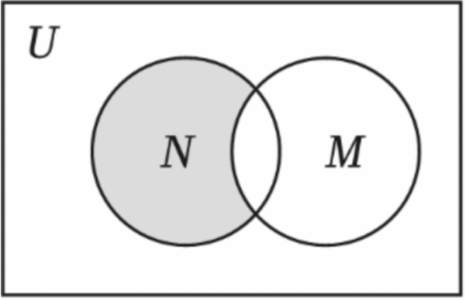
\includegraphics[width=0.30\textwidth]{figures/gao90_q6_venn.png}
\end{center}

\ifanswer
\ans{$N\cap\overline M$}
\fi

\item 已知 $a\in\R$，若关于 $x$ 的方程 $x^2-2x+a-2=0$ 有两个实根 $x_1$、$x_2$，且 $\dfrac1{x_1}+\dfrac1{x_2}=-\dfrac12$，则 $a$ 的值为\blankline[4.4em].

\ifanswer
\solbegin
\step{由于 $x_1$、$x_2$ 是 $x^2-2x+a-2=0$ 的两个实根，}
\step{由韦达定理得 $x_1x_2=a-2$，$x_1+x_2=2$，}
\step{因此 $\dfrac1{x_1}+\dfrac1{x_2}=\dfrac{x_1+x_2}{x_1x_2}=\dfrac2{a-2}=-\dfrac12$，所以 $a-2=-4$，解得 $a=-2$，}
\step{判别式 $\Delta=(-2)^2-4(a-2)=-4a+12$，当 $a=-2$ 时，$\Delta=8+12=20>0$，有两个实根，符合条件，故 $a=-2$.}
\solend
\fi

\item 如果 $-1<x<4$，$-6<y<2$，则 $2x-y$ 的取值范围是\blankline[4.4em].

\ifanswer
\solbegin
\step{因为 $-1<x<4$，$-6<y<2$，所以 $-2<2x<8$，$-2<-y<6$，}
\step{则 $-2+(-2)<2x-y<8+6$，即 $-4<2x-y<14$，}
\step{故 $2x-y$ 的取值范围为 $(-4,14)$.}
\solend
\fi

\item 集合 $A=\left\{x\left|\dfrac6{3-x}\in\Z,x\in\N\right.\right\}$，试用列举法表示集合 $A=\blankline[4.4em]$.

\ifanswer
\solbegin
\step{集合 $A=\left\{x\left|\dfrac6{3-x}\in\Z,x\in\N\right.\right\}$，所以 $3-x$ 可取的值有 $\pm1$、$\pm2$、$\pm3$、$\pm6$，}
\step{又因为 $x\in\N$，所以 $x\in\{0,1,2,4,5,6,9\}$，即 $A=\{0,1,2,4,5,6,9\}$.}
\solend
\fi

\item 不等式 $x^2-ax-b<0$ 的解集是 $(2,3)$，若关于 $x$ 的不等式组 $\begin{cases}(x-a)(3x+b)<0\\ x>t\end{cases}$ 没有实数解，则实数 $t$ 的取值范围是\blankline[4.4em].

\ifanswer
\solbegin
\step{因为等式 $x^2-ax-b<0$ 的解集是 $(2,3)$，所以 $x^2-ax-b=0$ 的根为 $2$、$3$，}
\step{所以 $2+3=a$，$2\times3=-b$，所以 $a=5$，$b=-6$，}
\step{由 $(x-a)(3x+b)=(x-5)(3x-6)<0$ 得 $2<x<5$，}
\step{若关于 $x$ 的不等式组 $\begin{cases}(x-a)(3x+b)<0\\ x>t\end{cases}$ 没有实数解，则 $t\geqslant5$.}
\solend
\fi

\item 若方程 $x^2+2x-m=0$ 有解，则 $m\geqslant a$ 为真命题，则 $a$ 的取值范围为\blankline[4.4em].

\ifanswer
\solbegin
\step{因为方程 $x^2+2x-m=0$ 有解，}
\step{所以 $\Delta=2^2-4\times1\times(-m)=4+4m\geqslant0$，解得 $m\geqslant-1$，}
\step{命题“若方程有解，则 $m\geqslant a$”为真命题，即 $\forall m\in[-1,+\infty)$，$m\geqslant a$ 恒成立，}
\step{因此 $a$ 的取值不能超过集合 $[-1,+\infty)$ 的最小值，即 $a\leqslant-1$，}
\step{综上，$a$ 的取值范围为 $(-\infty,-1]$.}
\solend
\fi

\item 设数集 $M=\left\{x\left|m\leqslant x\leqslant m+\dfrac45\right.\right\}$，$N=\left\{x\left|n-\dfrac14\leqslant x\leqslant n\right.\right\}$，且集合 $M$、$N$ 都是集合 $U=\{x\mid0\leqslant x\leqslant1\}$ 的子集，如果把 $b-a$ 称为非空集合 $\{x\mid a\leqslant x\leqslant b\}$ 的“长度”，那么集合 $M\cap N$ 的“长度”的取值范围为\blankline[4.4em].

\ifanswer
\solbegin
\step{注意到集合 $M$ 的长度为 $\dfrac45$，集合 $N$ 的长度为 $\dfrac14$，均为定值，}
\step{要使得 $M\cap N$ 的“长度”最小，则 $M$ 和 $N$ 尽可能分散到区间的两边，}
\step{长度最小为 $\dfrac45+\dfrac14-1=\dfrac1{20}$；}
\step{要使得 $M\cap N$ 的“长度”最大，则 $M$ 和 $N$ 尽可能集中，}
\step{长度最大就是集合 $N$ 的长度，为 $\dfrac14$，}
\step{故集合 $M\cap N$ 的“长度”的取值范围为 $\left[\dfrac1{20},\dfrac14\right]$.}
\solend
\fi

\end{enumerate}

\bigsec{二、选择题}

\begin{enumerate}
\setcounter{enumi}{12}

\item 设集合 $A=\{x\mid x=2k+1,k\in\Z\}$，$B=\{x\mid x=2k-1,k\in\Z\}$，则 $A$、$B$ 之间的关系是\mbox{（\quad）}

\keepwithprev
A. $B\subsetneq A$\qquad B. $A\subsetneq B$\qquad C. $A=B$\qquad D. 以上都不是

\ifanswer
\solbegin
\step{因为 $k\in\Z$，所以 $2k+1$ 与 $2k-1$ 均表示全体奇数，}
\step{即集合 $A=\{x\mid x=2k+1,k\in\Z\}$ 与 $B=\{x\mid x=2k-1,k\in\Z\}$}
\step{都表示全体奇数构成的集合，所以 $A=B$. 故选 $C$.}
\solend
\fi

\item 已知 $a$、$b\in\R$，且 $a>b$，则下列不等式中一定成立的是\mbox{（\quad）}

\keepwithprev
A. $a+1>b$\qquad B. $a>b+1$\qquad C. $a+1<b+1$\qquad D. $a-1<b-1$

\ifanswer
\solbegin
\step{因为 $a>b$，所以 $a+1>b+1$，$a-1>b-1$，故 $CD$ 错误；}
\step{因为 $a>b$，所以 $a+1>b+0$，即 $a+1>b$ 恒成立，故 $A$ 正确；}
\step{取 $a=1$，$b=0$，$B$ 显然错误.}
\step{故选 $A$.}
\solend
\fi

\item 设 $a$、$b\in\R$，“$a+b>2$ 且 $ab>1$”是“$a>1$，$b>1$”的\mbox{（\quad）}

\keepwithprev
A. 充分不必要条件\qquad B. 必要不充分条件

C. 充要条件\qquad D. 既不充分又不必要条件

\ifanswer
\solbegin
\step{因为 $a>1$ 且 $b>1$，所以 $a+b>2$ 且 $ab>1$，}
\step{若已知 $a+b>2$ 且 $ab>1$，可取 $a=\dfrac12$，$b=8$，也满足已知，}
\step{所以“$a+b>2$ 且 $ab>1$”是“$a>1$ 且 $b>1$”的必要不充分条件，故选 $B$.}
\solend
\fi

\item 设集合 $P_1=\{x\mid x^2+ax+1>0\}$，$P_2=\{x\mid x^2+ax+2>0\}$，$Q_1=\{x\mid x^2+x+b>0\}$，$Q_2=\{x\mid x^2+2x+b>0\}$，其中 $a$、$b\in\R$，下列说法中正确的是\mbox{（\quad）}

\keepwithprev
A. 对任意 $a$，$P_1$ 是 $P_2$ 的子集，对任意 $b$，$Q_1$ 不是 $Q_2$ 的子集

B. 对任意 $a$，$P_1$ 是 $P_2$ 的子集，存在 $b$，使得 $Q_1$ 是 $Q_2$ 的子集

C. 存在 $a$，使得 $P_1$ 不是 $P_2$ 的子集，对任意 $b$，$Q_1$ 不是 $Q_2$ 的子集

D. 存在 $a$，使得 $P_1$ 不是 $P_2$ 的子集，存在 $b$，使得 $Q_1$ 是 $Q_2$ 的子集

\ifanswer
\solbegin
\step{对于集合 $P_1=\{x\mid x^2+ax+1>0\}$，$P_2=\{x\mid x^2+ax+2>0\}$，}
\step{得当 $m\in P_1$ 时，即 $m^2+am+1>0$，得 $m^2+am+2>0$，}
\step{即有 $m\in P_2$，得对任意 $a$，$P_1$ 是 $P_2$ 的子集，}
\step{对于集合 $Q_1=\{x\mid x^2+x+b>0\}$，$Q_2=\{x\mid x^2+2x+b>0\}$，}
\step{当 $b=6$ 时，$Q_1=\{x\mid x^2+x+6>0\}=\R$，$Q_2=\{x\mid x^2+2x+6>0\}=\R$，}
\step{得 $Q_1$ 是 $Q_2$ 的子集，}
\step{当 $b=1$ 时，$Q_1=\{x\mid x^2+x+1>0\}=\R$，}
\step{$Q_2=\{x\mid x^2+2x+1>0\}=\{x\mid x\neq-1\}$，得 $Q_1$ 不是 $Q_2$ 的子集，}
\step{所以存在 $b$，使得 $Q_1$ 是 $Q_2$ 的子集，故选 $B$.}
\solend
\fi

\end{enumerate}

\bigsec{三、解答题}

\begin{enumerate}
\setcounter{enumi}{16}

\item 若 $a$、$b\in\R$，求关于 $x$ 的不等式 $ax\geqslant b$ 的解集.

\ansspace*[9]

\ifanswer
\solbegin
\step{当 $a>0$ 时，原不等式的解集为 $\left\{x\left|x\geqslant\dfrac ba\right.\right\}$；}
\step{当 $a<0$ 时，原不等式的解集为 $\left\{x\left|x\leqslant\dfrac ba\right.\right\}$；}
\step{当 $a=0$，$b\leqslant0$ 时，原不等式的解集为 $\R$；}
\step{当 $a=0$，$b>0$ 时，原不等式的解集为 $\varnothing$.}
\solend
\fi

\item 设集合 $A=\{x\mid x^2+3x+2=0\}$，$B=\{x\mid x^2+(m+1)x+m=0\}$.

（1）用列举法表示集合 $A$；

（2）若 $B\subseteq A$，求实数 $m$ 的值.

\ansspace*[9]

\ifanswer
\solbegin
\stepm{（1）}{集合 $A=\{x\mid x^2+3x+2=0\}$，解方程 $x^2+3x+2=0$，得 $x_1=-2$，$x_2=-1$，}
\step{所以 $A=\{-2,-1\}$.}
\stepm{（2）}{$A=\{-2,-1\}$，$B=\{x\mid x^2+(m+1)x+m=0\}=\{x\mid(x+1)(x+m)=0\}$，}
\step{$B\subseteq A$，所以 $m=1$ 或 $m=2$，所以实数 $m$ 的值为 $1$ 或 $2$.}
\solend
\fi

\item （1）设 $a$、$b$ 是两个正数. 已知 $a>b$，比较 $\dfrac{2a+b}{a+2b}$ 与 $\dfrac ab$ 的值的大小.

（2）用反证法证明：若 $a$、$b\in\R$，且 $x=a^2-2b+1$，$y=b^2-2a+1$，则 $x$、$y$ 中至少有一个不小于 $0$.

\ansspace*[12]

\ifanswer
\solbegin
\stepm{（1）}{$\dfrac{2a+b}{a+2b}-\dfrac ab=\dfrac{b(2a+b)}{b(a+2b)}-\dfrac{a(a+2b)}{b(a+2b)}=\dfrac{b(2a+b)-a(a+2b)}{b(a+2b)}$}
\step{$=\dfrac{2ab+b^2-a^2-2ab}{b(a+2b)}=\dfrac{b^2-a^2}{b(a+2b)}=\dfrac{(b+a)(b-a)}{b(a+2b)}$，}
\step{又 $a>0$，$b>0$，$a>b$，所以 $b+a>0$，$b-a<0$，$b(a+2b)>0$，}
\step{所以 $\dfrac{(b+a)(b-a)}{b(a+2b)}<0$，即 $\dfrac{2a+b}{a+2b}-\dfrac ab<0$，所以 $\dfrac{2a+b}{a+2b}<\dfrac ab$.}
\stepm{（2）}{假设 $x$、$y$ 都小于 $0$，则有 $x+y<0$，}
\step{因为 $x=a^2-2b+1$，$y=b^2-2a+1$，}
\step{所以 $x+y=(a^2-2b+1)+(b^2-2a+1)=(a^2-2a+1)+(b^2-2b+1)$}
\step{$=(a-1)^2+(b-1)^2$，}
\step{又 $a$、$b\in\R$，所以 $(a-1)^2\geqslant0$，$(b-1)^2\geqslant0$，即 $x+y\geqslant0$，}
\step{这与 $x+y<0$ 矛盾，故假设不成立，所以 $x$、$y$ 中至少有一个不小于 $0$.}
\solend
\fi

\item 已知 $m>0$，$p:(x+1)(x-5)\leqslant0$，$q:1-m\leqslant x\leqslant1+m$.

（1）若 $m=5$，$p$、$q$ 有且只有一个为真命题，求实数 $x$ 的取值范围；

（2）若 $p$ 是 $q$ 的充分不必要条件，求实数 $m$ 的取值范围.

\ansspace*[12]

\ifanswer
\solbegin
\stepm{（1）}{对于 $p:(x+1)(x-5)\leqslant0$，解得 $-1\leqslant x\leqslant5$，}
\step{若 $m=5$，则 $q:-4\leqslant x\leqslant6$，}
\step{若 $m=5$，$p$、$q$ 有且只有一个为真命题，则 $p$ 真 $q$ 假或 $p$ 假 $q$ 真，}
\step{若 $p$ 真 $q$ 假，即 $\begin{cases}-1\leqslant x\leqslant5\\ x<-4\ \text{或}\ x>6\end{cases}$，无解，}
\step{若 $p$ 假 $q$ 真，即 $\begin{cases}x<-1\ \text{或}\ x>5\\ -4\leqslant x\leqslant6\end{cases}$，解得 $-4\leqslant x<-1$ 或 $5<x\leqslant6$，}
\step{综上，$-4\leqslant x<-1$ 或 $5<x\leqslant6$，即 $x$ 的取值范围为 $[-4,-1)\cup(5,6]$；}
\stepm{（2）}{若 $p$ 是 $q$ 的充分条件，则有 $\begin{cases}1-m\leqslant-1\\ 5\leqslant1+m\end{cases}$，解得 $m\geqslant4$，}
\step{即 $m$ 的取值范围为 $[4,+\infty)$.}
\solend
\fi

\item 已知关于 $x$ 的不等式：$ax^2-(a+1)x+1<0(a\in\R)$.

（1）当 $a=-2$ 时，求不等式的解集；

（2）当 $a\geqslant0$ 时，求不等式的解集；

（3）命题 $P$：若二次不等式 $ax^2-(a+1)x+1<0$ 的解集为空集，命题 $Q:x^2-2x-a^2+a+1>0$ 对任意实数 $x$ 都成立，若 $P$、$Q$ 中至少有一个真命题，求实数 $a$ 的取值范围.

\ansspace*[14]

\ifanswer
\solbegin
\stepm{（1）}{当 $a=-2$ 时，原不等式为 $2x^2-x-1>0$，即 $(x-1)(2x+1)>0$，}
\step{解得 $x<-\dfrac12$ 或 $x>1$，所以原不等式的解集为 $\left(-\infty,-\dfrac12\right)\cup(1,+\infty)$.}
\stepm{（2）}{当 $a=0$ 时，原不等式为 $-x+1<0$，解得 $x>1$；}
\step{当 $a>0$ 时，原不等式变为 $(ax-1)(x-1)<0$，其对应方程的两根为 $\dfrac1a$，$1$，}
\step{若 $\dfrac1a<1$，即 $a>1$ 时，由 $(ax-1)(x-1)<0$ 解得 $\dfrac1a<x<1$，}
\step{若 $\dfrac1a=1$，即 $a=1$ 时，不等式 $(ax-1)(x-1)<0$ 解集为 $\varnothing$，}
\step{若 $\dfrac1a>1$，即 $0<a<1$ 时，由 $(ax-1)(x-1)<0$ 解得 $1<x<\dfrac1a$，}
\step{综上，当 $a=0$ 时，不等式的解集为 $(1,+\infty)$，}
\step{当 $0<a<1$ 时，不等式的解集为 $\left(1,\dfrac1a\right)$，}
\step{当 $a=1$ 时，不等式的解集为 $\varnothing$，}
\step{当 $a>1$ 时，不等式的解集为 $\left(\dfrac1a,1\right)$.}
\stepm{（3）}{若命题 $P$ 为真命题，}
\step{若 $a<0$，原不等式变为 $(ax-1)(x-1)<0$，其对应方程的两根为 $\dfrac1a$，$1$，}
\step{其解集为 $\left(-\infty,\dfrac1a\right)\cup(1,+\infty)$，不合题意，}
\step{当 $a\geqslant0$ 时，由（2）得当 $a=1$ 时，解集为 $\varnothing$，}
\step{所以命题 $P$ 为真命题，则 $a=1$；}
\step{命题 $Q$ 为真命题，则有相应方程的 $\Delta<0$，即 $a^2-a<0$，解得 $0<a<1$；}
\step{所以当命题 $P$、$Q$ 都为假命题时，$\begin{cases}a\leqslant0\ \text{或}\ a\geqslant1\\ a\neq1\end{cases}$，解得 $a\leqslant0$ 或 $a>1$，}
\step{所以命题 $P$、$Q$ 中至少有一个真命题，则 $0<a\leqslant1$.}
\step{所以实数 $a$ 的取值范围为 $(0,1]$.}
\solend
\fi

\end{enumerate}

\end{document}
"
% 紧凑版：xelatex "\def\iscompact{1}% 高一90_杨思高级中学_10月月考.tex
%   —— 高一上数学“2026-2027 年杨思高级中学高一上 10 月月考”（讲评版）
% 试卷版：xelatex 高一90_杨思高级中学_10月月考.tex
% 答案版：xelatex "\def\isanswer{1}% 高一90_杨思高级中学_10月月考.tex
%   —— 高一上数学“2026-2027 年杨思高级中学高一上 10 月月考”（讲评版）
% 试卷版：xelatex 高一90_杨思高级中学_10月月考.tex
% 答案版：xelatex "\def\isanswer{1}% 高一90_杨思高级中学_10月月考.tex
%   —— 高一上数学“2026-2027 年杨思高级中学高一上 10 月月考”（讲评版）
% 试卷版：xelatex 高一90_杨思高级中学_10月月考.tex
% 答案版：xelatex "\def\isanswer{1}\input{高一90_杨思高级中学_10月月考.tex}"
% 紧凑版：xelatex "\def\iscompact{1}\input{高一90_杨思高级中学_10月月考.tex}"
%
% 原始材料：微信公众号“魔都数学加油站”文章，连载“27学年高一90”；
% 原文标题“27学年高一90——2026-2027年上海市杨思高级中学高一上10月月考”；
% 原文链接：https://mp.weixin.qq.com/s/pvQC5fkWu5Jj3C7dF3-Exw。
% 正文为 8 张 PNG 页（`原图/高一90_杨思高级中学_10月月考/01..08.png`），
% 尺寸混排（第 1、6 页为 2560×3620，其余为 4762×6735），均按页序读取。
%
% 篇幅与题号：原卷自第 3 题起编号（第 1、2 题不在原文内）。填空题 3—12（10 题）、
% 选择题 13—16（4 题）、解答题 17—21（5 题），共 19 题。
%
% 讲评版：第 6 题只印【答案】（“$N\cap\overline M$”），本稿只给 \ans{}；
% 其余 18 题印【解析】，其中选择题答案在解析末句“故选 C／A／B／B”。
% 第 6 题题干带一幅韦恩图（全集 $U$、集合 $M$、$N$ 与阴影部分），三版都出。
%
% 副标题：原卷未印副标题。本稿按内容标作“集合与常用逻辑用语、不等式”。
%
% 原卷笔误/存疑（均照录未改，正文对应处另有 % 注）：
%   ① 第 6 题的韦恩图阴影为 $N$ 中不属于 $M$ 的部分，与所印答案 $N\cap\overline M$ 一致；
%      图与答案均照录。原卷把“（请用各集合的交，并，补表示）”的逗号排作全角逗号，照录；
%   ② 第 12 题题干“如果把 $b-a$ 称为非空集合 $\{x\mid a\leqslant x\leqslant b\}$ 的‘长度’”
%      与本稿统一后的 $\R$、$\Z$、$\N$ 记号无关，原文用斜体 $R$、$Z$、$N$，按惯例改写。
%
% 与原卷的排版差异：
%   ① 原卷每题下直接印【答案】/【解析】，本稿按全稿惯例将答案与解析置于答案版；
%   ② 原卷未印副标题，本稿补出；填空横线统一排 \blankline[4.4em]；
%   ③ 原卷数集记号排斜体 $R$、$Z$、$N$，本稿按全稿惯例改用 $\R$、$\Z$、$\N$；
%   ④ 第 17—21 题的子问用行内“（1）（2）（3）”段，解析中的子问标号用 \stepm；
%   ⑤ 解答题按惯例加 \ansspace；选择题括号排 \mbox{（\quad）}；
%   ⑥ 第 6 题的韦恩图原卷排在题干右侧、文字绕排，本稿改排为题干后的居中图
%      （自原图裁切、去粉色水印后转灰度）。
%
% 行数核对：逐题数 \step/\stepm 条数，合计 94 条（Q3：2；Q4：2；Q5：1；Q6：0；
% Q7：4；Q8：3；Q9：2；Q10：4；Q11：5；Q12：6；Q13：3；Q14：4；Q15：3；Q16：9；
% Q17：4；Q18：4；Q19：10；Q20：8；Q21：20）。第 6 题只印【答案】，不计入 \step 账。
% 原卷解析的换行按语意合并，未逐行强拆。
%
\documentclass[a4paper,11pt]{article}
\usepackage{common}

\begin{document}

\examtitlest[7]{2026--2027 年杨思高级中学高一上 10 月月考}{集合与常用逻辑用语、不等式}

\bigsec{一、填空题}

\begin{enumerate}
\setcounter{enumi}{2}

\item 已知集合 $A=\{x\mid6x+a>0\}$，若 $1\notin A$，则实数 $a$ 的取值范围是\blankline[4.4em].

\ifanswer
\solbegin
\step{集合 $A=\{x\mid6x+a>0\}$，若 $1\notin A$，则 $6+a\leqslant0$ 恒成立，故 $a\leqslant-6$，}
\step{故实数 $a$ 的取值范围是 $(-\infty,-6]$.}
\solend
\fi

\item 设全集 $U=\R$，集合 $A=\{x\mid-1\leqslant x\leqslant1\}$，$B=\{x\mid0<x<2\}$，则 $\overline{A\cup B}=\blankline[4.4em]$.

\ifanswer
\solbegin
\step{$B=\{x\mid0<x<2\}$，$A=\{x\mid-1\leqslant x\leqslant1\}$，所以 $A\cup B=\{x\mid-1\leqslant x<2\}$，}
\step{又因为全集 $U=\R$，所以 $\overline{A\cup B}=(-\infty,-1)\cup[2,+\infty)$.}
\solend
\fi

\item 集合 $A=\{(x,y)\mid y=-x\}$，$B=\{(x,y)\mid y=2x-4\}$，则 $A\cap B=\blankline[4.4em]$.

\ifanswer
\solbegin
\step{联立 $\begin{cases}y=-x\\ y=2x-4\end{cases}$，解得 $\begin{cases}x=\dfrac43\\[0.2em] y=-\dfrac43\end{cases}$，即 $A\cap B=\left\{\left(\dfrac43,-\dfrac43\right)\right\}$.}
\solend
\fi

\item 设 $U$ 是全集，$M$、$N$ 是 $U$ 的子集，则图中阴影部分所表示的集合是\blankline[4.4em].

（请用各集合的交，并，补表示）

\begin{center}
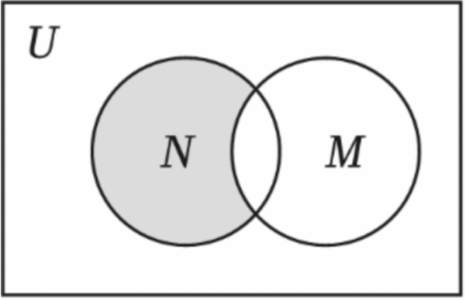
\includegraphics[width=0.30\textwidth]{figures/gao90_q6_venn.png}
\end{center}

\ifanswer
\ans{$N\cap\overline M$}
\fi

\item 已知 $a\in\R$，若关于 $x$ 的方程 $x^2-2x+a-2=0$ 有两个实根 $x_1$、$x_2$，且 $\dfrac1{x_1}+\dfrac1{x_2}=-\dfrac12$，则 $a$ 的值为\blankline[4.4em].

\ifanswer
\solbegin
\step{由于 $x_1$、$x_2$ 是 $x^2-2x+a-2=0$ 的两个实根，}
\step{由韦达定理得 $x_1x_2=a-2$，$x_1+x_2=2$，}
\step{因此 $\dfrac1{x_1}+\dfrac1{x_2}=\dfrac{x_1+x_2}{x_1x_2}=\dfrac2{a-2}=-\dfrac12$，所以 $a-2=-4$，解得 $a=-2$，}
\step{判别式 $\Delta=(-2)^2-4(a-2)=-4a+12$，当 $a=-2$ 时，$\Delta=8+12=20>0$，有两个实根，符合条件，故 $a=-2$.}
\solend
\fi

\item 如果 $-1<x<4$，$-6<y<2$，则 $2x-y$ 的取值范围是\blankline[4.4em].

\ifanswer
\solbegin
\step{因为 $-1<x<4$，$-6<y<2$，所以 $-2<2x<8$，$-2<-y<6$，}
\step{则 $-2+(-2)<2x-y<8+6$，即 $-4<2x-y<14$，}
\step{故 $2x-y$ 的取值范围为 $(-4,14)$.}
\solend
\fi

\item 集合 $A=\left\{x\left|\dfrac6{3-x}\in\Z,x\in\N\right.\right\}$，试用列举法表示集合 $A=\blankline[4.4em]$.

\ifanswer
\solbegin
\step{集合 $A=\left\{x\left|\dfrac6{3-x}\in\Z,x\in\N\right.\right\}$，所以 $3-x$ 可取的值有 $\pm1$、$\pm2$、$\pm3$、$\pm6$，}
\step{又因为 $x\in\N$，所以 $x\in\{0,1,2,4,5,6,9\}$，即 $A=\{0,1,2,4,5,6,9\}$.}
\solend
\fi

\item 不等式 $x^2-ax-b<0$ 的解集是 $(2,3)$，若关于 $x$ 的不等式组 $\begin{cases}(x-a)(3x+b)<0\\ x>t\end{cases}$ 没有实数解，则实数 $t$ 的取值范围是\blankline[4.4em].

\ifanswer
\solbegin
\step{因为等式 $x^2-ax-b<0$ 的解集是 $(2,3)$，所以 $x^2-ax-b=0$ 的根为 $2$、$3$，}
\step{所以 $2+3=a$，$2\times3=-b$，所以 $a=5$，$b=-6$，}
\step{由 $(x-a)(3x+b)=(x-5)(3x-6)<0$ 得 $2<x<5$，}
\step{若关于 $x$ 的不等式组 $\begin{cases}(x-a)(3x+b)<0\\ x>t\end{cases}$ 没有实数解，则 $t\geqslant5$.}
\solend
\fi

\item 若方程 $x^2+2x-m=0$ 有解，则 $m\geqslant a$ 为真命题，则 $a$ 的取值范围为\blankline[4.4em].

\ifanswer
\solbegin
\step{因为方程 $x^2+2x-m=0$ 有解，}
\step{所以 $\Delta=2^2-4\times1\times(-m)=4+4m\geqslant0$，解得 $m\geqslant-1$，}
\step{命题“若方程有解，则 $m\geqslant a$”为真命题，即 $\forall m\in[-1,+\infty)$，$m\geqslant a$ 恒成立，}
\step{因此 $a$ 的取值不能超过集合 $[-1,+\infty)$ 的最小值，即 $a\leqslant-1$，}
\step{综上，$a$ 的取值范围为 $(-\infty,-1]$.}
\solend
\fi

\item 设数集 $M=\left\{x\left|m\leqslant x\leqslant m+\dfrac45\right.\right\}$，$N=\left\{x\left|n-\dfrac14\leqslant x\leqslant n\right.\right\}$，且集合 $M$、$N$ 都是集合 $U=\{x\mid0\leqslant x\leqslant1\}$ 的子集，如果把 $b-a$ 称为非空集合 $\{x\mid a\leqslant x\leqslant b\}$ 的“长度”，那么集合 $M\cap N$ 的“长度”的取值范围为\blankline[4.4em].

\ifanswer
\solbegin
\step{注意到集合 $M$ 的长度为 $\dfrac45$，集合 $N$ 的长度为 $\dfrac14$，均为定值，}
\step{要使得 $M\cap N$ 的“长度”最小，则 $M$ 和 $N$ 尽可能分散到区间的两边，}
\step{长度最小为 $\dfrac45+\dfrac14-1=\dfrac1{20}$；}
\step{要使得 $M\cap N$ 的“长度”最大，则 $M$ 和 $N$ 尽可能集中，}
\step{长度最大就是集合 $N$ 的长度，为 $\dfrac14$，}
\step{故集合 $M\cap N$ 的“长度”的取值范围为 $\left[\dfrac1{20},\dfrac14\right]$.}
\solend
\fi

\end{enumerate}

\bigsec{二、选择题}

\begin{enumerate}
\setcounter{enumi}{12}

\item 设集合 $A=\{x\mid x=2k+1,k\in\Z\}$，$B=\{x\mid x=2k-1,k\in\Z\}$，则 $A$、$B$ 之间的关系是\mbox{（\quad）}

\keepwithprev
A. $B\subsetneq A$\qquad B. $A\subsetneq B$\qquad C. $A=B$\qquad D. 以上都不是

\ifanswer
\solbegin
\step{因为 $k\in\Z$，所以 $2k+1$ 与 $2k-1$ 均表示全体奇数，}
\step{即集合 $A=\{x\mid x=2k+1,k\in\Z\}$ 与 $B=\{x\mid x=2k-1,k\in\Z\}$}
\step{都表示全体奇数构成的集合，所以 $A=B$. 故选 $C$.}
\solend
\fi

\item 已知 $a$、$b\in\R$，且 $a>b$，则下列不等式中一定成立的是\mbox{（\quad）}

\keepwithprev
A. $a+1>b$\qquad B. $a>b+1$\qquad C. $a+1<b+1$\qquad D. $a-1<b-1$

\ifanswer
\solbegin
\step{因为 $a>b$，所以 $a+1>b+1$，$a-1>b-1$，故 $CD$ 错误；}
\step{因为 $a>b$，所以 $a+1>b+0$，即 $a+1>b$ 恒成立，故 $A$ 正确；}
\step{取 $a=1$，$b=0$，$B$ 显然错误.}
\step{故选 $A$.}
\solend
\fi

\item 设 $a$、$b\in\R$，“$a+b>2$ 且 $ab>1$”是“$a>1$，$b>1$”的\mbox{（\quad）}

\keepwithprev
A. 充分不必要条件\qquad B. 必要不充分条件

C. 充要条件\qquad D. 既不充分又不必要条件

\ifanswer
\solbegin
\step{因为 $a>1$ 且 $b>1$，所以 $a+b>2$ 且 $ab>1$，}
\step{若已知 $a+b>2$ 且 $ab>1$，可取 $a=\dfrac12$，$b=8$，也满足已知，}
\step{所以“$a+b>2$ 且 $ab>1$”是“$a>1$ 且 $b>1$”的必要不充分条件，故选 $B$.}
\solend
\fi

\item 设集合 $P_1=\{x\mid x^2+ax+1>0\}$，$P_2=\{x\mid x^2+ax+2>0\}$，$Q_1=\{x\mid x^2+x+b>0\}$，$Q_2=\{x\mid x^2+2x+b>0\}$，其中 $a$、$b\in\R$，下列说法中正确的是\mbox{（\quad）}

\keepwithprev
A. 对任意 $a$，$P_1$ 是 $P_2$ 的子集，对任意 $b$，$Q_1$ 不是 $Q_2$ 的子集

B. 对任意 $a$，$P_1$ 是 $P_2$ 的子集，存在 $b$，使得 $Q_1$ 是 $Q_2$ 的子集

C. 存在 $a$，使得 $P_1$ 不是 $P_2$ 的子集，对任意 $b$，$Q_1$ 不是 $Q_2$ 的子集

D. 存在 $a$，使得 $P_1$ 不是 $P_2$ 的子集，存在 $b$，使得 $Q_1$ 是 $Q_2$ 的子集

\ifanswer
\solbegin
\step{对于集合 $P_1=\{x\mid x^2+ax+1>0\}$，$P_2=\{x\mid x^2+ax+2>0\}$，}
\step{得当 $m\in P_1$ 时，即 $m^2+am+1>0$，得 $m^2+am+2>0$，}
\step{即有 $m\in P_2$，得对任意 $a$，$P_1$ 是 $P_2$ 的子集，}
\step{对于集合 $Q_1=\{x\mid x^2+x+b>0\}$，$Q_2=\{x\mid x^2+2x+b>0\}$，}
\step{当 $b=6$ 时，$Q_1=\{x\mid x^2+x+6>0\}=\R$，$Q_2=\{x\mid x^2+2x+6>0\}=\R$，}
\step{得 $Q_1$ 是 $Q_2$ 的子集，}
\step{当 $b=1$ 时，$Q_1=\{x\mid x^2+x+1>0\}=\R$，}
\step{$Q_2=\{x\mid x^2+2x+1>0\}=\{x\mid x\neq-1\}$，得 $Q_1$ 不是 $Q_2$ 的子集，}
\step{所以存在 $b$，使得 $Q_1$ 是 $Q_2$ 的子集，故选 $B$.}
\solend
\fi

\end{enumerate}

\bigsec{三、解答题}

\begin{enumerate}
\setcounter{enumi}{16}

\item 若 $a$、$b\in\R$，求关于 $x$ 的不等式 $ax\geqslant b$ 的解集.

\ansspace*[9]

\ifanswer
\solbegin
\step{当 $a>0$ 时，原不等式的解集为 $\left\{x\left|x\geqslant\dfrac ba\right.\right\}$；}
\step{当 $a<0$ 时，原不等式的解集为 $\left\{x\left|x\leqslant\dfrac ba\right.\right\}$；}
\step{当 $a=0$，$b\leqslant0$ 时，原不等式的解集为 $\R$；}
\step{当 $a=0$，$b>0$ 时，原不等式的解集为 $\varnothing$.}
\solend
\fi

\item 设集合 $A=\{x\mid x^2+3x+2=0\}$，$B=\{x\mid x^2+(m+1)x+m=0\}$.

（1）用列举法表示集合 $A$；

（2）若 $B\subseteq A$，求实数 $m$ 的值.

\ansspace*[9]

\ifanswer
\solbegin
\stepm{（1）}{集合 $A=\{x\mid x^2+3x+2=0\}$，解方程 $x^2+3x+2=0$，得 $x_1=-2$，$x_2=-1$，}
\step{所以 $A=\{-2,-1\}$.}
\stepm{（2）}{$A=\{-2,-1\}$，$B=\{x\mid x^2+(m+1)x+m=0\}=\{x\mid(x+1)(x+m)=0\}$，}
\step{$B\subseteq A$，所以 $m=1$ 或 $m=2$，所以实数 $m$ 的值为 $1$ 或 $2$.}
\solend
\fi

\item （1）设 $a$、$b$ 是两个正数. 已知 $a>b$，比较 $\dfrac{2a+b}{a+2b}$ 与 $\dfrac ab$ 的值的大小.

（2）用反证法证明：若 $a$、$b\in\R$，且 $x=a^2-2b+1$，$y=b^2-2a+1$，则 $x$、$y$ 中至少有一个不小于 $0$.

\ansspace*[12]

\ifanswer
\solbegin
\stepm{（1）}{$\dfrac{2a+b}{a+2b}-\dfrac ab=\dfrac{b(2a+b)}{b(a+2b)}-\dfrac{a(a+2b)}{b(a+2b)}=\dfrac{b(2a+b)-a(a+2b)}{b(a+2b)}$}
\step{$=\dfrac{2ab+b^2-a^2-2ab}{b(a+2b)}=\dfrac{b^2-a^2}{b(a+2b)}=\dfrac{(b+a)(b-a)}{b(a+2b)}$，}
\step{又 $a>0$，$b>0$，$a>b$，所以 $b+a>0$，$b-a<0$，$b(a+2b)>0$，}
\step{所以 $\dfrac{(b+a)(b-a)}{b(a+2b)}<0$，即 $\dfrac{2a+b}{a+2b}-\dfrac ab<0$，所以 $\dfrac{2a+b}{a+2b}<\dfrac ab$.}
\stepm{（2）}{假设 $x$、$y$ 都小于 $0$，则有 $x+y<0$，}
\step{因为 $x=a^2-2b+1$，$y=b^2-2a+1$，}
\step{所以 $x+y=(a^2-2b+1)+(b^2-2a+1)=(a^2-2a+1)+(b^2-2b+1)$}
\step{$=(a-1)^2+(b-1)^2$，}
\step{又 $a$、$b\in\R$，所以 $(a-1)^2\geqslant0$，$(b-1)^2\geqslant0$，即 $x+y\geqslant0$，}
\step{这与 $x+y<0$ 矛盾，故假设不成立，所以 $x$、$y$ 中至少有一个不小于 $0$.}
\solend
\fi

\item 已知 $m>0$，$p:(x+1)(x-5)\leqslant0$，$q:1-m\leqslant x\leqslant1+m$.

（1）若 $m=5$，$p$、$q$ 有且只有一个为真命题，求实数 $x$ 的取值范围；

（2）若 $p$ 是 $q$ 的充分不必要条件，求实数 $m$ 的取值范围.

\ansspace*[12]

\ifanswer
\solbegin
\stepm{（1）}{对于 $p:(x+1)(x-5)\leqslant0$，解得 $-1\leqslant x\leqslant5$，}
\step{若 $m=5$，则 $q:-4\leqslant x\leqslant6$，}
\step{若 $m=5$，$p$、$q$ 有且只有一个为真命题，则 $p$ 真 $q$ 假或 $p$ 假 $q$ 真，}
\step{若 $p$ 真 $q$ 假，即 $\begin{cases}-1\leqslant x\leqslant5\\ x<-4\ \text{或}\ x>6\end{cases}$，无解，}
\step{若 $p$ 假 $q$ 真，即 $\begin{cases}x<-1\ \text{或}\ x>5\\ -4\leqslant x\leqslant6\end{cases}$，解得 $-4\leqslant x<-1$ 或 $5<x\leqslant6$，}
\step{综上，$-4\leqslant x<-1$ 或 $5<x\leqslant6$，即 $x$ 的取值范围为 $[-4,-1)\cup(5,6]$；}
\stepm{（2）}{若 $p$ 是 $q$ 的充分条件，则有 $\begin{cases}1-m\leqslant-1\\ 5\leqslant1+m\end{cases}$，解得 $m\geqslant4$，}
\step{即 $m$ 的取值范围为 $[4,+\infty)$.}
\solend
\fi

\item 已知关于 $x$ 的不等式：$ax^2-(a+1)x+1<0(a\in\R)$.

（1）当 $a=-2$ 时，求不等式的解集；

（2）当 $a\geqslant0$ 时，求不等式的解集；

（3）命题 $P$：若二次不等式 $ax^2-(a+1)x+1<0$ 的解集为空集，命题 $Q:x^2-2x-a^2+a+1>0$ 对任意实数 $x$ 都成立，若 $P$、$Q$ 中至少有一个真命题，求实数 $a$ 的取值范围.

\ansspace*[14]

\ifanswer
\solbegin
\stepm{（1）}{当 $a=-2$ 时，原不等式为 $2x^2-x-1>0$，即 $(x-1)(2x+1)>0$，}
\step{解得 $x<-\dfrac12$ 或 $x>1$，所以原不等式的解集为 $\left(-\infty,-\dfrac12\right)\cup(1,+\infty)$.}
\stepm{（2）}{当 $a=0$ 时，原不等式为 $-x+1<0$，解得 $x>1$；}
\step{当 $a>0$ 时，原不等式变为 $(ax-1)(x-1)<0$，其对应方程的两根为 $\dfrac1a$，$1$，}
\step{若 $\dfrac1a<1$，即 $a>1$ 时，由 $(ax-1)(x-1)<0$ 解得 $\dfrac1a<x<1$，}
\step{若 $\dfrac1a=1$，即 $a=1$ 时，不等式 $(ax-1)(x-1)<0$ 解集为 $\varnothing$，}
\step{若 $\dfrac1a>1$，即 $0<a<1$ 时，由 $(ax-1)(x-1)<0$ 解得 $1<x<\dfrac1a$，}
\step{综上，当 $a=0$ 时，不等式的解集为 $(1,+\infty)$，}
\step{当 $0<a<1$ 时，不等式的解集为 $\left(1,\dfrac1a\right)$，}
\step{当 $a=1$ 时，不等式的解集为 $\varnothing$，}
\step{当 $a>1$ 时，不等式的解集为 $\left(\dfrac1a,1\right)$.}
\stepm{（3）}{若命题 $P$ 为真命题，}
\step{若 $a<0$，原不等式变为 $(ax-1)(x-1)<0$，其对应方程的两根为 $\dfrac1a$，$1$，}
\step{其解集为 $\left(-\infty,\dfrac1a\right)\cup(1,+\infty)$，不合题意，}
\step{当 $a\geqslant0$ 时，由（2）得当 $a=1$ 时，解集为 $\varnothing$，}
\step{所以命题 $P$ 为真命题，则 $a=1$；}
\step{命题 $Q$ 为真命题，则有相应方程的 $\Delta<0$，即 $a^2-a<0$，解得 $0<a<1$；}
\step{所以当命题 $P$、$Q$ 都为假命题时，$\begin{cases}a\leqslant0\ \text{或}\ a\geqslant1\\ a\neq1\end{cases}$，解得 $a\leqslant0$ 或 $a>1$，}
\step{所以命题 $P$、$Q$ 中至少有一个真命题，则 $0<a\leqslant1$.}
\step{所以实数 $a$ 的取值范围为 $(0,1]$.}
\solend
\fi

\end{enumerate}

\end{document}
"
% 紧凑版：xelatex "\def\iscompact{1}% 高一90_杨思高级中学_10月月考.tex
%   —— 高一上数学“2026-2027 年杨思高级中学高一上 10 月月考”（讲评版）
% 试卷版：xelatex 高一90_杨思高级中学_10月月考.tex
% 答案版：xelatex "\def\isanswer{1}\input{高一90_杨思高级中学_10月月考.tex}"
% 紧凑版：xelatex "\def\iscompact{1}\input{高一90_杨思高级中学_10月月考.tex}"
%
% 原始材料：微信公众号“魔都数学加油站”文章，连载“27学年高一90”；
% 原文标题“27学年高一90——2026-2027年上海市杨思高级中学高一上10月月考”；
% 原文链接：https://mp.weixin.qq.com/s/pvQC5fkWu5Jj3C7dF3-Exw。
% 正文为 8 张 PNG 页（`原图/高一90_杨思高级中学_10月月考/01..08.png`），
% 尺寸混排（第 1、6 页为 2560×3620，其余为 4762×6735），均按页序读取。
%
% 篇幅与题号：原卷自第 3 题起编号（第 1、2 题不在原文内）。填空题 3—12（10 题）、
% 选择题 13—16（4 题）、解答题 17—21（5 题），共 19 题。
%
% 讲评版：第 6 题只印【答案】（“$N\cap\overline M$”），本稿只给 \ans{}；
% 其余 18 题印【解析】，其中选择题答案在解析末句“故选 C／A／B／B”。
% 第 6 题题干带一幅韦恩图（全集 $U$、集合 $M$、$N$ 与阴影部分），三版都出。
%
% 副标题：原卷未印副标题。本稿按内容标作“集合与常用逻辑用语、不等式”。
%
% 原卷笔误/存疑（均照录未改，正文对应处另有 % 注）：
%   ① 第 6 题的韦恩图阴影为 $N$ 中不属于 $M$ 的部分，与所印答案 $N\cap\overline M$ 一致；
%      图与答案均照录。原卷把“（请用各集合的交，并，补表示）”的逗号排作全角逗号，照录；
%   ② 第 12 题题干“如果把 $b-a$ 称为非空集合 $\{x\mid a\leqslant x\leqslant b\}$ 的‘长度’”
%      与本稿统一后的 $\R$、$\Z$、$\N$ 记号无关，原文用斜体 $R$、$Z$、$N$，按惯例改写。
%
% 与原卷的排版差异：
%   ① 原卷每题下直接印【答案】/【解析】，本稿按全稿惯例将答案与解析置于答案版；
%   ② 原卷未印副标题，本稿补出；填空横线统一排 \blankline[4.4em]；
%   ③ 原卷数集记号排斜体 $R$、$Z$、$N$，本稿按全稿惯例改用 $\R$、$\Z$、$\N$；
%   ④ 第 17—21 题的子问用行内“（1）（2）（3）”段，解析中的子问标号用 \stepm；
%   ⑤ 解答题按惯例加 \ansspace；选择题括号排 \mbox{（\quad）}；
%   ⑥ 第 6 题的韦恩图原卷排在题干右侧、文字绕排，本稿改排为题干后的居中图
%      （自原图裁切、去粉色水印后转灰度）。
%
% 行数核对：逐题数 \step/\stepm 条数，合计 94 条（Q3：2；Q4：2；Q5：1；Q6：0；
% Q7：4；Q8：3；Q9：2；Q10：4；Q11：5；Q12：6；Q13：3；Q14：4；Q15：3；Q16：9；
% Q17：4；Q18：4；Q19：10；Q20：8；Q21：20）。第 6 题只印【答案】，不计入 \step 账。
% 原卷解析的换行按语意合并，未逐行强拆。
%
\documentclass[a4paper,11pt]{article}
\usepackage{common}

\begin{document}

\examtitlest[7]{2026--2027 年杨思高级中学高一上 10 月月考}{集合与常用逻辑用语、不等式}

\bigsec{一、填空题}

\begin{enumerate}
\setcounter{enumi}{2}

\item 已知集合 $A=\{x\mid6x+a>0\}$，若 $1\notin A$，则实数 $a$ 的取值范围是\blankline[4.4em].

\ifanswer
\solbegin
\step{集合 $A=\{x\mid6x+a>0\}$，若 $1\notin A$，则 $6+a\leqslant0$ 恒成立，故 $a\leqslant-6$，}
\step{故实数 $a$ 的取值范围是 $(-\infty,-6]$.}
\solend
\fi

\item 设全集 $U=\R$，集合 $A=\{x\mid-1\leqslant x\leqslant1\}$，$B=\{x\mid0<x<2\}$，则 $\overline{A\cup B}=\blankline[4.4em]$.

\ifanswer
\solbegin
\step{$B=\{x\mid0<x<2\}$，$A=\{x\mid-1\leqslant x\leqslant1\}$，所以 $A\cup B=\{x\mid-1\leqslant x<2\}$，}
\step{又因为全集 $U=\R$，所以 $\overline{A\cup B}=(-\infty,-1)\cup[2,+\infty)$.}
\solend
\fi

\item 集合 $A=\{(x,y)\mid y=-x\}$，$B=\{(x,y)\mid y=2x-4\}$，则 $A\cap B=\blankline[4.4em]$.

\ifanswer
\solbegin
\step{联立 $\begin{cases}y=-x\\ y=2x-4\end{cases}$，解得 $\begin{cases}x=\dfrac43\\[0.2em] y=-\dfrac43\end{cases}$，即 $A\cap B=\left\{\left(\dfrac43,-\dfrac43\right)\right\}$.}
\solend
\fi

\item 设 $U$ 是全集，$M$、$N$ 是 $U$ 的子集，则图中阴影部分所表示的集合是\blankline[4.4em].

（请用各集合的交，并，补表示）

\begin{center}
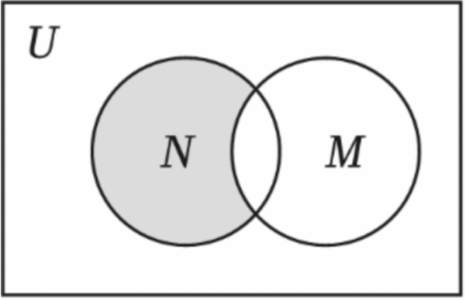
\includegraphics[width=0.30\textwidth]{figures/gao90_q6_venn.png}
\end{center}

\ifanswer
\ans{$N\cap\overline M$}
\fi

\item 已知 $a\in\R$，若关于 $x$ 的方程 $x^2-2x+a-2=0$ 有两个实根 $x_1$、$x_2$，且 $\dfrac1{x_1}+\dfrac1{x_2}=-\dfrac12$，则 $a$ 的值为\blankline[4.4em].

\ifanswer
\solbegin
\step{由于 $x_1$、$x_2$ 是 $x^2-2x+a-2=0$ 的两个实根，}
\step{由韦达定理得 $x_1x_2=a-2$，$x_1+x_2=2$，}
\step{因此 $\dfrac1{x_1}+\dfrac1{x_2}=\dfrac{x_1+x_2}{x_1x_2}=\dfrac2{a-2}=-\dfrac12$，所以 $a-2=-4$，解得 $a=-2$，}
\step{判别式 $\Delta=(-2)^2-4(a-2)=-4a+12$，当 $a=-2$ 时，$\Delta=8+12=20>0$，有两个实根，符合条件，故 $a=-2$.}
\solend
\fi

\item 如果 $-1<x<4$，$-6<y<2$，则 $2x-y$ 的取值范围是\blankline[4.4em].

\ifanswer
\solbegin
\step{因为 $-1<x<4$，$-6<y<2$，所以 $-2<2x<8$，$-2<-y<6$，}
\step{则 $-2+(-2)<2x-y<8+6$，即 $-4<2x-y<14$，}
\step{故 $2x-y$ 的取值范围为 $(-4,14)$.}
\solend
\fi

\item 集合 $A=\left\{x\left|\dfrac6{3-x}\in\Z,x\in\N\right.\right\}$，试用列举法表示集合 $A=\blankline[4.4em]$.

\ifanswer
\solbegin
\step{集合 $A=\left\{x\left|\dfrac6{3-x}\in\Z,x\in\N\right.\right\}$，所以 $3-x$ 可取的值有 $\pm1$、$\pm2$、$\pm3$、$\pm6$，}
\step{又因为 $x\in\N$，所以 $x\in\{0,1,2,4,5,6,9\}$，即 $A=\{0,1,2,4,5,6,9\}$.}
\solend
\fi

\item 不等式 $x^2-ax-b<0$ 的解集是 $(2,3)$，若关于 $x$ 的不等式组 $\begin{cases}(x-a)(3x+b)<0\\ x>t\end{cases}$ 没有实数解，则实数 $t$ 的取值范围是\blankline[4.4em].

\ifanswer
\solbegin
\step{因为等式 $x^2-ax-b<0$ 的解集是 $(2,3)$，所以 $x^2-ax-b=0$ 的根为 $2$、$3$，}
\step{所以 $2+3=a$，$2\times3=-b$，所以 $a=5$，$b=-6$，}
\step{由 $(x-a)(3x+b)=(x-5)(3x-6)<0$ 得 $2<x<5$，}
\step{若关于 $x$ 的不等式组 $\begin{cases}(x-a)(3x+b)<0\\ x>t\end{cases}$ 没有实数解，则 $t\geqslant5$.}
\solend
\fi

\item 若方程 $x^2+2x-m=0$ 有解，则 $m\geqslant a$ 为真命题，则 $a$ 的取值范围为\blankline[4.4em].

\ifanswer
\solbegin
\step{因为方程 $x^2+2x-m=0$ 有解，}
\step{所以 $\Delta=2^2-4\times1\times(-m)=4+4m\geqslant0$，解得 $m\geqslant-1$，}
\step{命题“若方程有解，则 $m\geqslant a$”为真命题，即 $\forall m\in[-1,+\infty)$，$m\geqslant a$ 恒成立，}
\step{因此 $a$ 的取值不能超过集合 $[-1,+\infty)$ 的最小值，即 $a\leqslant-1$，}
\step{综上，$a$ 的取值范围为 $(-\infty,-1]$.}
\solend
\fi

\item 设数集 $M=\left\{x\left|m\leqslant x\leqslant m+\dfrac45\right.\right\}$，$N=\left\{x\left|n-\dfrac14\leqslant x\leqslant n\right.\right\}$，且集合 $M$、$N$ 都是集合 $U=\{x\mid0\leqslant x\leqslant1\}$ 的子集，如果把 $b-a$ 称为非空集合 $\{x\mid a\leqslant x\leqslant b\}$ 的“长度”，那么集合 $M\cap N$ 的“长度”的取值范围为\blankline[4.4em].

\ifanswer
\solbegin
\step{注意到集合 $M$ 的长度为 $\dfrac45$，集合 $N$ 的长度为 $\dfrac14$，均为定值，}
\step{要使得 $M\cap N$ 的“长度”最小，则 $M$ 和 $N$ 尽可能分散到区间的两边，}
\step{长度最小为 $\dfrac45+\dfrac14-1=\dfrac1{20}$；}
\step{要使得 $M\cap N$ 的“长度”最大，则 $M$ 和 $N$ 尽可能集中，}
\step{长度最大就是集合 $N$ 的长度，为 $\dfrac14$，}
\step{故集合 $M\cap N$ 的“长度”的取值范围为 $\left[\dfrac1{20},\dfrac14\right]$.}
\solend
\fi

\end{enumerate}

\bigsec{二、选择题}

\begin{enumerate}
\setcounter{enumi}{12}

\item 设集合 $A=\{x\mid x=2k+1,k\in\Z\}$，$B=\{x\mid x=2k-1,k\in\Z\}$，则 $A$、$B$ 之间的关系是\mbox{（\quad）}

\keepwithprev
A. $B\subsetneq A$\qquad B. $A\subsetneq B$\qquad C. $A=B$\qquad D. 以上都不是

\ifanswer
\solbegin
\step{因为 $k\in\Z$，所以 $2k+1$ 与 $2k-1$ 均表示全体奇数，}
\step{即集合 $A=\{x\mid x=2k+1,k\in\Z\}$ 与 $B=\{x\mid x=2k-1,k\in\Z\}$}
\step{都表示全体奇数构成的集合，所以 $A=B$. 故选 $C$.}
\solend
\fi

\item 已知 $a$、$b\in\R$，且 $a>b$，则下列不等式中一定成立的是\mbox{（\quad）}

\keepwithprev
A. $a+1>b$\qquad B. $a>b+1$\qquad C. $a+1<b+1$\qquad D. $a-1<b-1$

\ifanswer
\solbegin
\step{因为 $a>b$，所以 $a+1>b+1$，$a-1>b-1$，故 $CD$ 错误；}
\step{因为 $a>b$，所以 $a+1>b+0$，即 $a+1>b$ 恒成立，故 $A$ 正确；}
\step{取 $a=1$，$b=0$，$B$ 显然错误.}
\step{故选 $A$.}
\solend
\fi

\item 设 $a$、$b\in\R$，“$a+b>2$ 且 $ab>1$”是“$a>1$，$b>1$”的\mbox{（\quad）}

\keepwithprev
A. 充分不必要条件\qquad B. 必要不充分条件

C. 充要条件\qquad D. 既不充分又不必要条件

\ifanswer
\solbegin
\step{因为 $a>1$ 且 $b>1$，所以 $a+b>2$ 且 $ab>1$，}
\step{若已知 $a+b>2$ 且 $ab>1$，可取 $a=\dfrac12$，$b=8$，也满足已知，}
\step{所以“$a+b>2$ 且 $ab>1$”是“$a>1$ 且 $b>1$”的必要不充分条件，故选 $B$.}
\solend
\fi

\item 设集合 $P_1=\{x\mid x^2+ax+1>0\}$，$P_2=\{x\mid x^2+ax+2>0\}$，$Q_1=\{x\mid x^2+x+b>0\}$，$Q_2=\{x\mid x^2+2x+b>0\}$，其中 $a$、$b\in\R$，下列说法中正确的是\mbox{（\quad）}

\keepwithprev
A. 对任意 $a$，$P_1$ 是 $P_2$ 的子集，对任意 $b$，$Q_1$ 不是 $Q_2$ 的子集

B. 对任意 $a$，$P_1$ 是 $P_2$ 的子集，存在 $b$，使得 $Q_1$ 是 $Q_2$ 的子集

C. 存在 $a$，使得 $P_1$ 不是 $P_2$ 的子集，对任意 $b$，$Q_1$ 不是 $Q_2$ 的子集

D. 存在 $a$，使得 $P_1$ 不是 $P_2$ 的子集，存在 $b$，使得 $Q_1$ 是 $Q_2$ 的子集

\ifanswer
\solbegin
\step{对于集合 $P_1=\{x\mid x^2+ax+1>0\}$，$P_2=\{x\mid x^2+ax+2>0\}$，}
\step{得当 $m\in P_1$ 时，即 $m^2+am+1>0$，得 $m^2+am+2>0$，}
\step{即有 $m\in P_2$，得对任意 $a$，$P_1$ 是 $P_2$ 的子集，}
\step{对于集合 $Q_1=\{x\mid x^2+x+b>0\}$，$Q_2=\{x\mid x^2+2x+b>0\}$，}
\step{当 $b=6$ 时，$Q_1=\{x\mid x^2+x+6>0\}=\R$，$Q_2=\{x\mid x^2+2x+6>0\}=\R$，}
\step{得 $Q_1$ 是 $Q_2$ 的子集，}
\step{当 $b=1$ 时，$Q_1=\{x\mid x^2+x+1>0\}=\R$，}
\step{$Q_2=\{x\mid x^2+2x+1>0\}=\{x\mid x\neq-1\}$，得 $Q_1$ 不是 $Q_2$ 的子集，}
\step{所以存在 $b$，使得 $Q_1$ 是 $Q_2$ 的子集，故选 $B$.}
\solend
\fi

\end{enumerate}

\bigsec{三、解答题}

\begin{enumerate}
\setcounter{enumi}{16}

\item 若 $a$、$b\in\R$，求关于 $x$ 的不等式 $ax\geqslant b$ 的解集.

\ansspace*[9]

\ifanswer
\solbegin
\step{当 $a>0$ 时，原不等式的解集为 $\left\{x\left|x\geqslant\dfrac ba\right.\right\}$；}
\step{当 $a<0$ 时，原不等式的解集为 $\left\{x\left|x\leqslant\dfrac ba\right.\right\}$；}
\step{当 $a=0$，$b\leqslant0$ 时，原不等式的解集为 $\R$；}
\step{当 $a=0$，$b>0$ 时，原不等式的解集为 $\varnothing$.}
\solend
\fi

\item 设集合 $A=\{x\mid x^2+3x+2=0\}$，$B=\{x\mid x^2+(m+1)x+m=0\}$.

（1）用列举法表示集合 $A$；

（2）若 $B\subseteq A$，求实数 $m$ 的值.

\ansspace*[9]

\ifanswer
\solbegin
\stepm{（1）}{集合 $A=\{x\mid x^2+3x+2=0\}$，解方程 $x^2+3x+2=0$，得 $x_1=-2$，$x_2=-1$，}
\step{所以 $A=\{-2,-1\}$.}
\stepm{（2）}{$A=\{-2,-1\}$，$B=\{x\mid x^2+(m+1)x+m=0\}=\{x\mid(x+1)(x+m)=0\}$，}
\step{$B\subseteq A$，所以 $m=1$ 或 $m=2$，所以实数 $m$ 的值为 $1$ 或 $2$.}
\solend
\fi

\item （1）设 $a$、$b$ 是两个正数. 已知 $a>b$，比较 $\dfrac{2a+b}{a+2b}$ 与 $\dfrac ab$ 的值的大小.

（2）用反证法证明：若 $a$、$b\in\R$，且 $x=a^2-2b+1$，$y=b^2-2a+1$，则 $x$、$y$ 中至少有一个不小于 $0$.

\ansspace*[12]

\ifanswer
\solbegin
\stepm{（1）}{$\dfrac{2a+b}{a+2b}-\dfrac ab=\dfrac{b(2a+b)}{b(a+2b)}-\dfrac{a(a+2b)}{b(a+2b)}=\dfrac{b(2a+b)-a(a+2b)}{b(a+2b)}$}
\step{$=\dfrac{2ab+b^2-a^2-2ab}{b(a+2b)}=\dfrac{b^2-a^2}{b(a+2b)}=\dfrac{(b+a)(b-a)}{b(a+2b)}$，}
\step{又 $a>0$，$b>0$，$a>b$，所以 $b+a>0$，$b-a<0$，$b(a+2b)>0$，}
\step{所以 $\dfrac{(b+a)(b-a)}{b(a+2b)}<0$，即 $\dfrac{2a+b}{a+2b}-\dfrac ab<0$，所以 $\dfrac{2a+b}{a+2b}<\dfrac ab$.}
\stepm{（2）}{假设 $x$、$y$ 都小于 $0$，则有 $x+y<0$，}
\step{因为 $x=a^2-2b+1$，$y=b^2-2a+1$，}
\step{所以 $x+y=(a^2-2b+1)+(b^2-2a+1)=(a^2-2a+1)+(b^2-2b+1)$}
\step{$=(a-1)^2+(b-1)^2$，}
\step{又 $a$、$b\in\R$，所以 $(a-1)^2\geqslant0$，$(b-1)^2\geqslant0$，即 $x+y\geqslant0$，}
\step{这与 $x+y<0$ 矛盾，故假设不成立，所以 $x$、$y$ 中至少有一个不小于 $0$.}
\solend
\fi

\item 已知 $m>0$，$p:(x+1)(x-5)\leqslant0$，$q:1-m\leqslant x\leqslant1+m$.

（1）若 $m=5$，$p$、$q$ 有且只有一个为真命题，求实数 $x$ 的取值范围；

（2）若 $p$ 是 $q$ 的充分不必要条件，求实数 $m$ 的取值范围.

\ansspace*[12]

\ifanswer
\solbegin
\stepm{（1）}{对于 $p:(x+1)(x-5)\leqslant0$，解得 $-1\leqslant x\leqslant5$，}
\step{若 $m=5$，则 $q:-4\leqslant x\leqslant6$，}
\step{若 $m=5$，$p$、$q$ 有且只有一个为真命题，则 $p$ 真 $q$ 假或 $p$ 假 $q$ 真，}
\step{若 $p$ 真 $q$ 假，即 $\begin{cases}-1\leqslant x\leqslant5\\ x<-4\ \text{或}\ x>6\end{cases}$，无解，}
\step{若 $p$ 假 $q$ 真，即 $\begin{cases}x<-1\ \text{或}\ x>5\\ -4\leqslant x\leqslant6\end{cases}$，解得 $-4\leqslant x<-1$ 或 $5<x\leqslant6$，}
\step{综上，$-4\leqslant x<-1$ 或 $5<x\leqslant6$，即 $x$ 的取值范围为 $[-4,-1)\cup(5,6]$；}
\stepm{（2）}{若 $p$ 是 $q$ 的充分条件，则有 $\begin{cases}1-m\leqslant-1\\ 5\leqslant1+m\end{cases}$，解得 $m\geqslant4$，}
\step{即 $m$ 的取值范围为 $[4,+\infty)$.}
\solend
\fi

\item 已知关于 $x$ 的不等式：$ax^2-(a+1)x+1<0(a\in\R)$.

（1）当 $a=-2$ 时，求不等式的解集；

（2）当 $a\geqslant0$ 时，求不等式的解集；

（3）命题 $P$：若二次不等式 $ax^2-(a+1)x+1<0$ 的解集为空集，命题 $Q:x^2-2x-a^2+a+1>0$ 对任意实数 $x$ 都成立，若 $P$、$Q$ 中至少有一个真命题，求实数 $a$ 的取值范围.

\ansspace*[14]

\ifanswer
\solbegin
\stepm{（1）}{当 $a=-2$ 时，原不等式为 $2x^2-x-1>0$，即 $(x-1)(2x+1)>0$，}
\step{解得 $x<-\dfrac12$ 或 $x>1$，所以原不等式的解集为 $\left(-\infty,-\dfrac12\right)\cup(1,+\infty)$.}
\stepm{（2）}{当 $a=0$ 时，原不等式为 $-x+1<0$，解得 $x>1$；}
\step{当 $a>0$ 时，原不等式变为 $(ax-1)(x-1)<0$，其对应方程的两根为 $\dfrac1a$，$1$，}
\step{若 $\dfrac1a<1$，即 $a>1$ 时，由 $(ax-1)(x-1)<0$ 解得 $\dfrac1a<x<1$，}
\step{若 $\dfrac1a=1$，即 $a=1$ 时，不等式 $(ax-1)(x-1)<0$ 解集为 $\varnothing$，}
\step{若 $\dfrac1a>1$，即 $0<a<1$ 时，由 $(ax-1)(x-1)<0$ 解得 $1<x<\dfrac1a$，}
\step{综上，当 $a=0$ 时，不等式的解集为 $(1,+\infty)$，}
\step{当 $0<a<1$ 时，不等式的解集为 $\left(1,\dfrac1a\right)$，}
\step{当 $a=1$ 时，不等式的解集为 $\varnothing$，}
\step{当 $a>1$ 时，不等式的解集为 $\left(\dfrac1a,1\right)$.}
\stepm{（3）}{若命题 $P$ 为真命题，}
\step{若 $a<0$，原不等式变为 $(ax-1)(x-1)<0$，其对应方程的两根为 $\dfrac1a$，$1$，}
\step{其解集为 $\left(-\infty,\dfrac1a\right)\cup(1,+\infty)$，不合题意，}
\step{当 $a\geqslant0$ 时，由（2）得当 $a=1$ 时，解集为 $\varnothing$，}
\step{所以命题 $P$ 为真命题，则 $a=1$；}
\step{命题 $Q$ 为真命题，则有相应方程的 $\Delta<0$，即 $a^2-a<0$，解得 $0<a<1$；}
\step{所以当命题 $P$、$Q$ 都为假命题时，$\begin{cases}a\leqslant0\ \text{或}\ a\geqslant1\\ a\neq1\end{cases}$，解得 $a\leqslant0$ 或 $a>1$，}
\step{所以命题 $P$、$Q$ 中至少有一个真命题，则 $0<a\leqslant1$.}
\step{所以实数 $a$ 的取值范围为 $(0,1]$.}
\solend
\fi

\end{enumerate}

\end{document}
"
%
% 原始材料：微信公众号“魔都数学加油站”文章，连载“27学年高一90”；
% 原文标题“27学年高一90——2026-2027年上海市杨思高级中学高一上10月月考”；
% 原文链接：https://mp.weixin.qq.com/s/pvQC5fkWu5Jj3C7dF3-Exw。
% 正文为 8 张 PNG 页（`原图/高一90_杨思高级中学_10月月考/01..08.png`），
% 尺寸混排（第 1、6 页为 2560×3620，其余为 4762×6735），均按页序读取。
%
% 篇幅与题号：原卷自第 3 题起编号（第 1、2 题不在原文内）。填空题 3—12（10 题）、
% 选择题 13—16（4 题）、解答题 17—21（5 题），共 19 题。
%
% 讲评版：第 6 题只印【答案】（“$N\cap\overline M$”），本稿只给 \ans{}；
% 其余 18 题印【解析】，其中选择题答案在解析末句“故选 C／A／B／B”。
% 第 6 题题干带一幅韦恩图（全集 $U$、集合 $M$、$N$ 与阴影部分），三版都出。
%
% 副标题：原卷未印副标题。本稿按内容标作“集合与常用逻辑用语、不等式”。
%
% 原卷笔误/存疑（均照录未改，正文对应处另有 % 注）：
%   ① 第 6 题的韦恩图阴影为 $N$ 中不属于 $M$ 的部分，与所印答案 $N\cap\overline M$ 一致；
%      图与答案均照录。原卷把“（请用各集合的交，并，补表示）”的逗号排作全角逗号，照录；
%   ② 第 12 题题干“如果把 $b-a$ 称为非空集合 $\{x\mid a\leqslant x\leqslant b\}$ 的‘长度’”
%      与本稿统一后的 $\R$、$\Z$、$\N$ 记号无关，原文用斜体 $R$、$Z$、$N$，按惯例改写。
%
% 与原卷的排版差异：
%   ① 原卷每题下直接印【答案】/【解析】，本稿按全稿惯例将答案与解析置于答案版；
%   ② 原卷未印副标题，本稿补出；填空横线统一排 \blankline[4.4em]；
%   ③ 原卷数集记号排斜体 $R$、$Z$、$N$，本稿按全稿惯例改用 $\R$、$\Z$、$\N$；
%   ④ 第 17—21 题的子问用行内“（1）（2）（3）”段，解析中的子问标号用 \stepm；
%   ⑤ 解答题按惯例加 \ansspace；选择题括号排 \mbox{（\quad）}；
%   ⑥ 第 6 题的韦恩图原卷排在题干右侧、文字绕排，本稿改排为题干后的居中图
%      （自原图裁切、去粉色水印后转灰度）。
%
% 行数核对：逐题数 \step/\stepm 条数，合计 94 条（Q3：2；Q4：2；Q5：1；Q6：0；
% Q7：4；Q8：3；Q9：2；Q10：4；Q11：5；Q12：6；Q13：3；Q14：4；Q15：3；Q16：9；
% Q17：4；Q18：4；Q19：10；Q20：8；Q21：20）。第 6 题只印【答案】，不计入 \step 账。
% 原卷解析的换行按语意合并，未逐行强拆。
%
\documentclass[a4paper,11pt]{article}
\usepackage{common}

\begin{document}

\examtitlest[7]{2026--2027 年杨思高级中学高一上 10 月月考}{集合与常用逻辑用语、不等式}

\bigsec{一、填空题}

\begin{enumerate}
\setcounter{enumi}{2}

\item 已知集合 $A=\{x\mid6x+a>0\}$，若 $1\notin A$，则实数 $a$ 的取值范围是\blankline[4.4em].

\ifanswer
\solbegin
\step{集合 $A=\{x\mid6x+a>0\}$，若 $1\notin A$，则 $6+a\leqslant0$ 恒成立，故 $a\leqslant-6$，}
\step{故实数 $a$ 的取值范围是 $(-\infty,-6]$.}
\solend
\fi

\item 设全集 $U=\R$，集合 $A=\{x\mid-1\leqslant x\leqslant1\}$，$B=\{x\mid0<x<2\}$，则 $\overline{A\cup B}=\blankline[4.4em]$.

\ifanswer
\solbegin
\step{$B=\{x\mid0<x<2\}$，$A=\{x\mid-1\leqslant x\leqslant1\}$，所以 $A\cup B=\{x\mid-1\leqslant x<2\}$，}
\step{又因为全集 $U=\R$，所以 $\overline{A\cup B}=(-\infty,-1)\cup[2,+\infty)$.}
\solend
\fi

\item 集合 $A=\{(x,y)\mid y=-x\}$，$B=\{(x,y)\mid y=2x-4\}$，则 $A\cap B=\blankline[4.4em]$.

\ifanswer
\solbegin
\step{联立 $\begin{cases}y=-x\\ y=2x-4\end{cases}$，解得 $\begin{cases}x=\dfrac43\\[0.2em] y=-\dfrac43\end{cases}$，即 $A\cap B=\left\{\left(\dfrac43,-\dfrac43\right)\right\}$.}
\solend
\fi

\item 设 $U$ 是全集，$M$、$N$ 是 $U$ 的子集，则图中阴影部分所表示的集合是\blankline[4.4em].

（请用各集合的交，并，补表示）

\begin{center}
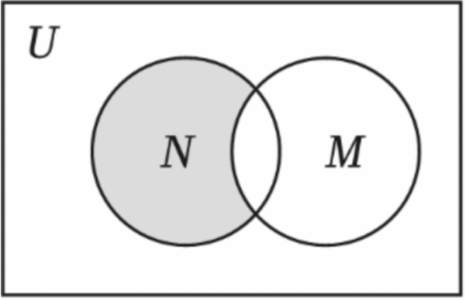
\includegraphics[width=0.30\textwidth]{figures/gao90_q6_venn.png}
\end{center}

\ifanswer
\ans{$N\cap\overline M$}
\fi

\item 已知 $a\in\R$，若关于 $x$ 的方程 $x^2-2x+a-2=0$ 有两个实根 $x_1$、$x_2$，且 $\dfrac1{x_1}+\dfrac1{x_2}=-\dfrac12$，则 $a$ 的值为\blankline[4.4em].

\ifanswer
\solbegin
\step{由于 $x_1$、$x_2$ 是 $x^2-2x+a-2=0$ 的两个实根，}
\step{由韦达定理得 $x_1x_2=a-2$，$x_1+x_2=2$，}
\step{因此 $\dfrac1{x_1}+\dfrac1{x_2}=\dfrac{x_1+x_2}{x_1x_2}=\dfrac2{a-2}=-\dfrac12$，所以 $a-2=-4$，解得 $a=-2$，}
\step{判别式 $\Delta=(-2)^2-4(a-2)=-4a+12$，当 $a=-2$ 时，$\Delta=8+12=20>0$，有两个实根，符合条件，故 $a=-2$.}
\solend
\fi

\item 如果 $-1<x<4$，$-6<y<2$，则 $2x-y$ 的取值范围是\blankline[4.4em].

\ifanswer
\solbegin
\step{因为 $-1<x<4$，$-6<y<2$，所以 $-2<2x<8$，$-2<-y<6$，}
\step{则 $-2+(-2)<2x-y<8+6$，即 $-4<2x-y<14$，}
\step{故 $2x-y$ 的取值范围为 $(-4,14)$.}
\solend
\fi

\item 集合 $A=\left\{x\left|\dfrac6{3-x}\in\Z,x\in\N\right.\right\}$，试用列举法表示集合 $A=\blankline[4.4em]$.

\ifanswer
\solbegin
\step{集合 $A=\left\{x\left|\dfrac6{3-x}\in\Z,x\in\N\right.\right\}$，所以 $3-x$ 可取的值有 $\pm1$、$\pm2$、$\pm3$、$\pm6$，}
\step{又因为 $x\in\N$，所以 $x\in\{0,1,2,4,5,6,9\}$，即 $A=\{0,1,2,4,5,6,9\}$.}
\solend
\fi

\item 不等式 $x^2-ax-b<0$ 的解集是 $(2,3)$，若关于 $x$ 的不等式组 $\begin{cases}(x-a)(3x+b)<0\\ x>t\end{cases}$ 没有实数解，则实数 $t$ 的取值范围是\blankline[4.4em].

\ifanswer
\solbegin
\step{因为等式 $x^2-ax-b<0$ 的解集是 $(2,3)$，所以 $x^2-ax-b=0$ 的根为 $2$、$3$，}
\step{所以 $2+3=a$，$2\times3=-b$，所以 $a=5$，$b=-6$，}
\step{由 $(x-a)(3x+b)=(x-5)(3x-6)<0$ 得 $2<x<5$，}
\step{若关于 $x$ 的不等式组 $\begin{cases}(x-a)(3x+b)<0\\ x>t\end{cases}$ 没有实数解，则 $t\geqslant5$.}
\solend
\fi

\item 若方程 $x^2+2x-m=0$ 有解，则 $m\geqslant a$ 为真命题，则 $a$ 的取值范围为\blankline[4.4em].

\ifanswer
\solbegin
\step{因为方程 $x^2+2x-m=0$ 有解，}
\step{所以 $\Delta=2^2-4\times1\times(-m)=4+4m\geqslant0$，解得 $m\geqslant-1$，}
\step{命题“若方程有解，则 $m\geqslant a$”为真命题，即 $\forall m\in[-1,+\infty)$，$m\geqslant a$ 恒成立，}
\step{因此 $a$ 的取值不能超过集合 $[-1,+\infty)$ 的最小值，即 $a\leqslant-1$，}
\step{综上，$a$ 的取值范围为 $(-\infty,-1]$.}
\solend
\fi

\item 设数集 $M=\left\{x\left|m\leqslant x\leqslant m+\dfrac45\right.\right\}$，$N=\left\{x\left|n-\dfrac14\leqslant x\leqslant n\right.\right\}$，且集合 $M$、$N$ 都是集合 $U=\{x\mid0\leqslant x\leqslant1\}$ 的子集，如果把 $b-a$ 称为非空集合 $\{x\mid a\leqslant x\leqslant b\}$ 的“长度”，那么集合 $M\cap N$ 的“长度”的取值范围为\blankline[4.4em].

\ifanswer
\solbegin
\step{注意到集合 $M$ 的长度为 $\dfrac45$，集合 $N$ 的长度为 $\dfrac14$，均为定值，}
\step{要使得 $M\cap N$ 的“长度”最小，则 $M$ 和 $N$ 尽可能分散到区间的两边，}
\step{长度最小为 $\dfrac45+\dfrac14-1=\dfrac1{20}$；}
\step{要使得 $M\cap N$ 的“长度”最大，则 $M$ 和 $N$ 尽可能集中，}
\step{长度最大就是集合 $N$ 的长度，为 $\dfrac14$，}
\step{故集合 $M\cap N$ 的“长度”的取值范围为 $\left[\dfrac1{20},\dfrac14\right]$.}
\solend
\fi

\end{enumerate}

\bigsec{二、选择题}

\begin{enumerate}
\setcounter{enumi}{12}

\item 设集合 $A=\{x\mid x=2k+1,k\in\Z\}$，$B=\{x\mid x=2k-1,k\in\Z\}$，则 $A$、$B$ 之间的关系是\mbox{（\quad）}

\keepwithprev
A. $B\subsetneq A$\qquad B. $A\subsetneq B$\qquad C. $A=B$\qquad D. 以上都不是

\ifanswer
\solbegin
\step{因为 $k\in\Z$，所以 $2k+1$ 与 $2k-1$ 均表示全体奇数，}
\step{即集合 $A=\{x\mid x=2k+1,k\in\Z\}$ 与 $B=\{x\mid x=2k-1,k\in\Z\}$}
\step{都表示全体奇数构成的集合，所以 $A=B$. 故选 $C$.}
\solend
\fi

\item 已知 $a$、$b\in\R$，且 $a>b$，则下列不等式中一定成立的是\mbox{（\quad）}

\keepwithprev
A. $a+1>b$\qquad B. $a>b+1$\qquad C. $a+1<b+1$\qquad D. $a-1<b-1$

\ifanswer
\solbegin
\step{因为 $a>b$，所以 $a+1>b+1$，$a-1>b-1$，故 $CD$ 错误；}
\step{因为 $a>b$，所以 $a+1>b+0$，即 $a+1>b$ 恒成立，故 $A$ 正确；}
\step{取 $a=1$，$b=0$，$B$ 显然错误.}
\step{故选 $A$.}
\solend
\fi

\item 设 $a$、$b\in\R$，“$a+b>2$ 且 $ab>1$”是“$a>1$，$b>1$”的\mbox{（\quad）}

\keepwithprev
A. 充分不必要条件\qquad B. 必要不充分条件

C. 充要条件\qquad D. 既不充分又不必要条件

\ifanswer
\solbegin
\step{因为 $a>1$ 且 $b>1$，所以 $a+b>2$ 且 $ab>1$，}
\step{若已知 $a+b>2$ 且 $ab>1$，可取 $a=\dfrac12$，$b=8$，也满足已知，}
\step{所以“$a+b>2$ 且 $ab>1$”是“$a>1$ 且 $b>1$”的必要不充分条件，故选 $B$.}
\solend
\fi

\item 设集合 $P_1=\{x\mid x^2+ax+1>0\}$，$P_2=\{x\mid x^2+ax+2>0\}$，$Q_1=\{x\mid x^2+x+b>0\}$，$Q_2=\{x\mid x^2+2x+b>0\}$，其中 $a$、$b\in\R$，下列说法中正确的是\mbox{（\quad）}

\keepwithprev
A. 对任意 $a$，$P_1$ 是 $P_2$ 的子集，对任意 $b$，$Q_1$ 不是 $Q_2$ 的子集

B. 对任意 $a$，$P_1$ 是 $P_2$ 的子集，存在 $b$，使得 $Q_1$ 是 $Q_2$ 的子集

C. 存在 $a$，使得 $P_1$ 不是 $P_2$ 的子集，对任意 $b$，$Q_1$ 不是 $Q_2$ 的子集

D. 存在 $a$，使得 $P_1$ 不是 $P_2$ 的子集，存在 $b$，使得 $Q_1$ 是 $Q_2$ 的子集

\ifanswer
\solbegin
\step{对于集合 $P_1=\{x\mid x^2+ax+1>0\}$，$P_2=\{x\mid x^2+ax+2>0\}$，}
\step{得当 $m\in P_1$ 时，即 $m^2+am+1>0$，得 $m^2+am+2>0$，}
\step{即有 $m\in P_2$，得对任意 $a$，$P_1$ 是 $P_2$ 的子集，}
\step{对于集合 $Q_1=\{x\mid x^2+x+b>0\}$，$Q_2=\{x\mid x^2+2x+b>0\}$，}
\step{当 $b=6$ 时，$Q_1=\{x\mid x^2+x+6>0\}=\R$，$Q_2=\{x\mid x^2+2x+6>0\}=\R$，}
\step{得 $Q_1$ 是 $Q_2$ 的子集，}
\step{当 $b=1$ 时，$Q_1=\{x\mid x^2+x+1>0\}=\R$，}
\step{$Q_2=\{x\mid x^2+2x+1>0\}=\{x\mid x\neq-1\}$，得 $Q_1$ 不是 $Q_2$ 的子集，}
\step{所以存在 $b$，使得 $Q_1$ 是 $Q_2$ 的子集，故选 $B$.}
\solend
\fi

\end{enumerate}

\bigsec{三、解答题}

\begin{enumerate}
\setcounter{enumi}{16}

\item 若 $a$、$b\in\R$，求关于 $x$ 的不等式 $ax\geqslant b$ 的解集.

\ansspace*[9]

\ifanswer
\solbegin
\step{当 $a>0$ 时，原不等式的解集为 $\left\{x\left|x\geqslant\dfrac ba\right.\right\}$；}
\step{当 $a<0$ 时，原不等式的解集为 $\left\{x\left|x\leqslant\dfrac ba\right.\right\}$；}
\step{当 $a=0$，$b\leqslant0$ 时，原不等式的解集为 $\R$；}
\step{当 $a=0$，$b>0$ 时，原不等式的解集为 $\varnothing$.}
\solend
\fi

\item 设集合 $A=\{x\mid x^2+3x+2=0\}$，$B=\{x\mid x^2+(m+1)x+m=0\}$.

（1）用列举法表示集合 $A$；

（2）若 $B\subseteq A$，求实数 $m$ 的值.

\ansspace*[9]

\ifanswer
\solbegin
\stepm{（1）}{集合 $A=\{x\mid x^2+3x+2=0\}$，解方程 $x^2+3x+2=0$，得 $x_1=-2$，$x_2=-1$，}
\step{所以 $A=\{-2,-1\}$.}
\stepm{（2）}{$A=\{-2,-1\}$，$B=\{x\mid x^2+(m+1)x+m=0\}=\{x\mid(x+1)(x+m)=0\}$，}
\step{$B\subseteq A$，所以 $m=1$ 或 $m=2$，所以实数 $m$ 的值为 $1$ 或 $2$.}
\solend
\fi

\item （1）设 $a$、$b$ 是两个正数. 已知 $a>b$，比较 $\dfrac{2a+b}{a+2b}$ 与 $\dfrac ab$ 的值的大小.

（2）用反证法证明：若 $a$、$b\in\R$，且 $x=a^2-2b+1$，$y=b^2-2a+1$，则 $x$、$y$ 中至少有一个不小于 $0$.

\ansspace*[12]

\ifanswer
\solbegin
\stepm{（1）}{$\dfrac{2a+b}{a+2b}-\dfrac ab=\dfrac{b(2a+b)}{b(a+2b)}-\dfrac{a(a+2b)}{b(a+2b)}=\dfrac{b(2a+b)-a(a+2b)}{b(a+2b)}$}
\step{$=\dfrac{2ab+b^2-a^2-2ab}{b(a+2b)}=\dfrac{b^2-a^2}{b(a+2b)}=\dfrac{(b+a)(b-a)}{b(a+2b)}$，}
\step{又 $a>0$，$b>0$，$a>b$，所以 $b+a>0$，$b-a<0$，$b(a+2b)>0$，}
\step{所以 $\dfrac{(b+a)(b-a)}{b(a+2b)}<0$，即 $\dfrac{2a+b}{a+2b}-\dfrac ab<0$，所以 $\dfrac{2a+b}{a+2b}<\dfrac ab$.}
\stepm{（2）}{假设 $x$、$y$ 都小于 $0$，则有 $x+y<0$，}
\step{因为 $x=a^2-2b+1$，$y=b^2-2a+1$，}
\step{所以 $x+y=(a^2-2b+1)+(b^2-2a+1)=(a^2-2a+1)+(b^2-2b+1)$}
\step{$=(a-1)^2+(b-1)^2$，}
\step{又 $a$、$b\in\R$，所以 $(a-1)^2\geqslant0$，$(b-1)^2\geqslant0$，即 $x+y\geqslant0$，}
\step{这与 $x+y<0$ 矛盾，故假设不成立，所以 $x$、$y$ 中至少有一个不小于 $0$.}
\solend
\fi

\item 已知 $m>0$，$p:(x+1)(x-5)\leqslant0$，$q:1-m\leqslant x\leqslant1+m$.

（1）若 $m=5$，$p$、$q$ 有且只有一个为真命题，求实数 $x$ 的取值范围；

（2）若 $p$ 是 $q$ 的充分不必要条件，求实数 $m$ 的取值范围.

\ansspace*[12]

\ifanswer
\solbegin
\stepm{（1）}{对于 $p:(x+1)(x-5)\leqslant0$，解得 $-1\leqslant x\leqslant5$，}
\step{若 $m=5$，则 $q:-4\leqslant x\leqslant6$，}
\step{若 $m=5$，$p$、$q$ 有且只有一个为真命题，则 $p$ 真 $q$ 假或 $p$ 假 $q$ 真，}
\step{若 $p$ 真 $q$ 假，即 $\begin{cases}-1\leqslant x\leqslant5\\ x<-4\ \text{或}\ x>6\end{cases}$，无解，}
\step{若 $p$ 假 $q$ 真，即 $\begin{cases}x<-1\ \text{或}\ x>5\\ -4\leqslant x\leqslant6\end{cases}$，解得 $-4\leqslant x<-1$ 或 $5<x\leqslant6$，}
\step{综上，$-4\leqslant x<-1$ 或 $5<x\leqslant6$，即 $x$ 的取值范围为 $[-4,-1)\cup(5,6]$；}
\stepm{（2）}{若 $p$ 是 $q$ 的充分条件，则有 $\begin{cases}1-m\leqslant-1\\ 5\leqslant1+m\end{cases}$，解得 $m\geqslant4$，}
\step{即 $m$ 的取值范围为 $[4,+\infty)$.}
\solend
\fi

\item 已知关于 $x$ 的不等式：$ax^2-(a+1)x+1<0(a\in\R)$.

（1）当 $a=-2$ 时，求不等式的解集；

（2）当 $a\geqslant0$ 时，求不等式的解集；

（3）命题 $P$：若二次不等式 $ax^2-(a+1)x+1<0$ 的解集为空集，命题 $Q:x^2-2x-a^2+a+1>0$ 对任意实数 $x$ 都成立，若 $P$、$Q$ 中至少有一个真命题，求实数 $a$ 的取值范围.

\ansspace*[14]

\ifanswer
\solbegin
\stepm{（1）}{当 $a=-2$ 时，原不等式为 $2x^2-x-1>0$，即 $(x-1)(2x+1)>0$，}
\step{解得 $x<-\dfrac12$ 或 $x>1$，所以原不等式的解集为 $\left(-\infty,-\dfrac12\right)\cup(1,+\infty)$.}
\stepm{（2）}{当 $a=0$ 时，原不等式为 $-x+1<0$，解得 $x>1$；}
\step{当 $a>0$ 时，原不等式变为 $(ax-1)(x-1)<0$，其对应方程的两根为 $\dfrac1a$，$1$，}
\step{若 $\dfrac1a<1$，即 $a>1$ 时，由 $(ax-1)(x-1)<0$ 解得 $\dfrac1a<x<1$，}
\step{若 $\dfrac1a=1$，即 $a=1$ 时，不等式 $(ax-1)(x-1)<0$ 解集为 $\varnothing$，}
\step{若 $\dfrac1a>1$，即 $0<a<1$ 时，由 $(ax-1)(x-1)<0$ 解得 $1<x<\dfrac1a$，}
\step{综上，当 $a=0$ 时，不等式的解集为 $(1,+\infty)$，}
\step{当 $0<a<1$ 时，不等式的解集为 $\left(1,\dfrac1a\right)$，}
\step{当 $a=1$ 时，不等式的解集为 $\varnothing$，}
\step{当 $a>1$ 时，不等式的解集为 $\left(\dfrac1a,1\right)$.}
\stepm{（3）}{若命题 $P$ 为真命题，}
\step{若 $a<0$，原不等式变为 $(ax-1)(x-1)<0$，其对应方程的两根为 $\dfrac1a$，$1$，}
\step{其解集为 $\left(-\infty,\dfrac1a\right)\cup(1,+\infty)$，不合题意，}
\step{当 $a\geqslant0$ 时，由（2）得当 $a=1$ 时，解集为 $\varnothing$，}
\step{所以命题 $P$ 为真命题，则 $a=1$；}
\step{命题 $Q$ 为真命题，则有相应方程的 $\Delta<0$，即 $a^2-a<0$，解得 $0<a<1$；}
\step{所以当命题 $P$、$Q$ 都为假命题时，$\begin{cases}a\leqslant0\ \text{或}\ a\geqslant1\\ a\neq1\end{cases}$，解得 $a\leqslant0$ 或 $a>1$，}
\step{所以命题 $P$、$Q$ 中至少有一个真命题，则 $0<a\leqslant1$.}
\step{所以实数 $a$ 的取值范围为 $(0,1]$.}
\solend
\fi

\end{enumerate}

\end{document}
"
% 紧凑版：xelatex "\def\iscompact{1}% 高一90_杨思高级中学_10月月考.tex
%   —— 高一上数学“2026-2027 年杨思高级中学高一上 10 月月考”（讲评版）
% 试卷版：xelatex 高一90_杨思高级中学_10月月考.tex
% 答案版：xelatex "\def\isanswer{1}% 高一90_杨思高级中学_10月月考.tex
%   —— 高一上数学“2026-2027 年杨思高级中学高一上 10 月月考”（讲评版）
% 试卷版：xelatex 高一90_杨思高级中学_10月月考.tex
% 答案版：xelatex "\def\isanswer{1}\input{高一90_杨思高级中学_10月月考.tex}"
% 紧凑版：xelatex "\def\iscompact{1}\input{高一90_杨思高级中学_10月月考.tex}"
%
% 原始材料：微信公众号“魔都数学加油站”文章，连载“27学年高一90”；
% 原文标题“27学年高一90——2026-2027年上海市杨思高级中学高一上10月月考”；
% 原文链接：https://mp.weixin.qq.com/s/pvQC5fkWu5Jj3C7dF3-Exw。
% 正文为 8 张 PNG 页（`原图/高一90_杨思高级中学_10月月考/01..08.png`），
% 尺寸混排（第 1、6 页为 2560×3620，其余为 4762×6735），均按页序读取。
%
% 篇幅与题号：原卷自第 3 题起编号（第 1、2 题不在原文内）。填空题 3—12（10 题）、
% 选择题 13—16（4 题）、解答题 17—21（5 题），共 19 题。
%
% 讲评版：第 6 题只印【答案】（“$N\cap\overline M$”），本稿只给 \ans{}；
% 其余 18 题印【解析】，其中选择题答案在解析末句“故选 C／A／B／B”。
% 第 6 题题干带一幅韦恩图（全集 $U$、集合 $M$、$N$ 与阴影部分），三版都出。
%
% 副标题：原卷未印副标题。本稿按内容标作“集合与常用逻辑用语、不等式”。
%
% 原卷笔误/存疑（均照录未改，正文对应处另有 % 注）：
%   ① 第 6 题的韦恩图阴影为 $N$ 中不属于 $M$ 的部分，与所印答案 $N\cap\overline M$ 一致；
%      图与答案均照录。原卷把“（请用各集合的交，并，补表示）”的逗号排作全角逗号，照录；
%   ② 第 12 题题干“如果把 $b-a$ 称为非空集合 $\{x\mid a\leqslant x\leqslant b\}$ 的‘长度’”
%      与本稿统一后的 $\R$、$\Z$、$\N$ 记号无关，原文用斜体 $R$、$Z$、$N$，按惯例改写。
%
% 与原卷的排版差异：
%   ① 原卷每题下直接印【答案】/【解析】，本稿按全稿惯例将答案与解析置于答案版；
%   ② 原卷未印副标题，本稿补出；填空横线统一排 \blankline[4.4em]；
%   ③ 原卷数集记号排斜体 $R$、$Z$、$N$，本稿按全稿惯例改用 $\R$、$\Z$、$\N$；
%   ④ 第 17—21 题的子问用行内“（1）（2）（3）”段，解析中的子问标号用 \stepm；
%   ⑤ 解答题按惯例加 \ansspace；选择题括号排 \mbox{（\quad）}；
%   ⑥ 第 6 题的韦恩图原卷排在题干右侧、文字绕排，本稿改排为题干后的居中图
%      （自原图裁切、去粉色水印后转灰度）。
%
% 行数核对：逐题数 \step/\stepm 条数，合计 94 条（Q3：2；Q4：2；Q5：1；Q6：0；
% Q7：4；Q8：3；Q9：2；Q10：4；Q11：5；Q12：6；Q13：3；Q14：4；Q15：3；Q16：9；
% Q17：4；Q18：4；Q19：10；Q20：8；Q21：20）。第 6 题只印【答案】，不计入 \step 账。
% 原卷解析的换行按语意合并，未逐行强拆。
%
\documentclass[a4paper,11pt]{article}
\usepackage{common}

\begin{document}

\examtitlest[7]{2026--2027 年杨思高级中学高一上 10 月月考}{集合与常用逻辑用语、不等式}

\bigsec{一、填空题}

\begin{enumerate}
\setcounter{enumi}{2}

\item 已知集合 $A=\{x\mid6x+a>0\}$，若 $1\notin A$，则实数 $a$ 的取值范围是\blankline[4.4em].

\ifanswer
\solbegin
\step{集合 $A=\{x\mid6x+a>0\}$，若 $1\notin A$，则 $6+a\leqslant0$ 恒成立，故 $a\leqslant-6$，}
\step{故实数 $a$ 的取值范围是 $(-\infty,-6]$.}
\solend
\fi

\item 设全集 $U=\R$，集合 $A=\{x\mid-1\leqslant x\leqslant1\}$，$B=\{x\mid0<x<2\}$，则 $\overline{A\cup B}=\blankline[4.4em]$.

\ifanswer
\solbegin
\step{$B=\{x\mid0<x<2\}$，$A=\{x\mid-1\leqslant x\leqslant1\}$，所以 $A\cup B=\{x\mid-1\leqslant x<2\}$，}
\step{又因为全集 $U=\R$，所以 $\overline{A\cup B}=(-\infty,-1)\cup[2,+\infty)$.}
\solend
\fi

\item 集合 $A=\{(x,y)\mid y=-x\}$，$B=\{(x,y)\mid y=2x-4\}$，则 $A\cap B=\blankline[4.4em]$.

\ifanswer
\solbegin
\step{联立 $\begin{cases}y=-x\\ y=2x-4\end{cases}$，解得 $\begin{cases}x=\dfrac43\\[0.2em] y=-\dfrac43\end{cases}$，即 $A\cap B=\left\{\left(\dfrac43,-\dfrac43\right)\right\}$.}
\solend
\fi

\item 设 $U$ 是全集，$M$、$N$ 是 $U$ 的子集，则图中阴影部分所表示的集合是\blankline[4.4em].

（请用各集合的交，并，补表示）

\begin{center}
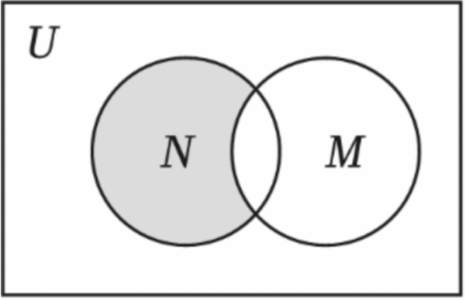
\includegraphics[width=0.30\textwidth]{figures/gao90_q6_venn.png}
\end{center}

\ifanswer
\ans{$N\cap\overline M$}
\fi

\item 已知 $a\in\R$，若关于 $x$ 的方程 $x^2-2x+a-2=0$ 有两个实根 $x_1$、$x_2$，且 $\dfrac1{x_1}+\dfrac1{x_2}=-\dfrac12$，则 $a$ 的值为\blankline[4.4em].

\ifanswer
\solbegin
\step{由于 $x_1$、$x_2$ 是 $x^2-2x+a-2=0$ 的两个实根，}
\step{由韦达定理得 $x_1x_2=a-2$，$x_1+x_2=2$，}
\step{因此 $\dfrac1{x_1}+\dfrac1{x_2}=\dfrac{x_1+x_2}{x_1x_2}=\dfrac2{a-2}=-\dfrac12$，所以 $a-2=-4$，解得 $a=-2$，}
\step{判别式 $\Delta=(-2)^2-4(a-2)=-4a+12$，当 $a=-2$ 时，$\Delta=8+12=20>0$，有两个实根，符合条件，故 $a=-2$.}
\solend
\fi

\item 如果 $-1<x<4$，$-6<y<2$，则 $2x-y$ 的取值范围是\blankline[4.4em].

\ifanswer
\solbegin
\step{因为 $-1<x<4$，$-6<y<2$，所以 $-2<2x<8$，$-2<-y<6$，}
\step{则 $-2+(-2)<2x-y<8+6$，即 $-4<2x-y<14$，}
\step{故 $2x-y$ 的取值范围为 $(-4,14)$.}
\solend
\fi

\item 集合 $A=\left\{x\left|\dfrac6{3-x}\in\Z,x\in\N\right.\right\}$，试用列举法表示集合 $A=\blankline[4.4em]$.

\ifanswer
\solbegin
\step{集合 $A=\left\{x\left|\dfrac6{3-x}\in\Z,x\in\N\right.\right\}$，所以 $3-x$ 可取的值有 $\pm1$、$\pm2$、$\pm3$、$\pm6$，}
\step{又因为 $x\in\N$，所以 $x\in\{0,1,2,4,5,6,9\}$，即 $A=\{0,1,2,4,5,6,9\}$.}
\solend
\fi

\item 不等式 $x^2-ax-b<0$ 的解集是 $(2,3)$，若关于 $x$ 的不等式组 $\begin{cases}(x-a)(3x+b)<0\\ x>t\end{cases}$ 没有实数解，则实数 $t$ 的取值范围是\blankline[4.4em].

\ifanswer
\solbegin
\step{因为等式 $x^2-ax-b<0$ 的解集是 $(2,3)$，所以 $x^2-ax-b=0$ 的根为 $2$、$3$，}
\step{所以 $2+3=a$，$2\times3=-b$，所以 $a=5$，$b=-6$，}
\step{由 $(x-a)(3x+b)=(x-5)(3x-6)<0$ 得 $2<x<5$，}
\step{若关于 $x$ 的不等式组 $\begin{cases}(x-a)(3x+b)<0\\ x>t\end{cases}$ 没有实数解，则 $t\geqslant5$.}
\solend
\fi

\item 若方程 $x^2+2x-m=0$ 有解，则 $m\geqslant a$ 为真命题，则 $a$ 的取值范围为\blankline[4.4em].

\ifanswer
\solbegin
\step{因为方程 $x^2+2x-m=0$ 有解，}
\step{所以 $\Delta=2^2-4\times1\times(-m)=4+4m\geqslant0$，解得 $m\geqslant-1$，}
\step{命题“若方程有解，则 $m\geqslant a$”为真命题，即 $\forall m\in[-1,+\infty)$，$m\geqslant a$ 恒成立，}
\step{因此 $a$ 的取值不能超过集合 $[-1,+\infty)$ 的最小值，即 $a\leqslant-1$，}
\step{综上，$a$ 的取值范围为 $(-\infty,-1]$.}
\solend
\fi

\item 设数集 $M=\left\{x\left|m\leqslant x\leqslant m+\dfrac45\right.\right\}$，$N=\left\{x\left|n-\dfrac14\leqslant x\leqslant n\right.\right\}$，且集合 $M$、$N$ 都是集合 $U=\{x\mid0\leqslant x\leqslant1\}$ 的子集，如果把 $b-a$ 称为非空集合 $\{x\mid a\leqslant x\leqslant b\}$ 的“长度”，那么集合 $M\cap N$ 的“长度”的取值范围为\blankline[4.4em].

\ifanswer
\solbegin
\step{注意到集合 $M$ 的长度为 $\dfrac45$，集合 $N$ 的长度为 $\dfrac14$，均为定值，}
\step{要使得 $M\cap N$ 的“长度”最小，则 $M$ 和 $N$ 尽可能分散到区间的两边，}
\step{长度最小为 $\dfrac45+\dfrac14-1=\dfrac1{20}$；}
\step{要使得 $M\cap N$ 的“长度”最大，则 $M$ 和 $N$ 尽可能集中，}
\step{长度最大就是集合 $N$ 的长度，为 $\dfrac14$，}
\step{故集合 $M\cap N$ 的“长度”的取值范围为 $\left[\dfrac1{20},\dfrac14\right]$.}
\solend
\fi

\end{enumerate}

\bigsec{二、选择题}

\begin{enumerate}
\setcounter{enumi}{12}

\item 设集合 $A=\{x\mid x=2k+1,k\in\Z\}$，$B=\{x\mid x=2k-1,k\in\Z\}$，则 $A$、$B$ 之间的关系是\mbox{（\quad）}

\keepwithprev
A. $B\subsetneq A$\qquad B. $A\subsetneq B$\qquad C. $A=B$\qquad D. 以上都不是

\ifanswer
\solbegin
\step{因为 $k\in\Z$，所以 $2k+1$ 与 $2k-1$ 均表示全体奇数，}
\step{即集合 $A=\{x\mid x=2k+1,k\in\Z\}$ 与 $B=\{x\mid x=2k-1,k\in\Z\}$}
\step{都表示全体奇数构成的集合，所以 $A=B$. 故选 $C$.}
\solend
\fi

\item 已知 $a$、$b\in\R$，且 $a>b$，则下列不等式中一定成立的是\mbox{（\quad）}

\keepwithprev
A. $a+1>b$\qquad B. $a>b+1$\qquad C. $a+1<b+1$\qquad D. $a-1<b-1$

\ifanswer
\solbegin
\step{因为 $a>b$，所以 $a+1>b+1$，$a-1>b-1$，故 $CD$ 错误；}
\step{因为 $a>b$，所以 $a+1>b+0$，即 $a+1>b$ 恒成立，故 $A$ 正确；}
\step{取 $a=1$，$b=0$，$B$ 显然错误.}
\step{故选 $A$.}
\solend
\fi

\item 设 $a$、$b\in\R$，“$a+b>2$ 且 $ab>1$”是“$a>1$，$b>1$”的\mbox{（\quad）}

\keepwithprev
A. 充分不必要条件\qquad B. 必要不充分条件

C. 充要条件\qquad D. 既不充分又不必要条件

\ifanswer
\solbegin
\step{因为 $a>1$ 且 $b>1$，所以 $a+b>2$ 且 $ab>1$，}
\step{若已知 $a+b>2$ 且 $ab>1$，可取 $a=\dfrac12$，$b=8$，也满足已知，}
\step{所以“$a+b>2$ 且 $ab>1$”是“$a>1$ 且 $b>1$”的必要不充分条件，故选 $B$.}
\solend
\fi

\item 设集合 $P_1=\{x\mid x^2+ax+1>0\}$，$P_2=\{x\mid x^2+ax+2>0\}$，$Q_1=\{x\mid x^2+x+b>0\}$，$Q_2=\{x\mid x^2+2x+b>0\}$，其中 $a$、$b\in\R$，下列说法中正确的是\mbox{（\quad）}

\keepwithprev
A. 对任意 $a$，$P_1$ 是 $P_2$ 的子集，对任意 $b$，$Q_1$ 不是 $Q_2$ 的子集

B. 对任意 $a$，$P_1$ 是 $P_2$ 的子集，存在 $b$，使得 $Q_1$ 是 $Q_2$ 的子集

C. 存在 $a$，使得 $P_1$ 不是 $P_2$ 的子集，对任意 $b$，$Q_1$ 不是 $Q_2$ 的子集

D. 存在 $a$，使得 $P_1$ 不是 $P_2$ 的子集，存在 $b$，使得 $Q_1$ 是 $Q_2$ 的子集

\ifanswer
\solbegin
\step{对于集合 $P_1=\{x\mid x^2+ax+1>0\}$，$P_2=\{x\mid x^2+ax+2>0\}$，}
\step{得当 $m\in P_1$ 时，即 $m^2+am+1>0$，得 $m^2+am+2>0$，}
\step{即有 $m\in P_2$，得对任意 $a$，$P_1$ 是 $P_2$ 的子集，}
\step{对于集合 $Q_1=\{x\mid x^2+x+b>0\}$，$Q_2=\{x\mid x^2+2x+b>0\}$，}
\step{当 $b=6$ 时，$Q_1=\{x\mid x^2+x+6>0\}=\R$，$Q_2=\{x\mid x^2+2x+6>0\}=\R$，}
\step{得 $Q_1$ 是 $Q_2$ 的子集，}
\step{当 $b=1$ 时，$Q_1=\{x\mid x^2+x+1>0\}=\R$，}
\step{$Q_2=\{x\mid x^2+2x+1>0\}=\{x\mid x\neq-1\}$，得 $Q_1$ 不是 $Q_2$ 的子集，}
\step{所以存在 $b$，使得 $Q_1$ 是 $Q_2$ 的子集，故选 $B$.}
\solend
\fi

\end{enumerate}

\bigsec{三、解答题}

\begin{enumerate}
\setcounter{enumi}{16}

\item 若 $a$、$b\in\R$，求关于 $x$ 的不等式 $ax\geqslant b$ 的解集.

\ansspace*[9]

\ifanswer
\solbegin
\step{当 $a>0$ 时，原不等式的解集为 $\left\{x\left|x\geqslant\dfrac ba\right.\right\}$；}
\step{当 $a<0$ 时，原不等式的解集为 $\left\{x\left|x\leqslant\dfrac ba\right.\right\}$；}
\step{当 $a=0$，$b\leqslant0$ 时，原不等式的解集为 $\R$；}
\step{当 $a=0$，$b>0$ 时，原不等式的解集为 $\varnothing$.}
\solend
\fi

\item 设集合 $A=\{x\mid x^2+3x+2=0\}$，$B=\{x\mid x^2+(m+1)x+m=0\}$.

（1）用列举法表示集合 $A$；

（2）若 $B\subseteq A$，求实数 $m$ 的值.

\ansspace*[9]

\ifanswer
\solbegin
\stepm{（1）}{集合 $A=\{x\mid x^2+3x+2=0\}$，解方程 $x^2+3x+2=0$，得 $x_1=-2$，$x_2=-1$，}
\step{所以 $A=\{-2,-1\}$.}
\stepm{（2）}{$A=\{-2,-1\}$，$B=\{x\mid x^2+(m+1)x+m=0\}=\{x\mid(x+1)(x+m)=0\}$，}
\step{$B\subseteq A$，所以 $m=1$ 或 $m=2$，所以实数 $m$ 的值为 $1$ 或 $2$.}
\solend
\fi

\item （1）设 $a$、$b$ 是两个正数. 已知 $a>b$，比较 $\dfrac{2a+b}{a+2b}$ 与 $\dfrac ab$ 的值的大小.

（2）用反证法证明：若 $a$、$b\in\R$，且 $x=a^2-2b+1$，$y=b^2-2a+1$，则 $x$、$y$ 中至少有一个不小于 $0$.

\ansspace*[12]

\ifanswer
\solbegin
\stepm{（1）}{$\dfrac{2a+b}{a+2b}-\dfrac ab=\dfrac{b(2a+b)}{b(a+2b)}-\dfrac{a(a+2b)}{b(a+2b)}=\dfrac{b(2a+b)-a(a+2b)}{b(a+2b)}$}
\step{$=\dfrac{2ab+b^2-a^2-2ab}{b(a+2b)}=\dfrac{b^2-a^2}{b(a+2b)}=\dfrac{(b+a)(b-a)}{b(a+2b)}$，}
\step{又 $a>0$，$b>0$，$a>b$，所以 $b+a>0$，$b-a<0$，$b(a+2b)>0$，}
\step{所以 $\dfrac{(b+a)(b-a)}{b(a+2b)}<0$，即 $\dfrac{2a+b}{a+2b}-\dfrac ab<0$，所以 $\dfrac{2a+b}{a+2b}<\dfrac ab$.}
\stepm{（2）}{假设 $x$、$y$ 都小于 $0$，则有 $x+y<0$，}
\step{因为 $x=a^2-2b+1$，$y=b^2-2a+1$，}
\step{所以 $x+y=(a^2-2b+1)+(b^2-2a+1)=(a^2-2a+1)+(b^2-2b+1)$}
\step{$=(a-1)^2+(b-1)^2$，}
\step{又 $a$、$b\in\R$，所以 $(a-1)^2\geqslant0$，$(b-1)^2\geqslant0$，即 $x+y\geqslant0$，}
\step{这与 $x+y<0$ 矛盾，故假设不成立，所以 $x$、$y$ 中至少有一个不小于 $0$.}
\solend
\fi

\item 已知 $m>0$，$p:(x+1)(x-5)\leqslant0$，$q:1-m\leqslant x\leqslant1+m$.

（1）若 $m=5$，$p$、$q$ 有且只有一个为真命题，求实数 $x$ 的取值范围；

（2）若 $p$ 是 $q$ 的充分不必要条件，求实数 $m$ 的取值范围.

\ansspace*[12]

\ifanswer
\solbegin
\stepm{（1）}{对于 $p:(x+1)(x-5)\leqslant0$，解得 $-1\leqslant x\leqslant5$，}
\step{若 $m=5$，则 $q:-4\leqslant x\leqslant6$，}
\step{若 $m=5$，$p$、$q$ 有且只有一个为真命题，则 $p$ 真 $q$ 假或 $p$ 假 $q$ 真，}
\step{若 $p$ 真 $q$ 假，即 $\begin{cases}-1\leqslant x\leqslant5\\ x<-4\ \text{或}\ x>6\end{cases}$，无解，}
\step{若 $p$ 假 $q$ 真，即 $\begin{cases}x<-1\ \text{或}\ x>5\\ -4\leqslant x\leqslant6\end{cases}$，解得 $-4\leqslant x<-1$ 或 $5<x\leqslant6$，}
\step{综上，$-4\leqslant x<-1$ 或 $5<x\leqslant6$，即 $x$ 的取值范围为 $[-4,-1)\cup(5,6]$；}
\stepm{（2）}{若 $p$ 是 $q$ 的充分条件，则有 $\begin{cases}1-m\leqslant-1\\ 5\leqslant1+m\end{cases}$，解得 $m\geqslant4$，}
\step{即 $m$ 的取值范围为 $[4,+\infty)$.}
\solend
\fi

\item 已知关于 $x$ 的不等式：$ax^2-(a+1)x+1<0(a\in\R)$.

（1）当 $a=-2$ 时，求不等式的解集；

（2）当 $a\geqslant0$ 时，求不等式的解集；

（3）命题 $P$：若二次不等式 $ax^2-(a+1)x+1<0$ 的解集为空集，命题 $Q:x^2-2x-a^2+a+1>0$ 对任意实数 $x$ 都成立，若 $P$、$Q$ 中至少有一个真命题，求实数 $a$ 的取值范围.

\ansspace*[14]

\ifanswer
\solbegin
\stepm{（1）}{当 $a=-2$ 时，原不等式为 $2x^2-x-1>0$，即 $(x-1)(2x+1)>0$，}
\step{解得 $x<-\dfrac12$ 或 $x>1$，所以原不等式的解集为 $\left(-\infty,-\dfrac12\right)\cup(1,+\infty)$.}
\stepm{（2）}{当 $a=0$ 时，原不等式为 $-x+1<0$，解得 $x>1$；}
\step{当 $a>0$ 时，原不等式变为 $(ax-1)(x-1)<0$，其对应方程的两根为 $\dfrac1a$，$1$，}
\step{若 $\dfrac1a<1$，即 $a>1$ 时，由 $(ax-1)(x-1)<0$ 解得 $\dfrac1a<x<1$，}
\step{若 $\dfrac1a=1$，即 $a=1$ 时，不等式 $(ax-1)(x-1)<0$ 解集为 $\varnothing$，}
\step{若 $\dfrac1a>1$，即 $0<a<1$ 时，由 $(ax-1)(x-1)<0$ 解得 $1<x<\dfrac1a$，}
\step{综上，当 $a=0$ 时，不等式的解集为 $(1,+\infty)$，}
\step{当 $0<a<1$ 时，不等式的解集为 $\left(1,\dfrac1a\right)$，}
\step{当 $a=1$ 时，不等式的解集为 $\varnothing$，}
\step{当 $a>1$ 时，不等式的解集为 $\left(\dfrac1a,1\right)$.}
\stepm{（3）}{若命题 $P$ 为真命题，}
\step{若 $a<0$，原不等式变为 $(ax-1)(x-1)<0$，其对应方程的两根为 $\dfrac1a$，$1$，}
\step{其解集为 $\left(-\infty,\dfrac1a\right)\cup(1,+\infty)$，不合题意，}
\step{当 $a\geqslant0$ 时，由（2）得当 $a=1$ 时，解集为 $\varnothing$，}
\step{所以命题 $P$ 为真命题，则 $a=1$；}
\step{命题 $Q$ 为真命题，则有相应方程的 $\Delta<0$，即 $a^2-a<0$，解得 $0<a<1$；}
\step{所以当命题 $P$、$Q$ 都为假命题时，$\begin{cases}a\leqslant0\ \text{或}\ a\geqslant1\\ a\neq1\end{cases}$，解得 $a\leqslant0$ 或 $a>1$，}
\step{所以命题 $P$、$Q$ 中至少有一个真命题，则 $0<a\leqslant1$.}
\step{所以实数 $a$ 的取值范围为 $(0,1]$.}
\solend
\fi

\end{enumerate}

\end{document}
"
% 紧凑版：xelatex "\def\iscompact{1}% 高一90_杨思高级中学_10月月考.tex
%   —— 高一上数学“2026-2027 年杨思高级中学高一上 10 月月考”（讲评版）
% 试卷版：xelatex 高一90_杨思高级中学_10月月考.tex
% 答案版：xelatex "\def\isanswer{1}\input{高一90_杨思高级中学_10月月考.tex}"
% 紧凑版：xelatex "\def\iscompact{1}\input{高一90_杨思高级中学_10月月考.tex}"
%
% 原始材料：微信公众号“魔都数学加油站”文章，连载“27学年高一90”；
% 原文标题“27学年高一90——2026-2027年上海市杨思高级中学高一上10月月考”；
% 原文链接：https://mp.weixin.qq.com/s/pvQC5fkWu5Jj3C7dF3-Exw。
% 正文为 8 张 PNG 页（`原图/高一90_杨思高级中学_10月月考/01..08.png`），
% 尺寸混排（第 1、6 页为 2560×3620，其余为 4762×6735），均按页序读取。
%
% 篇幅与题号：原卷自第 3 题起编号（第 1、2 题不在原文内）。填空题 3—12（10 题）、
% 选择题 13—16（4 题）、解答题 17—21（5 题），共 19 题。
%
% 讲评版：第 6 题只印【答案】（“$N\cap\overline M$”），本稿只给 \ans{}；
% 其余 18 题印【解析】，其中选择题答案在解析末句“故选 C／A／B／B”。
% 第 6 题题干带一幅韦恩图（全集 $U$、集合 $M$、$N$ 与阴影部分），三版都出。
%
% 副标题：原卷未印副标题。本稿按内容标作“集合与常用逻辑用语、不等式”。
%
% 原卷笔误/存疑（均照录未改，正文对应处另有 % 注）：
%   ① 第 6 题的韦恩图阴影为 $N$ 中不属于 $M$ 的部分，与所印答案 $N\cap\overline M$ 一致；
%      图与答案均照录。原卷把“（请用各集合的交，并，补表示）”的逗号排作全角逗号，照录；
%   ② 第 12 题题干“如果把 $b-a$ 称为非空集合 $\{x\mid a\leqslant x\leqslant b\}$ 的‘长度’”
%      与本稿统一后的 $\R$、$\Z$、$\N$ 记号无关，原文用斜体 $R$、$Z$、$N$，按惯例改写。
%
% 与原卷的排版差异：
%   ① 原卷每题下直接印【答案】/【解析】，本稿按全稿惯例将答案与解析置于答案版；
%   ② 原卷未印副标题，本稿补出；填空横线统一排 \blankline[4.4em]；
%   ③ 原卷数集记号排斜体 $R$、$Z$、$N$，本稿按全稿惯例改用 $\R$、$\Z$、$\N$；
%   ④ 第 17—21 题的子问用行内“（1）（2）（3）”段，解析中的子问标号用 \stepm；
%   ⑤ 解答题按惯例加 \ansspace；选择题括号排 \mbox{（\quad）}；
%   ⑥ 第 6 题的韦恩图原卷排在题干右侧、文字绕排，本稿改排为题干后的居中图
%      （自原图裁切、去粉色水印后转灰度）。
%
% 行数核对：逐题数 \step/\stepm 条数，合计 94 条（Q3：2；Q4：2；Q5：1；Q6：0；
% Q7：4；Q8：3；Q9：2；Q10：4；Q11：5；Q12：6；Q13：3；Q14：4；Q15：3；Q16：9；
% Q17：4；Q18：4；Q19：10；Q20：8；Q21：20）。第 6 题只印【答案】，不计入 \step 账。
% 原卷解析的换行按语意合并，未逐行强拆。
%
\documentclass[a4paper,11pt]{article}
\usepackage{common}

\begin{document}

\examtitlest[7]{2026--2027 年杨思高级中学高一上 10 月月考}{集合与常用逻辑用语、不等式}

\bigsec{一、填空题}

\begin{enumerate}
\setcounter{enumi}{2}

\item 已知集合 $A=\{x\mid6x+a>0\}$，若 $1\notin A$，则实数 $a$ 的取值范围是\blankline[4.4em].

\ifanswer
\solbegin
\step{集合 $A=\{x\mid6x+a>0\}$，若 $1\notin A$，则 $6+a\leqslant0$ 恒成立，故 $a\leqslant-6$，}
\step{故实数 $a$ 的取值范围是 $(-\infty,-6]$.}
\solend
\fi

\item 设全集 $U=\R$，集合 $A=\{x\mid-1\leqslant x\leqslant1\}$，$B=\{x\mid0<x<2\}$，则 $\overline{A\cup B}=\blankline[4.4em]$.

\ifanswer
\solbegin
\step{$B=\{x\mid0<x<2\}$，$A=\{x\mid-1\leqslant x\leqslant1\}$，所以 $A\cup B=\{x\mid-1\leqslant x<2\}$，}
\step{又因为全集 $U=\R$，所以 $\overline{A\cup B}=(-\infty,-1)\cup[2,+\infty)$.}
\solend
\fi

\item 集合 $A=\{(x,y)\mid y=-x\}$，$B=\{(x,y)\mid y=2x-4\}$，则 $A\cap B=\blankline[4.4em]$.

\ifanswer
\solbegin
\step{联立 $\begin{cases}y=-x\\ y=2x-4\end{cases}$，解得 $\begin{cases}x=\dfrac43\\[0.2em] y=-\dfrac43\end{cases}$，即 $A\cap B=\left\{\left(\dfrac43,-\dfrac43\right)\right\}$.}
\solend
\fi

\item 设 $U$ 是全集，$M$、$N$ 是 $U$ 的子集，则图中阴影部分所表示的集合是\blankline[4.4em].

（请用各集合的交，并，补表示）

\begin{center}
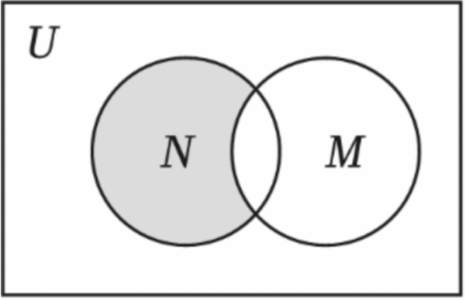
\includegraphics[width=0.30\textwidth]{figures/gao90_q6_venn.png}
\end{center}

\ifanswer
\ans{$N\cap\overline M$}
\fi

\item 已知 $a\in\R$，若关于 $x$ 的方程 $x^2-2x+a-2=0$ 有两个实根 $x_1$、$x_2$，且 $\dfrac1{x_1}+\dfrac1{x_2}=-\dfrac12$，则 $a$ 的值为\blankline[4.4em].

\ifanswer
\solbegin
\step{由于 $x_1$、$x_2$ 是 $x^2-2x+a-2=0$ 的两个实根，}
\step{由韦达定理得 $x_1x_2=a-2$，$x_1+x_2=2$，}
\step{因此 $\dfrac1{x_1}+\dfrac1{x_2}=\dfrac{x_1+x_2}{x_1x_2}=\dfrac2{a-2}=-\dfrac12$，所以 $a-2=-4$，解得 $a=-2$，}
\step{判别式 $\Delta=(-2)^2-4(a-2)=-4a+12$，当 $a=-2$ 时，$\Delta=8+12=20>0$，有两个实根，符合条件，故 $a=-2$.}
\solend
\fi

\item 如果 $-1<x<4$，$-6<y<2$，则 $2x-y$ 的取值范围是\blankline[4.4em].

\ifanswer
\solbegin
\step{因为 $-1<x<4$，$-6<y<2$，所以 $-2<2x<8$，$-2<-y<6$，}
\step{则 $-2+(-2)<2x-y<8+6$，即 $-4<2x-y<14$，}
\step{故 $2x-y$ 的取值范围为 $(-4,14)$.}
\solend
\fi

\item 集合 $A=\left\{x\left|\dfrac6{3-x}\in\Z,x\in\N\right.\right\}$，试用列举法表示集合 $A=\blankline[4.4em]$.

\ifanswer
\solbegin
\step{集合 $A=\left\{x\left|\dfrac6{3-x}\in\Z,x\in\N\right.\right\}$，所以 $3-x$ 可取的值有 $\pm1$、$\pm2$、$\pm3$、$\pm6$，}
\step{又因为 $x\in\N$，所以 $x\in\{0,1,2,4,5,6,9\}$，即 $A=\{0,1,2,4,5,6,9\}$.}
\solend
\fi

\item 不等式 $x^2-ax-b<0$ 的解集是 $(2,3)$，若关于 $x$ 的不等式组 $\begin{cases}(x-a)(3x+b)<0\\ x>t\end{cases}$ 没有实数解，则实数 $t$ 的取值范围是\blankline[4.4em].

\ifanswer
\solbegin
\step{因为等式 $x^2-ax-b<0$ 的解集是 $(2,3)$，所以 $x^2-ax-b=0$ 的根为 $2$、$3$，}
\step{所以 $2+3=a$，$2\times3=-b$，所以 $a=5$，$b=-6$，}
\step{由 $(x-a)(3x+b)=(x-5)(3x-6)<0$ 得 $2<x<5$，}
\step{若关于 $x$ 的不等式组 $\begin{cases}(x-a)(3x+b)<0\\ x>t\end{cases}$ 没有实数解，则 $t\geqslant5$.}
\solend
\fi

\item 若方程 $x^2+2x-m=0$ 有解，则 $m\geqslant a$ 为真命题，则 $a$ 的取值范围为\blankline[4.4em].

\ifanswer
\solbegin
\step{因为方程 $x^2+2x-m=0$ 有解，}
\step{所以 $\Delta=2^2-4\times1\times(-m)=4+4m\geqslant0$，解得 $m\geqslant-1$，}
\step{命题“若方程有解，则 $m\geqslant a$”为真命题，即 $\forall m\in[-1,+\infty)$，$m\geqslant a$ 恒成立，}
\step{因此 $a$ 的取值不能超过集合 $[-1,+\infty)$ 的最小值，即 $a\leqslant-1$，}
\step{综上，$a$ 的取值范围为 $(-\infty,-1]$.}
\solend
\fi

\item 设数集 $M=\left\{x\left|m\leqslant x\leqslant m+\dfrac45\right.\right\}$，$N=\left\{x\left|n-\dfrac14\leqslant x\leqslant n\right.\right\}$，且集合 $M$、$N$ 都是集合 $U=\{x\mid0\leqslant x\leqslant1\}$ 的子集，如果把 $b-a$ 称为非空集合 $\{x\mid a\leqslant x\leqslant b\}$ 的“长度”，那么集合 $M\cap N$ 的“长度”的取值范围为\blankline[4.4em].

\ifanswer
\solbegin
\step{注意到集合 $M$ 的长度为 $\dfrac45$，集合 $N$ 的长度为 $\dfrac14$，均为定值，}
\step{要使得 $M\cap N$ 的“长度”最小，则 $M$ 和 $N$ 尽可能分散到区间的两边，}
\step{长度最小为 $\dfrac45+\dfrac14-1=\dfrac1{20}$；}
\step{要使得 $M\cap N$ 的“长度”最大，则 $M$ 和 $N$ 尽可能集中，}
\step{长度最大就是集合 $N$ 的长度，为 $\dfrac14$，}
\step{故集合 $M\cap N$ 的“长度”的取值范围为 $\left[\dfrac1{20},\dfrac14\right]$.}
\solend
\fi

\end{enumerate}

\bigsec{二、选择题}

\begin{enumerate}
\setcounter{enumi}{12}

\item 设集合 $A=\{x\mid x=2k+1,k\in\Z\}$，$B=\{x\mid x=2k-1,k\in\Z\}$，则 $A$、$B$ 之间的关系是\mbox{（\quad）}

\keepwithprev
A. $B\subsetneq A$\qquad B. $A\subsetneq B$\qquad C. $A=B$\qquad D. 以上都不是

\ifanswer
\solbegin
\step{因为 $k\in\Z$，所以 $2k+1$ 与 $2k-1$ 均表示全体奇数，}
\step{即集合 $A=\{x\mid x=2k+1,k\in\Z\}$ 与 $B=\{x\mid x=2k-1,k\in\Z\}$}
\step{都表示全体奇数构成的集合，所以 $A=B$. 故选 $C$.}
\solend
\fi

\item 已知 $a$、$b\in\R$，且 $a>b$，则下列不等式中一定成立的是\mbox{（\quad）}

\keepwithprev
A. $a+1>b$\qquad B. $a>b+1$\qquad C. $a+1<b+1$\qquad D. $a-1<b-1$

\ifanswer
\solbegin
\step{因为 $a>b$，所以 $a+1>b+1$，$a-1>b-1$，故 $CD$ 错误；}
\step{因为 $a>b$，所以 $a+1>b+0$，即 $a+1>b$ 恒成立，故 $A$ 正确；}
\step{取 $a=1$，$b=0$，$B$ 显然错误.}
\step{故选 $A$.}
\solend
\fi

\item 设 $a$、$b\in\R$，“$a+b>2$ 且 $ab>1$”是“$a>1$，$b>1$”的\mbox{（\quad）}

\keepwithprev
A. 充分不必要条件\qquad B. 必要不充分条件

C. 充要条件\qquad D. 既不充分又不必要条件

\ifanswer
\solbegin
\step{因为 $a>1$ 且 $b>1$，所以 $a+b>2$ 且 $ab>1$，}
\step{若已知 $a+b>2$ 且 $ab>1$，可取 $a=\dfrac12$，$b=8$，也满足已知，}
\step{所以“$a+b>2$ 且 $ab>1$”是“$a>1$ 且 $b>1$”的必要不充分条件，故选 $B$.}
\solend
\fi

\item 设集合 $P_1=\{x\mid x^2+ax+1>0\}$，$P_2=\{x\mid x^2+ax+2>0\}$，$Q_1=\{x\mid x^2+x+b>0\}$，$Q_2=\{x\mid x^2+2x+b>0\}$，其中 $a$、$b\in\R$，下列说法中正确的是\mbox{（\quad）}

\keepwithprev
A. 对任意 $a$，$P_1$ 是 $P_2$ 的子集，对任意 $b$，$Q_1$ 不是 $Q_2$ 的子集

B. 对任意 $a$，$P_1$ 是 $P_2$ 的子集，存在 $b$，使得 $Q_1$ 是 $Q_2$ 的子集

C. 存在 $a$，使得 $P_1$ 不是 $P_2$ 的子集，对任意 $b$，$Q_1$ 不是 $Q_2$ 的子集

D. 存在 $a$，使得 $P_1$ 不是 $P_2$ 的子集，存在 $b$，使得 $Q_1$ 是 $Q_2$ 的子集

\ifanswer
\solbegin
\step{对于集合 $P_1=\{x\mid x^2+ax+1>0\}$，$P_2=\{x\mid x^2+ax+2>0\}$，}
\step{得当 $m\in P_1$ 时，即 $m^2+am+1>0$，得 $m^2+am+2>0$，}
\step{即有 $m\in P_2$，得对任意 $a$，$P_1$ 是 $P_2$ 的子集，}
\step{对于集合 $Q_1=\{x\mid x^2+x+b>0\}$，$Q_2=\{x\mid x^2+2x+b>0\}$，}
\step{当 $b=6$ 时，$Q_1=\{x\mid x^2+x+6>0\}=\R$，$Q_2=\{x\mid x^2+2x+6>0\}=\R$，}
\step{得 $Q_1$ 是 $Q_2$ 的子集，}
\step{当 $b=1$ 时，$Q_1=\{x\mid x^2+x+1>0\}=\R$，}
\step{$Q_2=\{x\mid x^2+2x+1>0\}=\{x\mid x\neq-1\}$，得 $Q_1$ 不是 $Q_2$ 的子集，}
\step{所以存在 $b$，使得 $Q_1$ 是 $Q_2$ 的子集，故选 $B$.}
\solend
\fi

\end{enumerate}

\bigsec{三、解答题}

\begin{enumerate}
\setcounter{enumi}{16}

\item 若 $a$、$b\in\R$，求关于 $x$ 的不等式 $ax\geqslant b$ 的解集.

\ansspace*[9]

\ifanswer
\solbegin
\step{当 $a>0$ 时，原不等式的解集为 $\left\{x\left|x\geqslant\dfrac ba\right.\right\}$；}
\step{当 $a<0$ 时，原不等式的解集为 $\left\{x\left|x\leqslant\dfrac ba\right.\right\}$；}
\step{当 $a=0$，$b\leqslant0$ 时，原不等式的解集为 $\R$；}
\step{当 $a=0$，$b>0$ 时，原不等式的解集为 $\varnothing$.}
\solend
\fi

\item 设集合 $A=\{x\mid x^2+3x+2=0\}$，$B=\{x\mid x^2+(m+1)x+m=0\}$.

（1）用列举法表示集合 $A$；

（2）若 $B\subseteq A$，求实数 $m$ 的值.

\ansspace*[9]

\ifanswer
\solbegin
\stepm{（1）}{集合 $A=\{x\mid x^2+3x+2=0\}$，解方程 $x^2+3x+2=0$，得 $x_1=-2$，$x_2=-1$，}
\step{所以 $A=\{-2,-1\}$.}
\stepm{（2）}{$A=\{-2,-1\}$，$B=\{x\mid x^2+(m+1)x+m=0\}=\{x\mid(x+1)(x+m)=0\}$，}
\step{$B\subseteq A$，所以 $m=1$ 或 $m=2$，所以实数 $m$ 的值为 $1$ 或 $2$.}
\solend
\fi

\item （1）设 $a$、$b$ 是两个正数. 已知 $a>b$，比较 $\dfrac{2a+b}{a+2b}$ 与 $\dfrac ab$ 的值的大小.

（2）用反证法证明：若 $a$、$b\in\R$，且 $x=a^2-2b+1$，$y=b^2-2a+1$，则 $x$、$y$ 中至少有一个不小于 $0$.

\ansspace*[12]

\ifanswer
\solbegin
\stepm{（1）}{$\dfrac{2a+b}{a+2b}-\dfrac ab=\dfrac{b(2a+b)}{b(a+2b)}-\dfrac{a(a+2b)}{b(a+2b)}=\dfrac{b(2a+b)-a(a+2b)}{b(a+2b)}$}
\step{$=\dfrac{2ab+b^2-a^2-2ab}{b(a+2b)}=\dfrac{b^2-a^2}{b(a+2b)}=\dfrac{(b+a)(b-a)}{b(a+2b)}$，}
\step{又 $a>0$，$b>0$，$a>b$，所以 $b+a>0$，$b-a<0$，$b(a+2b)>0$，}
\step{所以 $\dfrac{(b+a)(b-a)}{b(a+2b)}<0$，即 $\dfrac{2a+b}{a+2b}-\dfrac ab<0$，所以 $\dfrac{2a+b}{a+2b}<\dfrac ab$.}
\stepm{（2）}{假设 $x$、$y$ 都小于 $0$，则有 $x+y<0$，}
\step{因为 $x=a^2-2b+1$，$y=b^2-2a+1$，}
\step{所以 $x+y=(a^2-2b+1)+(b^2-2a+1)=(a^2-2a+1)+(b^2-2b+1)$}
\step{$=(a-1)^2+(b-1)^2$，}
\step{又 $a$、$b\in\R$，所以 $(a-1)^2\geqslant0$，$(b-1)^2\geqslant0$，即 $x+y\geqslant0$，}
\step{这与 $x+y<0$ 矛盾，故假设不成立，所以 $x$、$y$ 中至少有一个不小于 $0$.}
\solend
\fi

\item 已知 $m>0$，$p:(x+1)(x-5)\leqslant0$，$q:1-m\leqslant x\leqslant1+m$.

（1）若 $m=5$，$p$、$q$ 有且只有一个为真命题，求实数 $x$ 的取值范围；

（2）若 $p$ 是 $q$ 的充分不必要条件，求实数 $m$ 的取值范围.

\ansspace*[12]

\ifanswer
\solbegin
\stepm{（1）}{对于 $p:(x+1)(x-5)\leqslant0$，解得 $-1\leqslant x\leqslant5$，}
\step{若 $m=5$，则 $q:-4\leqslant x\leqslant6$，}
\step{若 $m=5$，$p$、$q$ 有且只有一个为真命题，则 $p$ 真 $q$ 假或 $p$ 假 $q$ 真，}
\step{若 $p$ 真 $q$ 假，即 $\begin{cases}-1\leqslant x\leqslant5\\ x<-4\ \text{或}\ x>6\end{cases}$，无解，}
\step{若 $p$ 假 $q$ 真，即 $\begin{cases}x<-1\ \text{或}\ x>5\\ -4\leqslant x\leqslant6\end{cases}$，解得 $-4\leqslant x<-1$ 或 $5<x\leqslant6$，}
\step{综上，$-4\leqslant x<-1$ 或 $5<x\leqslant6$，即 $x$ 的取值范围为 $[-4,-1)\cup(5,6]$；}
\stepm{（2）}{若 $p$ 是 $q$ 的充分条件，则有 $\begin{cases}1-m\leqslant-1\\ 5\leqslant1+m\end{cases}$，解得 $m\geqslant4$，}
\step{即 $m$ 的取值范围为 $[4,+\infty)$.}
\solend
\fi

\item 已知关于 $x$ 的不等式：$ax^2-(a+1)x+1<0(a\in\R)$.

（1）当 $a=-2$ 时，求不等式的解集；

（2）当 $a\geqslant0$ 时，求不等式的解集；

（3）命题 $P$：若二次不等式 $ax^2-(a+1)x+1<0$ 的解集为空集，命题 $Q:x^2-2x-a^2+a+1>0$ 对任意实数 $x$ 都成立，若 $P$、$Q$ 中至少有一个真命题，求实数 $a$ 的取值范围.

\ansspace*[14]

\ifanswer
\solbegin
\stepm{（1）}{当 $a=-2$ 时，原不等式为 $2x^2-x-1>0$，即 $(x-1)(2x+1)>0$，}
\step{解得 $x<-\dfrac12$ 或 $x>1$，所以原不等式的解集为 $\left(-\infty,-\dfrac12\right)\cup(1,+\infty)$.}
\stepm{（2）}{当 $a=0$ 时，原不等式为 $-x+1<0$，解得 $x>1$；}
\step{当 $a>0$ 时，原不等式变为 $(ax-1)(x-1)<0$，其对应方程的两根为 $\dfrac1a$，$1$，}
\step{若 $\dfrac1a<1$，即 $a>1$ 时，由 $(ax-1)(x-1)<0$ 解得 $\dfrac1a<x<1$，}
\step{若 $\dfrac1a=1$，即 $a=1$ 时，不等式 $(ax-1)(x-1)<0$ 解集为 $\varnothing$，}
\step{若 $\dfrac1a>1$，即 $0<a<1$ 时，由 $(ax-1)(x-1)<0$ 解得 $1<x<\dfrac1a$，}
\step{综上，当 $a=0$ 时，不等式的解集为 $(1,+\infty)$，}
\step{当 $0<a<1$ 时，不等式的解集为 $\left(1,\dfrac1a\right)$，}
\step{当 $a=1$ 时，不等式的解集为 $\varnothing$，}
\step{当 $a>1$ 时，不等式的解集为 $\left(\dfrac1a,1\right)$.}
\stepm{（3）}{若命题 $P$ 为真命题，}
\step{若 $a<0$，原不等式变为 $(ax-1)(x-1)<0$，其对应方程的两根为 $\dfrac1a$，$1$，}
\step{其解集为 $\left(-\infty,\dfrac1a\right)\cup(1,+\infty)$，不合题意，}
\step{当 $a\geqslant0$ 时，由（2）得当 $a=1$ 时，解集为 $\varnothing$，}
\step{所以命题 $P$ 为真命题，则 $a=1$；}
\step{命题 $Q$ 为真命题，则有相应方程的 $\Delta<0$，即 $a^2-a<0$，解得 $0<a<1$；}
\step{所以当命题 $P$、$Q$ 都为假命题时，$\begin{cases}a\leqslant0\ \text{或}\ a\geqslant1\\ a\neq1\end{cases}$，解得 $a\leqslant0$ 或 $a>1$，}
\step{所以命题 $P$、$Q$ 中至少有一个真命题，则 $0<a\leqslant1$.}
\step{所以实数 $a$ 的取值范围为 $(0,1]$.}
\solend
\fi

\end{enumerate}

\end{document}
"
%
% 原始材料：微信公众号“魔都数学加油站”文章，连载“27学年高一90”；
% 原文标题“27学年高一90——2026-2027年上海市杨思高级中学高一上10月月考”；
% 原文链接：https://mp.weixin.qq.com/s/pvQC5fkWu5Jj3C7dF3-Exw。
% 正文为 8 张 PNG 页（`原图/高一90_杨思高级中学_10月月考/01..08.png`），
% 尺寸混排（第 1、6 页为 2560×3620，其余为 4762×6735），均按页序读取。
%
% 篇幅与题号：原卷自第 3 题起编号（第 1、2 题不在原文内）。填空题 3—12（10 题）、
% 选择题 13—16（4 题）、解答题 17—21（5 题），共 19 题。
%
% 讲评版：第 6 题只印【答案】（“$N\cap\overline M$”），本稿只给 \ans{}；
% 其余 18 题印【解析】，其中选择题答案在解析末句“故选 C／A／B／B”。
% 第 6 题题干带一幅韦恩图（全集 $U$、集合 $M$、$N$ 与阴影部分），三版都出。
%
% 副标题：原卷未印副标题。本稿按内容标作“集合与常用逻辑用语、不等式”。
%
% 原卷笔误/存疑（均照录未改，正文对应处另有 % 注）：
%   ① 第 6 题的韦恩图阴影为 $N$ 中不属于 $M$ 的部分，与所印答案 $N\cap\overline M$ 一致；
%      图与答案均照录。原卷把“（请用各集合的交，并，补表示）”的逗号排作全角逗号，照录；
%   ② 第 12 题题干“如果把 $b-a$ 称为非空集合 $\{x\mid a\leqslant x\leqslant b\}$ 的‘长度’”
%      与本稿统一后的 $\R$、$\Z$、$\N$ 记号无关，原文用斜体 $R$、$Z$、$N$，按惯例改写。
%
% 与原卷的排版差异：
%   ① 原卷每题下直接印【答案】/【解析】，本稿按全稿惯例将答案与解析置于答案版；
%   ② 原卷未印副标题，本稿补出；填空横线统一排 \blankline[4.4em]；
%   ③ 原卷数集记号排斜体 $R$、$Z$、$N$，本稿按全稿惯例改用 $\R$、$\Z$、$\N$；
%   ④ 第 17—21 题的子问用行内“（1）（2）（3）”段，解析中的子问标号用 \stepm；
%   ⑤ 解答题按惯例加 \ansspace；选择题括号排 \mbox{（\quad）}；
%   ⑥ 第 6 题的韦恩图原卷排在题干右侧、文字绕排，本稿改排为题干后的居中图
%      （自原图裁切、去粉色水印后转灰度）。
%
% 行数核对：逐题数 \step/\stepm 条数，合计 94 条（Q3：2；Q4：2；Q5：1；Q6：0；
% Q7：4；Q8：3；Q9：2；Q10：4；Q11：5；Q12：6；Q13：3；Q14：4；Q15：3；Q16：9；
% Q17：4；Q18：4；Q19：10；Q20：8；Q21：20）。第 6 题只印【答案】，不计入 \step 账。
% 原卷解析的换行按语意合并，未逐行强拆。
%
\documentclass[a4paper,11pt]{article}
\usepackage{common}

\begin{document}

\examtitlest[7]{2026--2027 年杨思高级中学高一上 10 月月考}{集合与常用逻辑用语、不等式}

\bigsec{一、填空题}

\begin{enumerate}
\setcounter{enumi}{2}

\item 已知集合 $A=\{x\mid6x+a>0\}$，若 $1\notin A$，则实数 $a$ 的取值范围是\blankline[4.4em].

\ifanswer
\solbegin
\step{集合 $A=\{x\mid6x+a>0\}$，若 $1\notin A$，则 $6+a\leqslant0$ 恒成立，故 $a\leqslant-6$，}
\step{故实数 $a$ 的取值范围是 $(-\infty,-6]$.}
\solend
\fi

\item 设全集 $U=\R$，集合 $A=\{x\mid-1\leqslant x\leqslant1\}$，$B=\{x\mid0<x<2\}$，则 $\overline{A\cup B}=\blankline[4.4em]$.

\ifanswer
\solbegin
\step{$B=\{x\mid0<x<2\}$，$A=\{x\mid-1\leqslant x\leqslant1\}$，所以 $A\cup B=\{x\mid-1\leqslant x<2\}$，}
\step{又因为全集 $U=\R$，所以 $\overline{A\cup B}=(-\infty,-1)\cup[2,+\infty)$.}
\solend
\fi

\item 集合 $A=\{(x,y)\mid y=-x\}$，$B=\{(x,y)\mid y=2x-4\}$，则 $A\cap B=\blankline[4.4em]$.

\ifanswer
\solbegin
\step{联立 $\begin{cases}y=-x\\ y=2x-4\end{cases}$，解得 $\begin{cases}x=\dfrac43\\[0.2em] y=-\dfrac43\end{cases}$，即 $A\cap B=\left\{\left(\dfrac43,-\dfrac43\right)\right\}$.}
\solend
\fi

\item 设 $U$ 是全集，$M$、$N$ 是 $U$ 的子集，则图中阴影部分所表示的集合是\blankline[4.4em].

（请用各集合的交，并，补表示）

\begin{center}
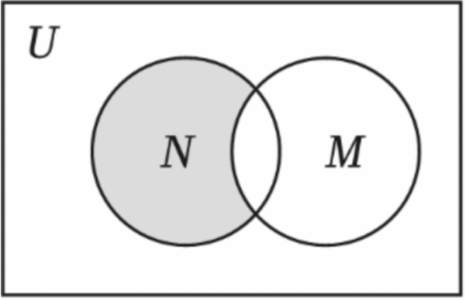
\includegraphics[width=0.30\textwidth]{figures/gao90_q6_venn.png}
\end{center}

\ifanswer
\ans{$N\cap\overline M$}
\fi

\item 已知 $a\in\R$，若关于 $x$ 的方程 $x^2-2x+a-2=0$ 有两个实根 $x_1$、$x_2$，且 $\dfrac1{x_1}+\dfrac1{x_2}=-\dfrac12$，则 $a$ 的值为\blankline[4.4em].

\ifanswer
\solbegin
\step{由于 $x_1$、$x_2$ 是 $x^2-2x+a-2=0$ 的两个实根，}
\step{由韦达定理得 $x_1x_2=a-2$，$x_1+x_2=2$，}
\step{因此 $\dfrac1{x_1}+\dfrac1{x_2}=\dfrac{x_1+x_2}{x_1x_2}=\dfrac2{a-2}=-\dfrac12$，所以 $a-2=-4$，解得 $a=-2$，}
\step{判别式 $\Delta=(-2)^2-4(a-2)=-4a+12$，当 $a=-2$ 时，$\Delta=8+12=20>0$，有两个实根，符合条件，故 $a=-2$.}
\solend
\fi

\item 如果 $-1<x<4$，$-6<y<2$，则 $2x-y$ 的取值范围是\blankline[4.4em].

\ifanswer
\solbegin
\step{因为 $-1<x<4$，$-6<y<2$，所以 $-2<2x<8$，$-2<-y<6$，}
\step{则 $-2+(-2)<2x-y<8+6$，即 $-4<2x-y<14$，}
\step{故 $2x-y$ 的取值范围为 $(-4,14)$.}
\solend
\fi

\item 集合 $A=\left\{x\left|\dfrac6{3-x}\in\Z,x\in\N\right.\right\}$，试用列举法表示集合 $A=\blankline[4.4em]$.

\ifanswer
\solbegin
\step{集合 $A=\left\{x\left|\dfrac6{3-x}\in\Z,x\in\N\right.\right\}$，所以 $3-x$ 可取的值有 $\pm1$、$\pm2$、$\pm3$、$\pm6$，}
\step{又因为 $x\in\N$，所以 $x\in\{0,1,2,4,5,6,9\}$，即 $A=\{0,1,2,4,5,6,9\}$.}
\solend
\fi

\item 不等式 $x^2-ax-b<0$ 的解集是 $(2,3)$，若关于 $x$ 的不等式组 $\begin{cases}(x-a)(3x+b)<0\\ x>t\end{cases}$ 没有实数解，则实数 $t$ 的取值范围是\blankline[4.4em].

\ifanswer
\solbegin
\step{因为等式 $x^2-ax-b<0$ 的解集是 $(2,3)$，所以 $x^2-ax-b=0$ 的根为 $2$、$3$，}
\step{所以 $2+3=a$，$2\times3=-b$，所以 $a=5$，$b=-6$，}
\step{由 $(x-a)(3x+b)=(x-5)(3x-6)<0$ 得 $2<x<5$，}
\step{若关于 $x$ 的不等式组 $\begin{cases}(x-a)(3x+b)<0\\ x>t\end{cases}$ 没有实数解，则 $t\geqslant5$.}
\solend
\fi

\item 若方程 $x^2+2x-m=0$ 有解，则 $m\geqslant a$ 为真命题，则 $a$ 的取值范围为\blankline[4.4em].

\ifanswer
\solbegin
\step{因为方程 $x^2+2x-m=0$ 有解，}
\step{所以 $\Delta=2^2-4\times1\times(-m)=4+4m\geqslant0$，解得 $m\geqslant-1$，}
\step{命题“若方程有解，则 $m\geqslant a$”为真命题，即 $\forall m\in[-1,+\infty)$，$m\geqslant a$ 恒成立，}
\step{因此 $a$ 的取值不能超过集合 $[-1,+\infty)$ 的最小值，即 $a\leqslant-1$，}
\step{综上，$a$ 的取值范围为 $(-\infty,-1]$.}
\solend
\fi

\item 设数集 $M=\left\{x\left|m\leqslant x\leqslant m+\dfrac45\right.\right\}$，$N=\left\{x\left|n-\dfrac14\leqslant x\leqslant n\right.\right\}$，且集合 $M$、$N$ 都是集合 $U=\{x\mid0\leqslant x\leqslant1\}$ 的子集，如果把 $b-a$ 称为非空集合 $\{x\mid a\leqslant x\leqslant b\}$ 的“长度”，那么集合 $M\cap N$ 的“长度”的取值范围为\blankline[4.4em].

\ifanswer
\solbegin
\step{注意到集合 $M$ 的长度为 $\dfrac45$，集合 $N$ 的长度为 $\dfrac14$，均为定值，}
\step{要使得 $M\cap N$ 的“长度”最小，则 $M$ 和 $N$ 尽可能分散到区间的两边，}
\step{长度最小为 $\dfrac45+\dfrac14-1=\dfrac1{20}$；}
\step{要使得 $M\cap N$ 的“长度”最大，则 $M$ 和 $N$ 尽可能集中，}
\step{长度最大就是集合 $N$ 的长度，为 $\dfrac14$，}
\step{故集合 $M\cap N$ 的“长度”的取值范围为 $\left[\dfrac1{20},\dfrac14\right]$.}
\solend
\fi

\end{enumerate}

\bigsec{二、选择题}

\begin{enumerate}
\setcounter{enumi}{12}

\item 设集合 $A=\{x\mid x=2k+1,k\in\Z\}$，$B=\{x\mid x=2k-1,k\in\Z\}$，则 $A$、$B$ 之间的关系是\mbox{（\quad）}

\keepwithprev
A. $B\subsetneq A$\qquad B. $A\subsetneq B$\qquad C. $A=B$\qquad D. 以上都不是

\ifanswer
\solbegin
\step{因为 $k\in\Z$，所以 $2k+1$ 与 $2k-1$ 均表示全体奇数，}
\step{即集合 $A=\{x\mid x=2k+1,k\in\Z\}$ 与 $B=\{x\mid x=2k-1,k\in\Z\}$}
\step{都表示全体奇数构成的集合，所以 $A=B$. 故选 $C$.}
\solend
\fi

\item 已知 $a$、$b\in\R$，且 $a>b$，则下列不等式中一定成立的是\mbox{（\quad）}

\keepwithprev
A. $a+1>b$\qquad B. $a>b+1$\qquad C. $a+1<b+1$\qquad D. $a-1<b-1$

\ifanswer
\solbegin
\step{因为 $a>b$，所以 $a+1>b+1$，$a-1>b-1$，故 $CD$ 错误；}
\step{因为 $a>b$，所以 $a+1>b+0$，即 $a+1>b$ 恒成立，故 $A$ 正确；}
\step{取 $a=1$，$b=0$，$B$ 显然错误.}
\step{故选 $A$.}
\solend
\fi

\item 设 $a$、$b\in\R$，“$a+b>2$ 且 $ab>1$”是“$a>1$，$b>1$”的\mbox{（\quad）}

\keepwithprev
A. 充分不必要条件\qquad B. 必要不充分条件

C. 充要条件\qquad D. 既不充分又不必要条件

\ifanswer
\solbegin
\step{因为 $a>1$ 且 $b>1$，所以 $a+b>2$ 且 $ab>1$，}
\step{若已知 $a+b>2$ 且 $ab>1$，可取 $a=\dfrac12$，$b=8$，也满足已知，}
\step{所以“$a+b>2$ 且 $ab>1$”是“$a>1$ 且 $b>1$”的必要不充分条件，故选 $B$.}
\solend
\fi

\item 设集合 $P_1=\{x\mid x^2+ax+1>0\}$，$P_2=\{x\mid x^2+ax+2>0\}$，$Q_1=\{x\mid x^2+x+b>0\}$，$Q_2=\{x\mid x^2+2x+b>0\}$，其中 $a$、$b\in\R$，下列说法中正确的是\mbox{（\quad）}

\keepwithprev
A. 对任意 $a$，$P_1$ 是 $P_2$ 的子集，对任意 $b$，$Q_1$ 不是 $Q_2$ 的子集

B. 对任意 $a$，$P_1$ 是 $P_2$ 的子集，存在 $b$，使得 $Q_1$ 是 $Q_2$ 的子集

C. 存在 $a$，使得 $P_1$ 不是 $P_2$ 的子集，对任意 $b$，$Q_1$ 不是 $Q_2$ 的子集

D. 存在 $a$，使得 $P_1$ 不是 $P_2$ 的子集，存在 $b$，使得 $Q_1$ 是 $Q_2$ 的子集

\ifanswer
\solbegin
\step{对于集合 $P_1=\{x\mid x^2+ax+1>0\}$，$P_2=\{x\mid x^2+ax+2>0\}$，}
\step{得当 $m\in P_1$ 时，即 $m^2+am+1>0$，得 $m^2+am+2>0$，}
\step{即有 $m\in P_2$，得对任意 $a$，$P_1$ 是 $P_2$ 的子集，}
\step{对于集合 $Q_1=\{x\mid x^2+x+b>0\}$，$Q_2=\{x\mid x^2+2x+b>0\}$，}
\step{当 $b=6$ 时，$Q_1=\{x\mid x^2+x+6>0\}=\R$，$Q_2=\{x\mid x^2+2x+6>0\}=\R$，}
\step{得 $Q_1$ 是 $Q_2$ 的子集，}
\step{当 $b=1$ 时，$Q_1=\{x\mid x^2+x+1>0\}=\R$，}
\step{$Q_2=\{x\mid x^2+2x+1>0\}=\{x\mid x\neq-1\}$，得 $Q_1$ 不是 $Q_2$ 的子集，}
\step{所以存在 $b$，使得 $Q_1$ 是 $Q_2$ 的子集，故选 $B$.}
\solend
\fi

\end{enumerate}

\bigsec{三、解答题}

\begin{enumerate}
\setcounter{enumi}{16}

\item 若 $a$、$b\in\R$，求关于 $x$ 的不等式 $ax\geqslant b$ 的解集.

\ansspace*[9]

\ifanswer
\solbegin
\step{当 $a>0$ 时，原不等式的解集为 $\left\{x\left|x\geqslant\dfrac ba\right.\right\}$；}
\step{当 $a<0$ 时，原不等式的解集为 $\left\{x\left|x\leqslant\dfrac ba\right.\right\}$；}
\step{当 $a=0$，$b\leqslant0$ 时，原不等式的解集为 $\R$；}
\step{当 $a=0$，$b>0$ 时，原不等式的解集为 $\varnothing$.}
\solend
\fi

\item 设集合 $A=\{x\mid x^2+3x+2=0\}$，$B=\{x\mid x^2+(m+1)x+m=0\}$.

（1）用列举法表示集合 $A$；

（2）若 $B\subseteq A$，求实数 $m$ 的值.

\ansspace*[9]

\ifanswer
\solbegin
\stepm{（1）}{集合 $A=\{x\mid x^2+3x+2=0\}$，解方程 $x^2+3x+2=0$，得 $x_1=-2$，$x_2=-1$，}
\step{所以 $A=\{-2,-1\}$.}
\stepm{（2）}{$A=\{-2,-1\}$，$B=\{x\mid x^2+(m+1)x+m=0\}=\{x\mid(x+1)(x+m)=0\}$，}
\step{$B\subseteq A$，所以 $m=1$ 或 $m=2$，所以实数 $m$ 的值为 $1$ 或 $2$.}
\solend
\fi

\item （1）设 $a$、$b$ 是两个正数. 已知 $a>b$，比较 $\dfrac{2a+b}{a+2b}$ 与 $\dfrac ab$ 的值的大小.

（2）用反证法证明：若 $a$、$b\in\R$，且 $x=a^2-2b+1$，$y=b^2-2a+1$，则 $x$、$y$ 中至少有一个不小于 $0$.

\ansspace*[12]

\ifanswer
\solbegin
\stepm{（1）}{$\dfrac{2a+b}{a+2b}-\dfrac ab=\dfrac{b(2a+b)}{b(a+2b)}-\dfrac{a(a+2b)}{b(a+2b)}=\dfrac{b(2a+b)-a(a+2b)}{b(a+2b)}$}
\step{$=\dfrac{2ab+b^2-a^2-2ab}{b(a+2b)}=\dfrac{b^2-a^2}{b(a+2b)}=\dfrac{(b+a)(b-a)}{b(a+2b)}$，}
\step{又 $a>0$，$b>0$，$a>b$，所以 $b+a>0$，$b-a<0$，$b(a+2b)>0$，}
\step{所以 $\dfrac{(b+a)(b-a)}{b(a+2b)}<0$，即 $\dfrac{2a+b}{a+2b}-\dfrac ab<0$，所以 $\dfrac{2a+b}{a+2b}<\dfrac ab$.}
\stepm{（2）}{假设 $x$、$y$ 都小于 $0$，则有 $x+y<0$，}
\step{因为 $x=a^2-2b+1$，$y=b^2-2a+1$，}
\step{所以 $x+y=(a^2-2b+1)+(b^2-2a+1)=(a^2-2a+1)+(b^2-2b+1)$}
\step{$=(a-1)^2+(b-1)^2$，}
\step{又 $a$、$b\in\R$，所以 $(a-1)^2\geqslant0$，$(b-1)^2\geqslant0$，即 $x+y\geqslant0$，}
\step{这与 $x+y<0$ 矛盾，故假设不成立，所以 $x$、$y$ 中至少有一个不小于 $0$.}
\solend
\fi

\item 已知 $m>0$，$p:(x+1)(x-5)\leqslant0$，$q:1-m\leqslant x\leqslant1+m$.

（1）若 $m=5$，$p$、$q$ 有且只有一个为真命题，求实数 $x$ 的取值范围；

（2）若 $p$ 是 $q$ 的充分不必要条件，求实数 $m$ 的取值范围.

\ansspace*[12]

\ifanswer
\solbegin
\stepm{（1）}{对于 $p:(x+1)(x-5)\leqslant0$，解得 $-1\leqslant x\leqslant5$，}
\step{若 $m=5$，则 $q:-4\leqslant x\leqslant6$，}
\step{若 $m=5$，$p$、$q$ 有且只有一个为真命题，则 $p$ 真 $q$ 假或 $p$ 假 $q$ 真，}
\step{若 $p$ 真 $q$ 假，即 $\begin{cases}-1\leqslant x\leqslant5\\ x<-4\ \text{或}\ x>6\end{cases}$，无解，}
\step{若 $p$ 假 $q$ 真，即 $\begin{cases}x<-1\ \text{或}\ x>5\\ -4\leqslant x\leqslant6\end{cases}$，解得 $-4\leqslant x<-1$ 或 $5<x\leqslant6$，}
\step{综上，$-4\leqslant x<-1$ 或 $5<x\leqslant6$，即 $x$ 的取值范围为 $[-4,-1)\cup(5,6]$；}
\stepm{（2）}{若 $p$ 是 $q$ 的充分条件，则有 $\begin{cases}1-m\leqslant-1\\ 5\leqslant1+m\end{cases}$，解得 $m\geqslant4$，}
\step{即 $m$ 的取值范围为 $[4,+\infty)$.}
\solend
\fi

\item 已知关于 $x$ 的不等式：$ax^2-(a+1)x+1<0(a\in\R)$.

（1）当 $a=-2$ 时，求不等式的解集；

（2）当 $a\geqslant0$ 时，求不等式的解集；

（3）命题 $P$：若二次不等式 $ax^2-(a+1)x+1<0$ 的解集为空集，命题 $Q:x^2-2x-a^2+a+1>0$ 对任意实数 $x$ 都成立，若 $P$、$Q$ 中至少有一个真命题，求实数 $a$ 的取值范围.

\ansspace*[14]

\ifanswer
\solbegin
\stepm{（1）}{当 $a=-2$ 时，原不等式为 $2x^2-x-1>0$，即 $(x-1)(2x+1)>0$，}
\step{解得 $x<-\dfrac12$ 或 $x>1$，所以原不等式的解集为 $\left(-\infty,-\dfrac12\right)\cup(1,+\infty)$.}
\stepm{（2）}{当 $a=0$ 时，原不等式为 $-x+1<0$，解得 $x>1$；}
\step{当 $a>0$ 时，原不等式变为 $(ax-1)(x-1)<0$，其对应方程的两根为 $\dfrac1a$，$1$，}
\step{若 $\dfrac1a<1$，即 $a>1$ 时，由 $(ax-1)(x-1)<0$ 解得 $\dfrac1a<x<1$，}
\step{若 $\dfrac1a=1$，即 $a=1$ 时，不等式 $(ax-1)(x-1)<0$ 解集为 $\varnothing$，}
\step{若 $\dfrac1a>1$，即 $0<a<1$ 时，由 $(ax-1)(x-1)<0$ 解得 $1<x<\dfrac1a$，}
\step{综上，当 $a=0$ 时，不等式的解集为 $(1,+\infty)$，}
\step{当 $0<a<1$ 时，不等式的解集为 $\left(1,\dfrac1a\right)$，}
\step{当 $a=1$ 时，不等式的解集为 $\varnothing$，}
\step{当 $a>1$ 时，不等式的解集为 $\left(\dfrac1a,1\right)$.}
\stepm{（3）}{若命题 $P$ 为真命题，}
\step{若 $a<0$，原不等式变为 $(ax-1)(x-1)<0$，其对应方程的两根为 $\dfrac1a$，$1$，}
\step{其解集为 $\left(-\infty,\dfrac1a\right)\cup(1,+\infty)$，不合题意，}
\step{当 $a\geqslant0$ 时，由（2）得当 $a=1$ 时，解集为 $\varnothing$，}
\step{所以命题 $P$ 为真命题，则 $a=1$；}
\step{命题 $Q$ 为真命题，则有相应方程的 $\Delta<0$，即 $a^2-a<0$，解得 $0<a<1$；}
\step{所以当命题 $P$、$Q$ 都为假命题时，$\begin{cases}a\leqslant0\ \text{或}\ a\geqslant1\\ a\neq1\end{cases}$，解得 $a\leqslant0$ 或 $a>1$，}
\step{所以命题 $P$、$Q$ 中至少有一个真命题，则 $0<a\leqslant1$.}
\step{所以实数 $a$ 的取值范围为 $(0,1]$.}
\solend
\fi

\end{enumerate}

\end{document}
"
%
% 原始材料：微信公众号“魔都数学加油站”文章，连载“27学年高一90”；
% 原文标题“27学年高一90——2026-2027年上海市杨思高级中学高一上10月月考”；
% 原文链接：https://mp.weixin.qq.com/s/pvQC5fkWu5Jj3C7dF3-Exw。
% 正文为 8 张 PNG 页（`原图/高一90_杨思高级中学_10月月考/01..08.png`），
% 尺寸混排（第 1、6 页为 2560×3620，其余为 4762×6735），均按页序读取。
%
% 篇幅与题号：原卷自第 3 题起编号（第 1、2 题不在原文内）。填空题 3—12（10 题）、
% 选择题 13—16（4 题）、解答题 17—21（5 题），共 19 题。
%
% 讲评版：第 6 题只印【答案】（“$N\cap\overline M$”），本稿只给 \ans{}；
% 其余 18 题印【解析】，其中选择题答案在解析末句“故选 C／A／B／B”。
% 第 6 题题干带一幅韦恩图（全集 $U$、集合 $M$、$N$ 与阴影部分），三版都出。
%
% 副标题：原卷未印副标题。本稿按内容标作“集合与常用逻辑用语、不等式”。
%
% 原卷笔误/存疑（均照录未改，正文对应处另有 % 注）：
%   ① 第 6 题的韦恩图阴影为 $N$ 中不属于 $M$ 的部分，与所印答案 $N\cap\overline M$ 一致；
%      图与答案均照录。原卷把“（请用各集合的交，并，补表示）”的逗号排作全角逗号，照录；
%   ② 第 12 题题干“如果把 $b-a$ 称为非空集合 $\{x\mid a\leqslant x\leqslant b\}$ 的‘长度’”
%      与本稿统一后的 $\R$、$\Z$、$\N$ 记号无关，原文用斜体 $R$、$Z$、$N$，按惯例改写。
%
% 与原卷的排版差异：
%   ① 原卷每题下直接印【答案】/【解析】，本稿按全稿惯例将答案与解析置于答案版；
%   ② 原卷未印副标题，本稿补出；填空横线统一排 \blankline[4.4em]；
%   ③ 原卷数集记号排斜体 $R$、$Z$、$N$，本稿按全稿惯例改用 $\R$、$\Z$、$\N$；
%   ④ 第 17—21 题的子问用行内“（1）（2）（3）”段，解析中的子问标号用 \stepm；
%   ⑤ 解答题按惯例加 \ansspace；选择题括号排 \mbox{（\quad）}；
%   ⑥ 第 6 题的韦恩图原卷排在题干右侧、文字绕排，本稿改排为题干后的居中图
%      （自原图裁切、去粉色水印后转灰度）。
%
% 行数核对：逐题数 \step/\stepm 条数，合计 94 条（Q3：2；Q4：2；Q5：1；Q6：0；
% Q7：4；Q8：3；Q9：2；Q10：4；Q11：5；Q12：6；Q13：3；Q14：4；Q15：3；Q16：9；
% Q17：4；Q18：4；Q19：10；Q20：8；Q21：20）。第 6 题只印【答案】，不计入 \step 账。
% 原卷解析的换行按语意合并，未逐行强拆。
%
\documentclass[a4paper,11pt]{article}
\usepackage{common}

\begin{document}

\examtitlest[7]{2026--2027 年杨思高级中学高一上 10 月月考}{集合与常用逻辑用语、不等式}

\bigsec{一、填空题}

\begin{enumerate}
\setcounter{enumi}{2}

\item 已知集合 $A=\{x\mid6x+a>0\}$，若 $1\notin A$，则实数 $a$ 的取值范围是\blankline[4.4em].

\ifanswer
\solbegin
\step{集合 $A=\{x\mid6x+a>0\}$，若 $1\notin A$，则 $6+a\leqslant0$ 恒成立，故 $a\leqslant-6$，}
\step{故实数 $a$ 的取值范围是 $(-\infty,-6]$.}
\solend
\fi

\item 设全集 $U=\R$，集合 $A=\{x\mid-1\leqslant x\leqslant1\}$，$B=\{x\mid0<x<2\}$，则 $\overline{A\cup B}=\blankline[4.4em]$.

\ifanswer
\solbegin
\step{$B=\{x\mid0<x<2\}$，$A=\{x\mid-1\leqslant x\leqslant1\}$，所以 $A\cup B=\{x\mid-1\leqslant x<2\}$，}
\step{又因为全集 $U=\R$，所以 $\overline{A\cup B}=(-\infty,-1)\cup[2,+\infty)$.}
\solend
\fi

\item 集合 $A=\{(x,y)\mid y=-x\}$，$B=\{(x,y)\mid y=2x-4\}$，则 $A\cap B=\blankline[4.4em]$.

\ifanswer
\solbegin
\step{联立 $\begin{cases}y=-x\\ y=2x-4\end{cases}$，解得 $\begin{cases}x=\dfrac43\\[0.2em] y=-\dfrac43\end{cases}$，即 $A\cap B=\left\{\left(\dfrac43,-\dfrac43\right)\right\}$.}
\solend
\fi

\item 设 $U$ 是全集，$M$、$N$ 是 $U$ 的子集，则图中阴影部分所表示的集合是\blankline[4.4em].

（请用各集合的交，并，补表示）

\begin{center}
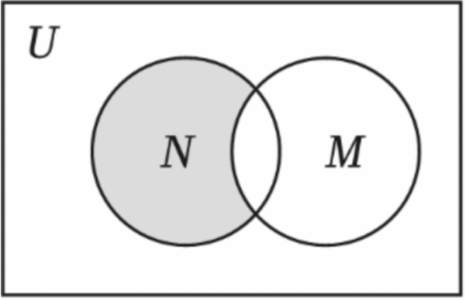
\includegraphics[width=0.30\textwidth]{figures/gao90_q6_venn.png}
\end{center}

\ifanswer
\ans{$N\cap\overline M$}
\fi

\item 已知 $a\in\R$，若关于 $x$ 的方程 $x^2-2x+a-2=0$ 有两个实根 $x_1$、$x_2$，且 $\dfrac1{x_1}+\dfrac1{x_2}=-\dfrac12$，则 $a$ 的值为\blankline[4.4em].

\ifanswer
\solbegin
\step{由于 $x_1$、$x_2$ 是 $x^2-2x+a-2=0$ 的两个实根，}
\step{由韦达定理得 $x_1x_2=a-2$，$x_1+x_2=2$，}
\step{因此 $\dfrac1{x_1}+\dfrac1{x_2}=\dfrac{x_1+x_2}{x_1x_2}=\dfrac2{a-2}=-\dfrac12$，所以 $a-2=-4$，解得 $a=-2$，}
\step{判别式 $\Delta=(-2)^2-4(a-2)=-4a+12$，当 $a=-2$ 时，$\Delta=8+12=20>0$，有两个实根，符合条件，故 $a=-2$.}
\solend
\fi

\item 如果 $-1<x<4$，$-6<y<2$，则 $2x-y$ 的取值范围是\blankline[4.4em].

\ifanswer
\solbegin
\step{因为 $-1<x<4$，$-6<y<2$，所以 $-2<2x<8$，$-2<-y<6$，}
\step{则 $-2+(-2)<2x-y<8+6$，即 $-4<2x-y<14$，}
\step{故 $2x-y$ 的取值范围为 $(-4,14)$.}
\solend
\fi

\item 集合 $A=\left\{x\left|\dfrac6{3-x}\in\Z,x\in\N\right.\right\}$，试用列举法表示集合 $A=\blankline[4.4em]$.

\ifanswer
\solbegin
\step{集合 $A=\left\{x\left|\dfrac6{3-x}\in\Z,x\in\N\right.\right\}$，所以 $3-x$ 可取的值有 $\pm1$、$\pm2$、$\pm3$、$\pm6$，}
\step{又因为 $x\in\N$，所以 $x\in\{0,1,2,4,5,6,9\}$，即 $A=\{0,1,2,4,5,6,9\}$.}
\solend
\fi

\item 不等式 $x^2-ax-b<0$ 的解集是 $(2,3)$，若关于 $x$ 的不等式组 $\begin{cases}(x-a)(3x+b)<0\\ x>t\end{cases}$ 没有实数解，则实数 $t$ 的取值范围是\blankline[4.4em].

\ifanswer
\solbegin
\step{因为等式 $x^2-ax-b<0$ 的解集是 $(2,3)$，所以 $x^2-ax-b=0$ 的根为 $2$、$3$，}
\step{所以 $2+3=a$，$2\times3=-b$，所以 $a=5$，$b=-6$，}
\step{由 $(x-a)(3x+b)=(x-5)(3x-6)<0$ 得 $2<x<5$，}
\step{若关于 $x$ 的不等式组 $\begin{cases}(x-a)(3x+b)<0\\ x>t\end{cases}$ 没有实数解，则 $t\geqslant5$.}
\solend
\fi

\item 若方程 $x^2+2x-m=0$ 有解，则 $m\geqslant a$ 为真命题，则 $a$ 的取值范围为\blankline[4.4em].

\ifanswer
\solbegin
\step{因为方程 $x^2+2x-m=0$ 有解，}
\step{所以 $\Delta=2^2-4\times1\times(-m)=4+4m\geqslant0$，解得 $m\geqslant-1$，}
\step{命题“若方程有解，则 $m\geqslant a$”为真命题，即 $\forall m\in[-1,+\infty)$，$m\geqslant a$ 恒成立，}
\step{因此 $a$ 的取值不能超过集合 $[-1,+\infty)$ 的最小值，即 $a\leqslant-1$，}
\step{综上，$a$ 的取值范围为 $(-\infty,-1]$.}
\solend
\fi

\item 设数集 $M=\left\{x\left|m\leqslant x\leqslant m+\dfrac45\right.\right\}$，$N=\left\{x\left|n-\dfrac14\leqslant x\leqslant n\right.\right\}$，且集合 $M$、$N$ 都是集合 $U=\{x\mid0\leqslant x\leqslant1\}$ 的子集，如果把 $b-a$ 称为非空集合 $\{x\mid a\leqslant x\leqslant b\}$ 的“长度”，那么集合 $M\cap N$ 的“长度”的取值范围为\blankline[4.4em].

\ifanswer
\solbegin
\step{注意到集合 $M$ 的长度为 $\dfrac45$，集合 $N$ 的长度为 $\dfrac14$，均为定值，}
\step{要使得 $M\cap N$ 的“长度”最小，则 $M$ 和 $N$ 尽可能分散到区间的两边，}
\step{长度最小为 $\dfrac45+\dfrac14-1=\dfrac1{20}$；}
\step{要使得 $M\cap N$ 的“长度”最大，则 $M$ 和 $N$ 尽可能集中，}
\step{长度最大就是集合 $N$ 的长度，为 $\dfrac14$，}
\step{故集合 $M\cap N$ 的“长度”的取值范围为 $\left[\dfrac1{20},\dfrac14\right]$.}
\solend
\fi

\end{enumerate}

\bigsec{二、选择题}

\begin{enumerate}
\setcounter{enumi}{12}

\item 设集合 $A=\{x\mid x=2k+1,k\in\Z\}$，$B=\{x\mid x=2k-1,k\in\Z\}$，则 $A$、$B$ 之间的关系是\mbox{（\quad）}

\keepwithprev
A. $B\subsetneq A$\qquad B. $A\subsetneq B$\qquad C. $A=B$\qquad D. 以上都不是

\ifanswer
\solbegin
\step{因为 $k\in\Z$，所以 $2k+1$ 与 $2k-1$ 均表示全体奇数，}
\step{即集合 $A=\{x\mid x=2k+1,k\in\Z\}$ 与 $B=\{x\mid x=2k-1,k\in\Z\}$}
\step{都表示全体奇数构成的集合，所以 $A=B$. 故选 $C$.}
\solend
\fi

\item 已知 $a$、$b\in\R$，且 $a>b$，则下列不等式中一定成立的是\mbox{（\quad）}

\keepwithprev
A. $a+1>b$\qquad B. $a>b+1$\qquad C. $a+1<b+1$\qquad D. $a-1<b-1$

\ifanswer
\solbegin
\step{因为 $a>b$，所以 $a+1>b+1$，$a-1>b-1$，故 $CD$ 错误；}
\step{因为 $a>b$，所以 $a+1>b+0$，即 $a+1>b$ 恒成立，故 $A$ 正确；}
\step{取 $a=1$，$b=0$，$B$ 显然错误.}
\step{故选 $A$.}
\solend
\fi

\item 设 $a$、$b\in\R$，“$a+b>2$ 且 $ab>1$”是“$a>1$，$b>1$”的\mbox{（\quad）}

\keepwithprev
A. 充分不必要条件\qquad B. 必要不充分条件

C. 充要条件\qquad D. 既不充分又不必要条件

\ifanswer
\solbegin
\step{因为 $a>1$ 且 $b>1$，所以 $a+b>2$ 且 $ab>1$，}
\step{若已知 $a+b>2$ 且 $ab>1$，可取 $a=\dfrac12$，$b=8$，也满足已知，}
\step{所以“$a+b>2$ 且 $ab>1$”是“$a>1$ 且 $b>1$”的必要不充分条件，故选 $B$.}
\solend
\fi

\item 设集合 $P_1=\{x\mid x^2+ax+1>0\}$，$P_2=\{x\mid x^2+ax+2>0\}$，$Q_1=\{x\mid x^2+x+b>0\}$，$Q_2=\{x\mid x^2+2x+b>0\}$，其中 $a$、$b\in\R$，下列说法中正确的是\mbox{（\quad）}

\keepwithprev
A. 对任意 $a$，$P_1$ 是 $P_2$ 的子集，对任意 $b$，$Q_1$ 不是 $Q_2$ 的子集

B. 对任意 $a$，$P_1$ 是 $P_2$ 的子集，存在 $b$，使得 $Q_1$ 是 $Q_2$ 的子集

C. 存在 $a$，使得 $P_1$ 不是 $P_2$ 的子集，对任意 $b$，$Q_1$ 不是 $Q_2$ 的子集

D. 存在 $a$，使得 $P_1$ 不是 $P_2$ 的子集，存在 $b$，使得 $Q_1$ 是 $Q_2$ 的子集

\ifanswer
\solbegin
\step{对于集合 $P_1=\{x\mid x^2+ax+1>0\}$，$P_2=\{x\mid x^2+ax+2>0\}$，}
\step{得当 $m\in P_1$ 时，即 $m^2+am+1>0$，得 $m^2+am+2>0$，}
\step{即有 $m\in P_2$，得对任意 $a$，$P_1$ 是 $P_2$ 的子集，}
\step{对于集合 $Q_1=\{x\mid x^2+x+b>0\}$，$Q_2=\{x\mid x^2+2x+b>0\}$，}
\step{当 $b=6$ 时，$Q_1=\{x\mid x^2+x+6>0\}=\R$，$Q_2=\{x\mid x^2+2x+6>0\}=\R$，}
\step{得 $Q_1$ 是 $Q_2$ 的子集，}
\step{当 $b=1$ 时，$Q_1=\{x\mid x^2+x+1>0\}=\R$，}
\step{$Q_2=\{x\mid x^2+2x+1>0\}=\{x\mid x\neq-1\}$，得 $Q_1$ 不是 $Q_2$ 的子集，}
\step{所以存在 $b$，使得 $Q_1$ 是 $Q_2$ 的子集，故选 $B$.}
\solend
\fi

\end{enumerate}

\bigsec{三、解答题}

\begin{enumerate}
\setcounter{enumi}{16}

\item 若 $a$、$b\in\R$，求关于 $x$ 的不等式 $ax\geqslant b$ 的解集.

\ansspace*[9]

\ifanswer
\solbegin
\step{当 $a>0$ 时，原不等式的解集为 $\left\{x\left|x\geqslant\dfrac ba\right.\right\}$；}
\step{当 $a<0$ 时，原不等式的解集为 $\left\{x\left|x\leqslant\dfrac ba\right.\right\}$；}
\step{当 $a=0$，$b\leqslant0$ 时，原不等式的解集为 $\R$；}
\step{当 $a=0$，$b>0$ 时，原不等式的解集为 $\varnothing$.}
\solend
\fi

\item 设集合 $A=\{x\mid x^2+3x+2=0\}$，$B=\{x\mid x^2+(m+1)x+m=0\}$.

（1）用列举法表示集合 $A$；

（2）若 $B\subseteq A$，求实数 $m$ 的值.

\ansspace*[9]

\ifanswer
\solbegin
\stepm{（1）}{集合 $A=\{x\mid x^2+3x+2=0\}$，解方程 $x^2+3x+2=0$，得 $x_1=-2$，$x_2=-1$，}
\step{所以 $A=\{-2,-1\}$.}
\stepm{（2）}{$A=\{-2,-1\}$，$B=\{x\mid x^2+(m+1)x+m=0\}=\{x\mid(x+1)(x+m)=0\}$，}
\step{$B\subseteq A$，所以 $m=1$ 或 $m=2$，所以实数 $m$ 的值为 $1$ 或 $2$.}
\solend
\fi

\item （1）设 $a$、$b$ 是两个正数. 已知 $a>b$，比较 $\dfrac{2a+b}{a+2b}$ 与 $\dfrac ab$ 的值的大小.

（2）用反证法证明：若 $a$、$b\in\R$，且 $x=a^2-2b+1$，$y=b^2-2a+1$，则 $x$、$y$ 中至少有一个不小于 $0$.

\ansspace*[12]

\ifanswer
\solbegin
\stepm{（1）}{$\dfrac{2a+b}{a+2b}-\dfrac ab=\dfrac{b(2a+b)}{b(a+2b)}-\dfrac{a(a+2b)}{b(a+2b)}=\dfrac{b(2a+b)-a(a+2b)}{b(a+2b)}$}
\step{$=\dfrac{2ab+b^2-a^2-2ab}{b(a+2b)}=\dfrac{b^2-a^2}{b(a+2b)}=\dfrac{(b+a)(b-a)}{b(a+2b)}$，}
\step{又 $a>0$，$b>0$，$a>b$，所以 $b+a>0$，$b-a<0$，$b(a+2b)>0$，}
\step{所以 $\dfrac{(b+a)(b-a)}{b(a+2b)}<0$，即 $\dfrac{2a+b}{a+2b}-\dfrac ab<0$，所以 $\dfrac{2a+b}{a+2b}<\dfrac ab$.}
\stepm{（2）}{假设 $x$、$y$ 都小于 $0$，则有 $x+y<0$，}
\step{因为 $x=a^2-2b+1$，$y=b^2-2a+1$，}
\step{所以 $x+y=(a^2-2b+1)+(b^2-2a+1)=(a^2-2a+1)+(b^2-2b+1)$}
\step{$=(a-1)^2+(b-1)^2$，}
\step{又 $a$、$b\in\R$，所以 $(a-1)^2\geqslant0$，$(b-1)^2\geqslant0$，即 $x+y\geqslant0$，}
\step{这与 $x+y<0$ 矛盾，故假设不成立，所以 $x$、$y$ 中至少有一个不小于 $0$.}
\solend
\fi

\item 已知 $m>0$，$p:(x+1)(x-5)\leqslant0$，$q:1-m\leqslant x\leqslant1+m$.

（1）若 $m=5$，$p$、$q$ 有且只有一个为真命题，求实数 $x$ 的取值范围；

（2）若 $p$ 是 $q$ 的充分不必要条件，求实数 $m$ 的取值范围.

\ansspace*[12]

\ifanswer
\solbegin
\stepm{（1）}{对于 $p:(x+1)(x-5)\leqslant0$，解得 $-1\leqslant x\leqslant5$，}
\step{若 $m=5$，则 $q:-4\leqslant x\leqslant6$，}
\step{若 $m=5$，$p$、$q$ 有且只有一个为真命题，则 $p$ 真 $q$ 假或 $p$ 假 $q$ 真，}
\step{若 $p$ 真 $q$ 假，即 $\begin{cases}-1\leqslant x\leqslant5\\ x<-4\ \text{或}\ x>6\end{cases}$，无解，}
\step{若 $p$ 假 $q$ 真，即 $\begin{cases}x<-1\ \text{或}\ x>5\\ -4\leqslant x\leqslant6\end{cases}$，解得 $-4\leqslant x<-1$ 或 $5<x\leqslant6$，}
\step{综上，$-4\leqslant x<-1$ 或 $5<x\leqslant6$，即 $x$ 的取值范围为 $[-4,-1)\cup(5,6]$；}
\stepm{（2）}{若 $p$ 是 $q$ 的充分条件，则有 $\begin{cases}1-m\leqslant-1\\ 5\leqslant1+m\end{cases}$，解得 $m\geqslant4$，}
\step{即 $m$ 的取值范围为 $[4,+\infty)$.}
\solend
\fi

\item 已知关于 $x$ 的不等式：$ax^2-(a+1)x+1<0(a\in\R)$.

（1）当 $a=-2$ 时，求不等式的解集；

（2）当 $a\geqslant0$ 时，求不等式的解集；

（3）命题 $P$：若二次不等式 $ax^2-(a+1)x+1<0$ 的解集为空集，命题 $Q:x^2-2x-a^2+a+1>0$ 对任意实数 $x$ 都成立，若 $P$、$Q$ 中至少有一个真命题，求实数 $a$ 的取值范围.

\ansspace*[14]

\ifanswer
\solbegin
\stepm{（1）}{当 $a=-2$ 时，原不等式为 $2x^2-x-1>0$，即 $(x-1)(2x+1)>0$，}
\step{解得 $x<-\dfrac12$ 或 $x>1$，所以原不等式的解集为 $\left(-\infty,-\dfrac12\right)\cup(1,+\infty)$.}
\stepm{（2）}{当 $a=0$ 时，原不等式为 $-x+1<0$，解得 $x>1$；}
\step{当 $a>0$ 时，原不等式变为 $(ax-1)(x-1)<0$，其对应方程的两根为 $\dfrac1a$，$1$，}
\step{若 $\dfrac1a<1$，即 $a>1$ 时，由 $(ax-1)(x-1)<0$ 解得 $\dfrac1a<x<1$，}
\step{若 $\dfrac1a=1$，即 $a=1$ 时，不等式 $(ax-1)(x-1)<0$ 解集为 $\varnothing$，}
\step{若 $\dfrac1a>1$，即 $0<a<1$ 时，由 $(ax-1)(x-1)<0$ 解得 $1<x<\dfrac1a$，}
\step{综上，当 $a=0$ 时，不等式的解集为 $(1,+\infty)$，}
\step{当 $0<a<1$ 时，不等式的解集为 $\left(1,\dfrac1a\right)$，}
\step{当 $a=1$ 时，不等式的解集为 $\varnothing$，}
\step{当 $a>1$ 时，不等式的解集为 $\left(\dfrac1a,1\right)$.}
\stepm{（3）}{若命题 $P$ 为真命题，}
\step{若 $a<0$，原不等式变为 $(ax-1)(x-1)<0$，其对应方程的两根为 $\dfrac1a$，$1$，}
\step{其解集为 $\left(-\infty,\dfrac1a\right)\cup(1,+\infty)$，不合题意，}
\step{当 $a\geqslant0$ 时，由（2）得当 $a=1$ 时，解集为 $\varnothing$，}
\step{所以命题 $P$ 为真命题，则 $a=1$；}
\step{命题 $Q$ 为真命题，则有相应方程的 $\Delta<0$，即 $a^2-a<0$，解得 $0<a<1$；}
\step{所以当命题 $P$、$Q$ 都为假命题时，$\begin{cases}a\leqslant0\ \text{或}\ a\geqslant1\\ a\neq1\end{cases}$，解得 $a\leqslant0$ 或 $a>1$，}
\step{所以命题 $P$、$Q$ 中至少有一个真命题，则 $0<a\leqslant1$.}
\step{所以实数 $a$ 的取值范围为 $(0,1]$.}
\solend
\fi

\end{enumerate}

\end{document}
"
%
% 原始材料：微信公众号“魔都数学加油站”文章，连载“27学年高一90”；
% 原文标题“27学年高一90——2026-2027年上海市杨思高级中学高一上10月月考”；
% 原文链接：https://mp.weixin.qq.com/s/pvQC5fkWu5Jj3C7dF3-Exw。
% 正文为 8 张 PNG 页（`原图/高一90_杨思高级中学_10月月考/01..08.png`），
% 尺寸混排（第 1、6 页为 2560×3620，其余为 4762×6735），均按页序读取。
%
% 篇幅与题号：原卷自第 3 题起编号（第 1、2 题不在原文内）。填空题 3—12（10 题）、
% 选择题 13—16（4 题）、解答题 17—21（5 题），共 19 题。
%
% 讲评版：第 6 题只印【答案】（“$N\cap\overline M$”），本稿只给 \ans{}；
% 其余 18 题印【解析】，其中选择题答案在解析末句“故选 C／A／B／B”。
% 第 6 题题干带一幅韦恩图（全集 $U$、集合 $M$、$N$ 与阴影部分），三版都出。
%
% 副标题：原卷未印副标题。本稿按内容标作“集合与常用逻辑用语、不等式”。
%
% 原卷笔误/存疑（均照录未改，正文对应处另有 % 注）：
%   ① 第 6 题的韦恩图阴影为 $N$ 中不属于 $M$ 的部分，与所印答案 $N\cap\overline M$ 一致；
%      图与答案均照录。原卷把“（请用各集合的交，并，补表示）”的逗号排作全角逗号，照录；
%   ② 第 12 题题干“如果把 $b-a$ 称为非空集合 $\{x\mid a\leqslant x\leqslant b\}$ 的‘长度’”
%      与本稿统一后的 $\R$、$\Z$、$\N$ 记号无关，原文用斜体 $R$、$Z$、$N$，按惯例改写。
%
% 与原卷的排版差异：
%   ① 原卷每题下直接印【答案】/【解析】，本稿按全稿惯例将答案与解析置于答案版；
%   ② 原卷未印副标题，本稿补出；填空横线统一排 \blankline[4.4em]；
%   ③ 原卷数集记号排斜体 $R$、$Z$、$N$，本稿按全稿惯例改用 $\R$、$\Z$、$\N$；
%   ④ 第 17—21 题的子问用行内“（1）（2）（3）”段，解析中的子问标号用 \stepm；
%   ⑤ 解答题按惯例加 \ansspace；选择题括号排 \mbox{（\quad）}；
%   ⑥ 第 6 题的韦恩图原卷排在题干右侧、文字绕排，本稿改排为题干后的居中图
%      （自原图裁切、去粉色水印后转灰度）。
%
% 行数核对：逐题数 \step/\stepm 条数，合计 94 条（Q3：2；Q4：2；Q5：1；Q6：0；
% Q7：4；Q8：3；Q9：2；Q10：4；Q11：5；Q12：6；Q13：3；Q14：4；Q15：3；Q16：9；
% Q17：4；Q18：4；Q19：10；Q20：8；Q21：20）。第 6 题只印【答案】，不计入 \step 账。
% 原卷解析的换行按语意合并，未逐行强拆。
%
\documentclass[a4paper,11pt]{article}
\usepackage{common}

\begin{document}

\examtitlest[7]{2026--2027 年杨思高级中学高一上 10 月月考}{集合与常用逻辑用语、不等式}

\bigsec{一、填空题}

\begin{enumerate}
\setcounter{enumi}{2}

\item 已知集合 $A=\{x\mid6x+a>0\}$，若 $1\notin A$，则实数 $a$ 的取值范围是\blankline[4.4em].

\ifanswer
\solbegin
\step{集合 $A=\{x\mid6x+a>0\}$，若 $1\notin A$，则 $6+a\leqslant0$ 恒成立，故 $a\leqslant-6$，}
\step{故实数 $a$ 的取值范围是 $(-\infty,-6]$.}
\solend
\fi

\item 设全集 $U=\R$，集合 $A=\{x\mid-1\leqslant x\leqslant1\}$，$B=\{x\mid0<x<2\}$，则 $\overline{A\cup B}=\blankline[4.4em]$.

\ifanswer
\solbegin
\step{$B=\{x\mid0<x<2\}$，$A=\{x\mid-1\leqslant x\leqslant1\}$，所以 $A\cup B=\{x\mid-1\leqslant x<2\}$，}
\step{又因为全集 $U=\R$，所以 $\overline{A\cup B}=(-\infty,-1)\cup[2,+\infty)$.}
\solend
\fi

\item 集合 $A=\{(x,y)\mid y=-x\}$，$B=\{(x,y)\mid y=2x-4\}$，则 $A\cap B=\blankline[4.4em]$.

\ifanswer
\solbegin
\step{联立 $\begin{cases}y=-x\\ y=2x-4\end{cases}$，解得 $\begin{cases}x=\dfrac43\\[0.2em] y=-\dfrac43\end{cases}$，即 $A\cap B=\left\{\left(\dfrac43,-\dfrac43\right)\right\}$.}
\solend
\fi

\item 设 $U$ 是全集，$M$、$N$ 是 $U$ 的子集，则图中阴影部分所表示的集合是\blankline[4.4em].

（请用各集合的交，并，补表示）

\begin{center}
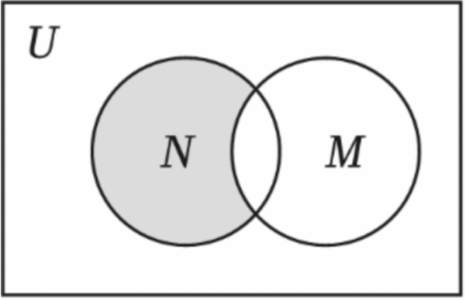
\includegraphics[width=0.30\textwidth]{figures/gao90_q6_venn.png}
\end{center}

\ifanswer
\ans{$N\cap\overline M$}
\fi

\item 已知 $a\in\R$，若关于 $x$ 的方程 $x^2-2x+a-2=0$ 有两个实根 $x_1$、$x_2$，且 $\dfrac1{x_1}+\dfrac1{x_2}=-\dfrac12$，则 $a$ 的值为\blankline[4.4em].

\ifanswer
\solbegin
\step{由于 $x_1$、$x_2$ 是 $x^2-2x+a-2=0$ 的两个实根，}
\step{由韦达定理得 $x_1x_2=a-2$，$x_1+x_2=2$，}
\step{因此 $\dfrac1{x_1}+\dfrac1{x_2}=\dfrac{x_1+x_2}{x_1x_2}=\dfrac2{a-2}=-\dfrac12$，所以 $a-2=-4$，解得 $a=-2$，}
\step{判别式 $\Delta=(-2)^2-4(a-2)=-4a+12$，当 $a=-2$ 时，$\Delta=8+12=20>0$，有两个实根，符合条件，故 $a=-2$.}
\solend
\fi

\item 如果 $-1<x<4$，$-6<y<2$，则 $2x-y$ 的取值范围是\blankline[4.4em].

\ifanswer
\solbegin
\step{因为 $-1<x<4$，$-6<y<2$，所以 $-2<2x<8$，$-2<-y<6$，}
\step{则 $-2+(-2)<2x-y<8+6$，即 $-4<2x-y<14$，}
\step{故 $2x-y$ 的取值范围为 $(-4,14)$.}
\solend
\fi

\item 集合 $A=\left\{x\left|\dfrac6{3-x}\in\Z,x\in\N\right.\right\}$，试用列举法表示集合 $A=\blankline[4.4em]$.

\ifanswer
\solbegin
\step{集合 $A=\left\{x\left|\dfrac6{3-x}\in\Z,x\in\N\right.\right\}$，所以 $3-x$ 可取的值有 $\pm1$、$\pm2$、$\pm3$、$\pm6$，}
\step{又因为 $x\in\N$，所以 $x\in\{0,1,2,4,5,6,9\}$，即 $A=\{0,1,2,4,5,6,9\}$.}
\solend
\fi

\item 不等式 $x^2-ax-b<0$ 的解集是 $(2,3)$，若关于 $x$ 的不等式组 $\begin{cases}(x-a)(3x+b)<0\\ x>t\end{cases}$ 没有实数解，则实数 $t$ 的取值范围是\blankline[4.4em].

\ifanswer
\solbegin
\step{因为等式 $x^2-ax-b<0$ 的解集是 $(2,3)$，所以 $x^2-ax-b=0$ 的根为 $2$、$3$，}
\step{所以 $2+3=a$，$2\times3=-b$，所以 $a=5$，$b=-6$，}
\step{由 $(x-a)(3x+b)=(x-5)(3x-6)<0$ 得 $2<x<5$，}
\step{若关于 $x$ 的不等式组 $\begin{cases}(x-a)(3x+b)<0\\ x>t\end{cases}$ 没有实数解，则 $t\geqslant5$.}
\solend
\fi

\item 若方程 $x^2+2x-m=0$ 有解，则 $m\geqslant a$ 为真命题，则 $a$ 的取值范围为\blankline[4.4em].

\ifanswer
\solbegin
\step{因为方程 $x^2+2x-m=0$ 有解，}
\step{所以 $\Delta=2^2-4\times1\times(-m)=4+4m\geqslant0$，解得 $m\geqslant-1$，}
\step{命题“若方程有解，则 $m\geqslant a$”为真命题，即 $\forall m\in[-1,+\infty)$，$m\geqslant a$ 恒成立，}
\step{因此 $a$ 的取值不能超过集合 $[-1,+\infty)$ 的最小值，即 $a\leqslant-1$，}
\step{综上，$a$ 的取值范围为 $(-\infty,-1]$.}
\solend
\fi

\item 设数集 $M=\left\{x\left|m\leqslant x\leqslant m+\dfrac45\right.\right\}$，$N=\left\{x\left|n-\dfrac14\leqslant x\leqslant n\right.\right\}$，且集合 $M$、$N$ 都是集合 $U=\{x\mid0\leqslant x\leqslant1\}$ 的子集，如果把 $b-a$ 称为非空集合 $\{x\mid a\leqslant x\leqslant b\}$ 的“长度”，那么集合 $M\cap N$ 的“长度”的取值范围为\blankline[4.4em].

\ifanswer
\solbegin
\step{注意到集合 $M$ 的长度为 $\dfrac45$，集合 $N$ 的长度为 $\dfrac14$，均为定值，}
\step{要使得 $M\cap N$ 的“长度”最小，则 $M$ 和 $N$ 尽可能分散到区间的两边，}
\step{长度最小为 $\dfrac45+\dfrac14-1=\dfrac1{20}$；}
\step{要使得 $M\cap N$ 的“长度”最大，则 $M$ 和 $N$ 尽可能集中，}
\step{长度最大就是集合 $N$ 的长度，为 $\dfrac14$，}
\step{故集合 $M\cap N$ 的“长度”的取值范围为 $\left[\dfrac1{20},\dfrac14\right]$.}
\solend
\fi

\end{enumerate}

\bigsec{二、选择题}

\begin{enumerate}
\setcounter{enumi}{12}

\item 设集合 $A=\{x\mid x=2k+1,k\in\Z\}$，$B=\{x\mid x=2k-1,k\in\Z\}$，则 $A$、$B$ 之间的关系是\mbox{（\quad）}

\keepwithprev
A. $B\subsetneq A$\qquad B. $A\subsetneq B$\qquad C. $A=B$\qquad D. 以上都不是

\ifanswer
\solbegin
\step{因为 $k\in\Z$，所以 $2k+1$ 与 $2k-1$ 均表示全体奇数，}
\step{即集合 $A=\{x\mid x=2k+1,k\in\Z\}$ 与 $B=\{x\mid x=2k-1,k\in\Z\}$}
\step{都表示全体奇数构成的集合，所以 $A=B$. 故选 $C$.}
\solend
\fi

\item 已知 $a$、$b\in\R$，且 $a>b$，则下列不等式中一定成立的是\mbox{（\quad）}

\keepwithprev
A. $a+1>b$\qquad B. $a>b+1$\qquad C. $a+1<b+1$\qquad D. $a-1<b-1$

\ifanswer
\solbegin
\step{因为 $a>b$，所以 $a+1>b+1$，$a-1>b-1$，故 $CD$ 错误；}
\step{因为 $a>b$，所以 $a+1>b+0$，即 $a+1>b$ 恒成立，故 $A$ 正确；}
\step{取 $a=1$，$b=0$，$B$ 显然错误.}
\step{故选 $A$.}
\solend
\fi

\item 设 $a$、$b\in\R$，“$a+b>2$ 且 $ab>1$”是“$a>1$，$b>1$”的\mbox{（\quad）}

\keepwithprev
A. 充分不必要条件\qquad B. 必要不充分条件

C. 充要条件\qquad D. 既不充分又不必要条件

\ifanswer
\solbegin
\step{因为 $a>1$ 且 $b>1$，所以 $a+b>2$ 且 $ab>1$，}
\step{若已知 $a+b>2$ 且 $ab>1$，可取 $a=\dfrac12$，$b=8$，也满足已知，}
\step{所以“$a+b>2$ 且 $ab>1$”是“$a>1$ 且 $b>1$”的必要不充分条件，故选 $B$.}
\solend
\fi

\item 设集合 $P_1=\{x\mid x^2+ax+1>0\}$，$P_2=\{x\mid x^2+ax+2>0\}$，$Q_1=\{x\mid x^2+x+b>0\}$，$Q_2=\{x\mid x^2+2x+b>0\}$，其中 $a$、$b\in\R$，下列说法中正确的是\mbox{（\quad）}

\keepwithprev
A. 对任意 $a$，$P_1$ 是 $P_2$ 的子集，对任意 $b$，$Q_1$ 不是 $Q_2$ 的子集

B. 对任意 $a$，$P_1$ 是 $P_2$ 的子集，存在 $b$，使得 $Q_1$ 是 $Q_2$ 的子集

C. 存在 $a$，使得 $P_1$ 不是 $P_2$ 的子集，对任意 $b$，$Q_1$ 不是 $Q_2$ 的子集

D. 存在 $a$，使得 $P_1$ 不是 $P_2$ 的子集，存在 $b$，使得 $Q_1$ 是 $Q_2$ 的子集

\ifanswer
\solbegin
\step{对于集合 $P_1=\{x\mid x^2+ax+1>0\}$，$P_2=\{x\mid x^2+ax+2>0\}$，}
\step{得当 $m\in P_1$ 时，即 $m^2+am+1>0$，得 $m^2+am+2>0$，}
\step{即有 $m\in P_2$，得对任意 $a$，$P_1$ 是 $P_2$ 的子集，}
\step{对于集合 $Q_1=\{x\mid x^2+x+b>0\}$，$Q_2=\{x\mid x^2+2x+b>0\}$，}
\step{当 $b=6$ 时，$Q_1=\{x\mid x^2+x+6>0\}=\R$，$Q_2=\{x\mid x^2+2x+6>0\}=\R$，}
\step{得 $Q_1$ 是 $Q_2$ 的子集，}
\step{当 $b=1$ 时，$Q_1=\{x\mid x^2+x+1>0\}=\R$，}
\step{$Q_2=\{x\mid x^2+2x+1>0\}=\{x\mid x\neq-1\}$，得 $Q_1$ 不是 $Q_2$ 的子集，}
\step{所以存在 $b$，使得 $Q_1$ 是 $Q_2$ 的子集，故选 $B$.}
\solend
\fi

\end{enumerate}

\bigsec{三、解答题}

\begin{enumerate}
\setcounter{enumi}{16}

\item 若 $a$、$b\in\R$，求关于 $x$ 的不等式 $ax\geqslant b$ 的解集.

\ansspace*[9]

\ifanswer
\solbegin
\step{当 $a>0$ 时，原不等式的解集为 $\left\{x\left|x\geqslant\dfrac ba\right.\right\}$；}
\step{当 $a<0$ 时，原不等式的解集为 $\left\{x\left|x\leqslant\dfrac ba\right.\right\}$；}
\step{当 $a=0$，$b\leqslant0$ 时，原不等式的解集为 $\R$；}
\step{当 $a=0$，$b>0$ 时，原不等式的解集为 $\varnothing$.}
\solend
\fi

\item 设集合 $A=\{x\mid x^2+3x+2=0\}$，$B=\{x\mid x^2+(m+1)x+m=0\}$.

（1）用列举法表示集合 $A$；

（2）若 $B\subseteq A$，求实数 $m$ 的值.

\ansspace*[9]

\ifanswer
\solbegin
\stepm{（1）}{集合 $A=\{x\mid x^2+3x+2=0\}$，解方程 $x^2+3x+2=0$，得 $x_1=-2$，$x_2=-1$，}
\step{所以 $A=\{-2,-1\}$.}
\stepm{（2）}{$A=\{-2,-1\}$，$B=\{x\mid x^2+(m+1)x+m=0\}=\{x\mid(x+1)(x+m)=0\}$，}
\step{$B\subseteq A$，所以 $m=1$ 或 $m=2$，所以实数 $m$ 的值为 $1$ 或 $2$.}
\solend
\fi

\item （1）设 $a$、$b$ 是两个正数. 已知 $a>b$，比较 $\dfrac{2a+b}{a+2b}$ 与 $\dfrac ab$ 的值的大小.

（2）用反证法证明：若 $a$、$b\in\R$，且 $x=a^2-2b+1$，$y=b^2-2a+1$，则 $x$、$y$ 中至少有一个不小于 $0$.

\ansspace*[12]

\ifanswer
\solbegin
\stepm{（1）}{$\dfrac{2a+b}{a+2b}-\dfrac ab=\dfrac{b(2a+b)}{b(a+2b)}-\dfrac{a(a+2b)}{b(a+2b)}=\dfrac{b(2a+b)-a(a+2b)}{b(a+2b)}$}
\step{$=\dfrac{2ab+b^2-a^2-2ab}{b(a+2b)}=\dfrac{b^2-a^2}{b(a+2b)}=\dfrac{(b+a)(b-a)}{b(a+2b)}$，}
\step{又 $a>0$，$b>0$，$a>b$，所以 $b+a>0$，$b-a<0$，$b(a+2b)>0$，}
\step{所以 $\dfrac{(b+a)(b-a)}{b(a+2b)}<0$，即 $\dfrac{2a+b}{a+2b}-\dfrac ab<0$，所以 $\dfrac{2a+b}{a+2b}<\dfrac ab$.}
\stepm{（2）}{假设 $x$、$y$ 都小于 $0$，则有 $x+y<0$，}
\step{因为 $x=a^2-2b+1$，$y=b^2-2a+1$，}
\step{所以 $x+y=(a^2-2b+1)+(b^2-2a+1)=(a^2-2a+1)+(b^2-2b+1)$}
\step{$=(a-1)^2+(b-1)^2$，}
\step{又 $a$、$b\in\R$，所以 $(a-1)^2\geqslant0$，$(b-1)^2\geqslant0$，即 $x+y\geqslant0$，}
\step{这与 $x+y<0$ 矛盾，故假设不成立，所以 $x$、$y$ 中至少有一个不小于 $0$.}
\solend
\fi

\item 已知 $m>0$，$p:(x+1)(x-5)\leqslant0$，$q:1-m\leqslant x\leqslant1+m$.

（1）若 $m=5$，$p$、$q$ 有且只有一个为真命题，求实数 $x$ 的取值范围；

（2）若 $p$ 是 $q$ 的充分不必要条件，求实数 $m$ 的取值范围.

\ansspace*[12]

\ifanswer
\solbegin
\stepm{（1）}{对于 $p:(x+1)(x-5)\leqslant0$，解得 $-1\leqslant x\leqslant5$，}
\step{若 $m=5$，则 $q:-4\leqslant x\leqslant6$，}
\step{若 $m=5$，$p$、$q$ 有且只有一个为真命题，则 $p$ 真 $q$ 假或 $p$ 假 $q$ 真，}
\step{若 $p$ 真 $q$ 假，即 $\begin{cases}-1\leqslant x\leqslant5\\ x<-4\ \text{或}\ x>6\end{cases}$，无解，}
\step{若 $p$ 假 $q$ 真，即 $\begin{cases}x<-1\ \text{或}\ x>5\\ -4\leqslant x\leqslant6\end{cases}$，解得 $-4\leqslant x<-1$ 或 $5<x\leqslant6$，}
\step{综上，$-4\leqslant x<-1$ 或 $5<x\leqslant6$，即 $x$ 的取值范围为 $[-4,-1)\cup(5,6]$；}
\stepm{（2）}{若 $p$ 是 $q$ 的充分条件，则有 $\begin{cases}1-m\leqslant-1\\ 5\leqslant1+m\end{cases}$，解得 $m\geqslant4$，}
\step{即 $m$ 的取值范围为 $[4,+\infty)$.}
\solend
\fi

\item 已知关于 $x$ 的不等式：$ax^2-(a+1)x+1<0(a\in\R)$.

（1）当 $a=-2$ 时，求不等式的解集；

（2）当 $a\geqslant0$ 时，求不等式的解集；

（3）命题 $P$：若二次不等式 $ax^2-(a+1)x+1<0$ 的解集为空集，命题 $Q:x^2-2x-a^2+a+1>0$ 对任意实数 $x$ 都成立，若 $P$、$Q$ 中至少有一个真命题，求实数 $a$ 的取值范围.

\ansspace*[14]

\ifanswer
\solbegin
\stepm{（1）}{当 $a=-2$ 时，原不等式为 $2x^2-x-1>0$，即 $(x-1)(2x+1)>0$，}
\step{解得 $x<-\dfrac12$ 或 $x>1$，所以原不等式的解集为 $\left(-\infty,-\dfrac12\right)\cup(1,+\infty)$.}
\stepm{（2）}{当 $a=0$ 时，原不等式为 $-x+1<0$，解得 $x>1$；}
\step{当 $a>0$ 时，原不等式变为 $(ax-1)(x-1)<0$，其对应方程的两根为 $\dfrac1a$，$1$，}
\step{若 $\dfrac1a<1$，即 $a>1$ 时，由 $(ax-1)(x-1)<0$ 解得 $\dfrac1a<x<1$，}
\step{若 $\dfrac1a=1$，即 $a=1$ 时，不等式 $(ax-1)(x-1)<0$ 解集为 $\varnothing$，}
\step{若 $\dfrac1a>1$，即 $0<a<1$ 时，由 $(ax-1)(x-1)<0$ 解得 $1<x<\dfrac1a$，}
\step{综上，当 $a=0$ 时，不等式的解集为 $(1,+\infty)$，}
\step{当 $0<a<1$ 时，不等式的解集为 $\left(1,\dfrac1a\right)$，}
\step{当 $a=1$ 时，不等式的解集为 $\varnothing$，}
\step{当 $a>1$ 时，不等式的解集为 $\left(\dfrac1a,1\right)$.}
\stepm{（3）}{若命题 $P$ 为真命题，}
\step{若 $a<0$，原不等式变为 $(ax-1)(x-1)<0$，其对应方程的两根为 $\dfrac1a$，$1$，}
\step{其解集为 $\left(-\infty,\dfrac1a\right)\cup(1,+\infty)$，不合题意，}
\step{当 $a\geqslant0$ 时，由（2）得当 $a=1$ 时，解集为 $\varnothing$，}
\step{所以命题 $P$ 为真命题，则 $a=1$；}
\step{命题 $Q$ 为真命题，则有相应方程的 $\Delta<0$，即 $a^2-a<0$，解得 $0<a<1$；}
\step{所以当命题 $P$、$Q$ 都为假命题时，$\begin{cases}a\leqslant0\ \text{或}\ a\geqslant1\\ a\neq1\end{cases}$，解得 $a\leqslant0$ 或 $a>1$，}
\step{所以命题 $P$、$Q$ 中至少有一个真命题，则 $0<a\leqslant1$.}
\step{所以实数 $a$ 的取值范围为 $(0,1]$.}
\solend
\fi

\end{enumerate}

\end{document}
